\documentclass{article}
\usepackage{amsmath}
\usepackage{amssymb}
\usepackage{amsfonts}
\usepackage{epsfig}
\usepackage{theorem}
\usepackage{longtable}

\usepackage{url}
\usepackage{moreverb}
\usepackage{fancyhdr}
\usepackage{geometry}
\usepackage{times}
\usepackage{titlesec}
\usepackage{ragged2e}
\usepackage{graphicx}
\usepackage{xcolor}
\usepackage{comment}

% % % % % % % % % % % % % % % % % % % % % % % % % % % % % % % % % % % % 
\usepackage[normalem]{ulem} % For \sout
\usepackage[ruled]{algorithm2e}

% % % % % % % % % % % % % % % % % % % % % % % % % % % % % % % % % % % %

\usepackage{hyperref}
\usepackage{xspace}
\usepackage{cite}
\usepackage{framed}
\usepackage{algpseudocode} 
\usepackage{longtable}
\usepackage[capitalise,nameinlink,noabbrev]{cleveref}
\usepackage{url}
\usepackage{etoolbox}
\usepackage{fullwidth}

\newbool{showcomments}
\booltrue{showcomments}% comment this to hide comments




%============================



\DeclareMathOperator*{\argmin}{arg\,min}
\DeclareMathOperator*{\argmax}{arg\,max}

\DeclareMathOperator*{\arginf}{arg\,inf}
\DeclareMathOperator*{\argsup}{arg\,sup}

% \newcommand{\symboldefinition}[4]{#1}


\newcommand{\ehuffo}{{\epsilon_{\textrm{huff, 1}}}}
\newcommand{\ehufft}{{\epsilon_{\textrm{huff, 2}}}}
\newcommand{\mhufft}{{M_{\textrm{huff, 2}}}}



\newcommand{\activeconstraintsk}{{\mathbb A_{k}}}
\newcommand{\activeconstraintsl}{{\mathbb A_{l}}}
\newcommand{\activeconstraintskpo}{{\mathbb A_{k+1}}}

\newcommand{\atr}{A^{\infty}}
\newcommand{\btr}{b^{\infty}}

\newcommand{\bpr}{{B_{\infty}\left(p, r\right)}}
\newcommand{\bs}{{\beta^{(\star, k)}}}
\newcommand{\bsk}{{\beta_0^{(\star, k)}}}
\newcommand{\capcones}{{C^{(k)}_{\cap}}}
\newcommand{\capconeskmo}{{C^{(k-1)}_{\cap}}}
\newcommand{\chik}{{\chi_m^{(k)}}}
\newcommand{\chil}{{\chi_m^{(l)}}}
\newcommand{\ck}{c^{(k)}}
\newcommand{\ckpo}{{c^{(k+1)}}}
\newcommand{\dacc}{{\Delta_{\textrm{acc}}}}
\newcommand{\dacco}{{\Delta_{\textrm{a}}}}
\newcommand{\deltalargzik}{{\Delta_{\alpha,\beta}}}
\newcommand{\dfeas}{{\Delta_{\textrm{feasible}}}}
\newcommand{\dk}{\Delta_k}
\newcommand{\dl}{\Delta_l}
\newcommand{\dkpo}{\Delta_{k+1}}
\newcommand{\dsr}{{\Delta_{\textrm{sr}}}}
\newcommand{\fcki}{{C^{(k+1)}_{\textrm{in}}}}
\newcommand{\feasiblek}{{\mathcal F_m^{(k)}}}
\newcommand{\feasiblekmo}{{\mathcal F_m^{(k-1)}}}
\newcommand{\feasiblel}{{\mathcal F_m^{(l)}}}
\newcommand{\feasible}{{\mathcal F}}
\newcommand{\fmin}{f_{\text{min}}}
\newcommand{\gammabi}{\gamma_{\textrm{suff}}}
\newcommand{\gammasm}{\gamma_{\textrm{min}}}
\newcommand{\gcik}{{\nabla c_i \left(\xk\right)}}
\newcommand{\gk}{{\nabla m_f^{(k)}\left(\xk\right)}}
\newcommand{\gl}{{\nabla m_f^{(l)}\left(\xl\right)}}
\newcommand{\gmcik}{{\nabla m_{c_i}^{(k)}\left(\xk\right)}}
\newcommand{\gmcikmo}{{\nabla m_{c_i}^{(k-1)}\left(\xk\right)}}  
\newcommand{\gmcil}{{\nabla m_{c_i}^{(l)}\left(\xl\right)}}
\newcommand{\gradf}{\nabla f}
\newcommand{\hgik}{{\frac{\nabla m^{(k)}_{c_i}(\xk)}{\|\nabla m^{(k)}_{c_i}\left(\xk\right)\|}}}
\newcommand{\hk}{{\nabla^2m_f^{(k)}\left(\xk\right)}}
\newcommand{\huff}{{\Gamma_0}}
\newcommand{\huk}{{{\hat u}^{(k)}}}
\newcommand{\lipgrad}{{L_{\nabla}}}
\newcommand{\liphess}{{L_{\nabla^2}}}
\newcommand{\maxgrad}{{M_{\nabla}}}
\newcommand{\maxhessian}{{M_{\nabla^2}}}
\newcommand{\maxmodelhessian}{{M_{\nabla^2 m}}}
\newcommand{\maxnorm}{{M_{\|\cdot\|}}}
\newcommand{\mcik}{{{m}^{(k)}_{c_i}}}
\newcommand{\mcikmo}{{{m}^{(k-1)}_{c_i}}}
\newcommand{\mcil}{{{m}^{(l)}_{c_i}}}
\newcommand{\mck}{{{m}_{c}}^{(k)}}
\newcommand{\mf}{{{m}_f}}
\newcommand{\mfk}{{{m}_f}^{(k)}}
\newcommand{\mfkmo}{{{m}_f}^{(k-1)}}
\newcommand{\minactivegraddelta}{{\Delta_{\mathcal A}}}
\newcommand{\minactivegrad}{{ g_{\mathcal A} }}
\newcommand{\minanglealpha}{{ \alpha^{\star} }}
\newcommand{\minangledelta}{{\Delta_{\alpha^{\star}}}}
\newcommand{\mingraddelta}{{\Delta_{\nabla c}}}
\newcommand{\mingradepsilon}{{\epsilon_{\nabla c}}}
\newcommand{\mingrad}{{ g_{\textrm{low}} }}
\newcommand{\naturals}{\mathbb N}
\newcommand{\oalpha}{\tau_{\Delta}}
\newcommand{\omegadec}{\omega_{\text{dec}}}
\newcommand{\omegainc}{\omega_{\text{inc}}}
\newcommand{\outertrk}{{T_{\text{out}}^{(k)}}}
\newcommand{\outertrkpo}{{T_{\text{out}}^{(k+1)}}}
\newcommand{\polydn}{\mathcal{P}^d_n}
\newcommand{\qk}{{Q^{(k)}}}
\newcommand{\reals}{\mathbb R}
\newcommand{\rk}{\rho_k}
\newcommand{\Rm}{\mathbb R^m}
\newcommand{\Rn}{\mathbb R^n}
\newcommand{\rotk}{{R^{(k+1)}}}
\newcommand{\sampletrk}{{T_{\text{sample}}^{(k)}}}
\newcommand{\sampletrkpo}{{T_{\text{sample}}^{(k+1)}}}
\newcommand{\sampletrkmo}{{T_{\text{sample}}^{(k-1)}}}
\newcommand{\scaledunshiftedellipsoid}{{{\mathcal {\hat E}_{\text{feasible}}}^k}}
\newcommand{\sdk}{\delta_k}
\newcommand{\searchtrk}{{T_{\text{search}}^{(k)}}}
\newcommand{\sigmamax}{{\sigma_{\textrm{max}}}}
\newcommand{\sk}{{{s}^{(k)}}}
\newcommand{\thetamink}{{\pi^k_{\textrm{min}}}}
\newcommand{\tolcrit}{\tau_{\xi}}
\newcommand{\tolrad}{\tau_{\Delta}}
\newcommand{\trk}{\outertrk}
\newcommand{\trkpo}{\outertrkpo}
\newcommand{\trsinfset}{{E_\textrm{infeasible}}}
\newcommand{\trstol}{{\delta_\textrm{infeasible}}}
\newcommand{\unshiftedellipsoid}{{\mathcal E^k_{\textrm{feasible}}}}
\newcommand{\wik}{{w^{(i, k)}}}
\newcommand{\ximin}{\xi_{\text{min}}}
\newcommand{\xkpo}{{{x}^{(k+1)}}}
\newcommand{\xk}{x^{(k)}}
\newcommand{\xki}{x_i^{(k)}}
\newcommand{\xl}{{x^{(l)}}}
\newcommand{\xinit}{{x^{(0)}}}
\newcommand{\zik}{{z^{(i, k)}}}
\newcommand{\zil}{{z^{(i, l)}}}
\newcommand{\deltamingrad}{{\Delta_{\textrm{mm}}}}
\newcommand{\mingradmodel}{{ g_{\textrm{mm}} }}
\newcommand{\activefeasiblek}{{\mathcal F^{(k)}_A}}
\newcommand{\activechik}{{\chi_A^{(k)}}}
\newcommand{\qkmo}{{Q^{(k-1)}}}
\newcommand{\qkpo}{{Q^{(k+1)}}}
\newcommand{\ckmo}{{c^{(k-1)}}}
\newcommand{\sdkmo}{\delta_{k-1}}
\newcommand{\sdkpo}{{\delta_{k+1}}}
\newcommand{\projk}{{p^{(k)}}}
\newcommand{\projl}{{p^{(l)}}}
\newcommand{\projkl}{{p^{(k,l)}}}
\newcommand{\projlk}{{p^{(l,k)}}}
\newcommand{\projkk}{{p^{(k,k)}}}
\newcommand{\projll}{{p^{(l,l)}}}
\newcommand{\trueprojk}{{p_c^{(k)}}}
\newcommand{\truefeasiblek}{{F_c^{(k)}}}
\newcommand{\trueactiveprojk}{{\mathbb P_c^{(k)}}}
\newcommand{\nearlyactiveprojk}{{\mathbb P_{a}}}
\newcommand{\activeprojkk}{{\mathbb P^{(k, k)}}}
\newcommand{\activeprojkl}{{\mathbb P^{(k, l)}}}
\newcommand{\activeprojlk}{{\mathbb P^{(l, k)}}}
\newcommand{\activeprojll}{{\mathbb P^{(l, l)}}}
\newcommand{\unshiftedellipsoidpo}{{\mathcal E^{k+1}_{\textrm{feasible}}}}
\newcommand{\scaledunshiftedellipsoidpo}{{{\mathcal {\hat E}_{\text{feasible}}}^{k+1}}}
\newcommand{\unshiftedellipsoidkpo}{{\mathcal E^{k+1}_{\textrm{feasible}}}}
\newcommand{\image}{{\textrm{im}}}
\newcommand{\maxmodelgrad}{{M_{\nabla m}}}
\newcommand{\minangleu}{{replace me}}
\newcommand{\minanglediralt}{{w_f}}
\newcommand{\minangledir}{{u_{f not used anymore}}}
\newcommand{\minangledirk}{{u^{(k)}_f}}
\newcommand{\minangledirx}{{u_{f}(x_0)}}
\newcommand{\minangledirl}{{u^{(l)}_f}}
\newcommand{\epsactive}{{\mathbb A_c}}
\newcommand{\epsactivemodels}{{\mathbb A_{m}}}
\newcommand{\fik}{{C^{(i, k)}}}
\newcommand{\suffiterates}{{\mathcal K_{\textrm{suff}}}}
\newcommand{\miniterates}{{\mathcal K_{\textrm{min}}}}
\newcommand{\reduceiterates}{{\mathcal K_{\textrm{sr}}}}
\newcommand{\theircnot}{{\kappa_1}}
\newcommand{\theirc}{{\kappa_2}}
\newcommand{\zikthresh}{{ K_{\textrm{a}} }}
\newcommand{\jackk}{{J^{(k)}}}
\newcommand{\jackl}{{J^{(l)}}}
\newcommand{\jackkl}{{J^{(k)}_{\activeprojkk \cup \activeprojkl}}}
\newcommand{\jaclkl}{{J^{(l)}_{\activeprojkk \cup \activeprojkl}}}
\newcommand{\jackt}{{J^{(k)}_{\activeprojkk \cup \trueactiveprojk}}}
\newcommand{\huffeps}{{\epsilon_h}}
\newcommand{\huffalpha}{{\alpha_h}}
\newcommand{\huffdir}{{u_h}}
\newcommand{\huffdirk}{{u^{(k)}_h}}
\newcommand{\activeprojk}{{\textrm{active projection k}}}
\newcommand{\activeprojl}{{active projection l}}
\newcommand{\ulb}{{\mathcal U\left(\epsilon_{\textrm{lb}}\right)}}
\newcommand{\elb}{{\epsilon_{\textrm{lb}}}}
\newcommand{\slb}{{S_{\textrm{lb}}\left(\epsilon_{\textrm{lb}}\right)}}
\newcommand{\dlb}{{\Delta_{\textrm{lb}}\left(\epsilon_{\textrm{lb}}\right)}}


\newcommand{\convexdistance}{{D}}





\newcommand{\activeindicesk}{{ \mathbb I_h^{(k)} }}
\newcommand{\huffindicesk}{{ \mathbb H_h^{(k)} }}
\newcommand{\inactiveindicesk}{{ \mathbb J_h^{(k)} }}
\newcommand{\huffthreshold}{{\Delta_{\textrm{H}}}}


\newcommand{\deltalb}{{\delta_{\textrm{min}}}}


\newcommand{\minactivealpha}{{ \alpha_{\textrm{h}} }}
\newcommand{\activedirk}{{ u_{h}^{(k)} }}
\newcommand{\activegradmin}{{ g_{\textrm{h}} }}


\newcommand{\modeljack}{{ \nabla m^{(k)}_{c}\left(\xk\right) }}
\newcommand{\modeljacl}{{ \nabla m^{(l)}_{c}\left(\xl\right) }}
\newcommand{\truejack}{{ \nabla c\left(\xk\right) }}


\newcommand{\zmk}{{z_m^{(k, k)}}}
\newcommand{\zlk}{{z_l^{(k, l)}}}
\newcommand{\zck}{{z_c^{(k)}}}

\newcommand{\Amk}{{\mathbb A_m^{(k, k)}}}
\newcommand{\Alk}{{\mathbb A_l^{(k, l)}}}
\newcommand{\Ack}{{\mathbb A_c^{(k)}}}



% Added by Steve
\newcommand{\st}{\textrm{such that}}
\newcommand{\norm}[1]{{\left\|#1\right\|}}
\newcommand{\intr}{\operatorname{int}}





% Need to remove
\newcommand{\domain}{\Omega}
\newcommand{\dmax}{{\Delta_{\textrm{max}}}}
\newcommand{\ellipsek}{{E^{(k)}}}
\newcommand{\scaledellipsek}{{{\hat E}^{(k)}}}
\newcommand{\ak}{{\nabla m_c^{(k)}\left(\xk\right)}}
\newcommand{\bk}{{m_c^{(k)}\left(\xk\right)}}

\newcommand{\lca}{{A}}
\newcommand{\lcb}{{b}}
\newcommand{\lctra}{G^{(k)}}
\newcommand{\lctrb}{{g^{(k)}}}


\newcommand{\uk}{{\huk}}

\newcommand{\activei}{{\mathcal A}}
\newcommand{\alphaone}{{u_{\textrm{feasible}}}}
\newcommand{\alphatwo}{{\pi_1}}
\newcommand{\alphathree}{\pi_2}
\newcommand{\alphak}{\pi^{(k)}}
\newcommand{\alphakp}{\pi_3^{(k)}}
\newcommand{\unshiftedcone}{{C^{(k)}_{\textrm{unsh}}}}
\newcommand{\shiftedcone}{{C^{(k)}_{\textrm{sh}}}}
\newcommand{\deltaf}{\delta_{f}}


\newcommand{\condition}{{\kappa}}
\newcommand{\polyk}{{{\mathcal{P}}^{(k)}}}
\newcommand{\tolsr}{{\tau_{\textrm{ef}}}}
\newcommand{\slin}{{{\hat s}^{(k)}}}

\newcommand{\proj}{{\textrm{Proj}}}



\newcommand{\hullpoly}{\mathcal P_{\textrm{hull}}}
\newcommand{\dgood}{\Delta_{\textrm{fsr}}}



\newcommand{\nocontentsline}[3]{}
\newcommand{\tocless}[2]{\bgroup\let\addcontentsline=\nocontentsline#1{#2}\egroup}



%
% File thesis_environment.tex
%
% Description:
% This file contains environments for theorems, lemmas, definitions,
% proofs, corollaries, algorithms, examples, remarks, and assumptions.
% The numbering is set up so that the same counter is used for ALL
% these environments.  This seems to make it easier for readers to
% find referenced material.  The counter is reset for each chapter.
%
% EXAMPLE
%    Definition 3.1
%    Lemma 3.2
%    Example 3.3
%    Theorem 3.4
%    Theorem 3.5
%    Lemma 3.6 ....
%
%    Lemma 4.1
%    Corollary 4.2 ....
%
% The Definition environment is indented on both sides.  This
% is not required, but seemed to be a nice way to separate definitions
% from proven results.
%
%%%%%%%%%%%%%%%%%%%%%%%%%%%%%%%%%%%%



%============================

\newtheorem{theorem}{Theorem}[chapter]
\newtheorem{corollary}[theorem]{Corollary}
\newtheorem{definition}[theorem]{Definition}
\newtheorem{lemma}[theorem]{Lemma}

% \numberwithin{thoerem}{chapter}



\crefname{equation}{}{equations}

\newcounter{assumptioncounter}
\newenvironment{assumption}[1][]{\refstepcounter{assumptioncounter}\par\medskip
\textbf{Assumption \theassumptioncounter} \rmfamily \itshape}{\medskip}

\numberwithin{assumptioncounter}{chapter}
\crefname{assumptioncounter}{Assumption}{assumption}


\newenvironment{comment}
	{
		\ifbool{showcomments}{
			\par\medskip
			\color{red}%
			\begin{framed}
			\textbf{Comment: }
			\ignorespaces
		}{}
	}
	{
		\ifbool{showcomments}{
			\end{framed}
			\medskip
		}{}
	}


\def\proof{\par{\it Proof}. \ignorespaces}

\def\endproof{\vbox{\hrule height0.6pt\hbox{%
   \vrule height1.3ex width0.6pt\hskip0.8ex
   \vrule width0.6pt}\hrule height0.6pt
  }}

  
  
% \newcommand{\new}[1]{{\color{blue}#1}}
% \newcommand\hcancel[2][black]{\setbox0=\hbox{$#2$}\rlap{\raisebox{.45\ht0}{\textcolor{#1} {\rule{\wd0}{1pt}}}}#2} 
% \newcommand{\replace}[2]{{\color{red}\sout{#1}\color{black}{\color{red}#2\color{black}}}} %TeX source markup.
% \newcommand{\replaceb}[2]{{\color{blue}\sout{#1}\color{black}{\color{blue}#2\color{black}}}} %TeX source markup.
% \newcommand{\replacemath}[2]{{\hcancel[red]{#1}{}{\color{red}#2\color{black}}}} %TeX source markup.
% % \newcommand{\replacemath}[2]{{\color{red}#2\color{black}}} %TeX source markup.
% \newcommand{\replacemathb}[2]{{\hcancel[blue]{#1}{}{\color{blue}#2\color{black}}}} %TeX source markup.

\newcommand{\sbnote}[1]{
	\ifbool{showcomments}{
		\textsf{
			{
				\color{cyan}{ SCB note:}   #1
			}
		}
% 		\marginpar{
% 			{
% 				\textbf{Comment}
% 			}
% 		}
	}{}
}

% \newcommand{\sbnote}[1]{
% 		\textsf{
% 			{
% 				\color{cyan}{ SCB note:}   #1
% 			}
% 		}
% 		\marginpar{
% 			{
% 				\textbf{Comment}
% 			}
% 		}
% }

\newcommand{\outerfritr}{D_{\text{out}}}



\newcommand{\real}{\mathbb R}

\newcommand{\trialk}{{{s}^{(k)}}}
\newcommand{\matvec}{\mathrm{vec}}

\crefname{Lemma}{Lemma}{Lemma}
\crefname{Corollary}{Corollary}{Corollary}

%=========================================

\title{Model-Based Trust Region Methods for Derivative-Free Optimization with Unrelaxable Linear Constraints}
\author{Stephen C.  Billups and Trever Hallock}

\makeatletter
\def\BState{\State\hskip-\ALG@thistlm}
\makeatother

\let\oldref\ref
\renewcommand{\ref}[1]{(\oldref{#1})}
\def\INCLUDEOMITTED{0}
\begin{document}


\maketitle

\begin{abstract}
We propose a model-based trust-region algorithm for constrained optimization problems with linear constraints in which derivatives of the objective function are not available and the objective function values outside the feasible region are not available.
In each iteration, the objective function is approximated by an interpolation model, which is then minimized over a trust region.
To ensure feasibility of all sample points and iterates, we consider two trust region strategies in which the trust regions are contained in the feasible region.
Computational results are presented on a suite of test problems.

\end{abstract}

\newpage

\tableofcontents

\newpage
\section{TO DO}
\begin{enumerate}
\item Shorten literature review
% \item Consider removing material on finding the maximum volume ellipsoid
% \item Remove ellipsoid searches.  Instead, just use the one center defined in the analysis.
% \item Remove polyhedral trust region method.
\end{enumerate}
\section{Introduction}
Derivative-free optimization (DFO) refers to mathematical programs involving functions for which derivative information is not explicitly available.
Such problems arise, for example, when the functions are evaluated by simulations or by laboratory experiments.
Applications of DFO appear in many fields, including photo-injector optimization \cite{Neveu2017},
circuitry arrangements \cite{PLOSKAS201816}, machine learning \cite{KS2018}, volume optimization \cite{Cheng2017}, and reliability-based optimization \cite{Gao2017}.
In such applications, function evaluations are typically expensive, 
so it is sensible to invest significant computational resources to minimize the number of function evaluations required.

This work is aimed at developing algorithms to solve constrained optimization problems of the form 
\begin{align}
\begin{array}{ccl} \min_{x \in \Rn} & f(x) \\
\mbox{subject to} \quad & c_i(x) \le 0, &\quad \forall 1 \le i \le m,
\end{array}
\label{the_dfo_problem}
\end{align}
where 
% $\domain$ is a subset of $\Rn$, and
$f$ and $c_i$ for $1 \le i \le m$ are real-valued functions on $\Rn$ with at least one of these functions being a {\em black-box} function, meaning that derivatives cannot be evaluated directly.
We let the feasible set be represented as
\begin{align}
\feasible = \{x \in \Rn \; | \; c_i(x) \le 0, \; \forall 1 \le i \le m \}.
\end{align}

We are interested in developing {\em model-based}, {\em trust-region} algorithms for solving these problems.
Model-based methods work by constructing model functions to approximate the black box functions at each iteration.
The model functions are determined by fitting previously evaluated function values on a set of sample points.
In trust-region methods, the model functions are used to define a trust-region subproblem whose solution determines the next iterate.
For example, the trust-region subproblem might have the form
\begin{align*}
\begin{array}{ccl} \min_{\|s\| \le \dk}
 & \mfk \left(\xk+s\right) \\
\mbox{subject to} \quad & \mcik\left(\xk + s\right) \le 0 & \quad 1 \le i \le m, \\
& \|s\| \le \dk \\
\end{array}
\end{align*}
where $\xk$ is the current iterate, $\mfk$ is the model function approximating $f$, 
and $\mcik$ are the model functions approximating the constraint functions $c_i, \forall 1 \le i \le m$, and $\dk$ is the radius of the trust-region.
The key differences between the trust-region subproblem problem and the original are that all functions are replaced with their model functions, 
and a trust region constraint ($\|s\| \le \dk$) has been added.

%Note that we are using models of the constraint functions to approximate the feasible region during each iteration.  In particular, we define the {\em model feasible region} by
%\begin{align}
%\feasiblek = \left\{x \in \Rn \big| \mcik(x) \le 0 \quad \forall 1 \le i \le m \right\}.  \label{define_feasiblek}
%\end{align}



Conceptually, the model functions are ``trusted'' only within a distance $ \dk $ of the current iterate $\xk$; 
so the trust-region subproblem restricts the length of step $s$ to be no larger than $\dk$.
To ensure that the model functions are good approximations of the true functions over the trust region, 
the sample points are typically chosen to lie within the trust-region.

%
% {\em quantifiable} means the functions can be evaluated at any point in $\feasible$
% and that the values returned for the constraint functions provide meaningful information about how close the point is to a constraint boundary.
% This means the constraints
% For example, the authors of  apply derivative-free optimization to rapid-cycling synchrotron lattice design.
% The problem has a non-smooth objective and both linear and simulation based unrelaxable constraints.
% These constraints are unrelaxable, because simulation is not possible with overlapping synchrotron elements.
% In this case,  the constraints are called {\em unrelaxable}.
% \sbnote{Can we find an example of an unrelaxable constraint?}
We are specifically interested in applications where some of the black box functions cannot be evaluated outside the feasible region.  Constraints of this type can arise in several ways, such as when a simulation cannot be carried out on particular inputs.
For example, the authors of \cite{Padidar2021} optimize rapid-cycling synchroton lattice design,
but some overlapping synchrotron elements cannot be simulated.
Following the taxonomy in \cite{ledigabel2015taxonomy},  such constraints are called {\em unrelaxable}.

For problems involving unrelaxable constraints,  we require all iterates and sample points to be feasible.
As a first step toward developing algorithms to solve such problems, this paper considers a simplified problem where all of the constraints are linear and unrelaxable; namely:
\begin{align}
\begin{array}{ccl} \min_{x \in \Rn} & f(x) \\
& \lca x \le \lcb, & 
\end{array}
\label{linear_dfo_problem}
\end{align}
where $\lca$ is an $m \times n$ matrix and $\lcb \in \Rm$.
\color{magenta}
We assume that the rows of $A$ have been normalized so that $\|A_i\| = 1$.
\color{black}


An important consideration in fitting the model functions is the ``geometry'' of the sample set.
This will be discussed in more detail in \cref{geometry}, but the key point is that the relative positions of the sample points within the trust region have a significant effect on the accuracy of the model functions over the trust region.
When the geometry of the sample set is poor, it is sometimes necessary to evaluate the functions at new points within the trust region to improve the geometry of the sample set.
It is well understood how to do this for unconstrained problems, but for constrained problems
our requirement that the sample points must be feasible poses some interesting challenges to maintaining good geometry.   

\sbnote{The following new paragraph discusses geometry}

In unconstrained optimization, it is typical and natural for the sample trust region to be centered at the current iterate.
Thus, much of the standard theory (see for example,
 Chapter 3 of \cite{introduction_book}) of sample set geometry assumes the sample points are chosen within a ball centered at the current iterate.
 However, for constrained problems,  this is no longer a useful assumption.
 In particular, when iterates are close to the boundary of the feasible region, it is advantageous to shift the center of the sample trust region away from the current iterate.
 Because of this, we rework some of the standard results to not require a sample point at the center of the sample trust region.


We propose an algorithm for solving \cref{linear_dfo_problem} whose main idea is to construct a feasible ellipsoid at each iteration that lies within the intersection of the feasible region and the current trust region.   We call this ellipsoid the {\em sample trust region}.
To choose well-poised sample points for this ellipsoidal region,  we adapt a model improvement algorithm presented in \cite{introduction_book} for spherical trust regions and establish error bounds on the accuracy of the model functions over this region.    

Our convergence analysis is based on an algorithmic framework presented \cite{Conejo:2013:GCT:2620806.2621814},  which describes a class of trust-region algorithms for convex constrained minimization without derivatives.   This framework assumes that a model of the objective function can be constructed at each iteration that satisfies certain accuracy assumptions, but it does not specify how to construct such a model function.    Here, we show that the model functions constructed by our algorithm satisfy these assumptions.  Hence,  using the results from \cite{Conejo:2013:GCT:2620806.2621814}, we show that
the criticality measure for the iterates generated by our algorithm converges to zero.  As a consequence, any accumulation point of the iterates satisfies the Karush-Kuhn-Tucker first order optimality conditions.  


\subsection{Notation}
\sbnote{Make sure we actually use all of these conventions in the paper.  That is, delete anything used in the thesis that isn't used in the linear constraint paper}


We use:
\begin{itemize}
\item super scripts for iterations
\item subscripts for indices of vector
\item projection
\item $[m]$
\item matrix set-subset notation
\item ball notation
\item norm, frebenious norm
\item set compliment
\item set addition/subtraction
\item Kronecker delta
\item positive part
\end{itemize}



We use the following notational conventions throughout the paper.
Any variables that depend on the iteration will be super-scripted by $k$.
For example, the $k$-th iterate is given by $\xk$,
and the model of the objective function for iteration $k$ is given by $\mfk$.
Subscripts on vectors are used as an index into the vector, while vectors in a sequence of vectors use superscripts:
that is, $\xki$ is the $i$-th component of the $k$-th vector in the sequence $\{\xk\}_k$.
We use $\proj_X(x) = \argmin_{x' \in X}\left\|x' - x\right\|$ to denote the projection of $x$ onto a convex set $X$.
\color{magenta}
It seems like you didn't like this notation. Should I remove it?
\color{black}
For any $m \in \naturals$, we define $[m] = \left\{i \in \naturals | 1 \le i \le m\right\}$.

\paragraph*{Matrices.}
Matrices are denoted with capital letters.
The $i$-th row of the matrix $A$ is denoted $A_i$.
For any index set $S \subseteq \{i \in \naturals | 1 \le i \le m\}$, the $|S| \times n$ matrix formed by only using
rows of the $m\times n$ matrix $A$ from the set $S$ is $A_S$.
Let the condition number of a matrix $Q$ be denoted $\condition(Q)$.
% , while the $i$-th column is denoted $A_{\bullet i}$.
We use $e_i$ to denote the $i$-th unit vector and $e$ to denote the vector of all ones.
$B_k\left(c; \Delta\right)$ is the ball of radius $\Delta$ in the $k$ norm, centered at point $c$.  That is,
\begin{align}
\label{define_ball}
B_k\left(c; \Delta\right) = \left\{x \in \Rn \bigg | \left\|x - c\right\|_k \le \Delta \right\}.
\end{align}
Note that some of the common norms are:
\begin{align*}
\|x\|_{\infty} = \max_{1\le i\le n}|x_i|, \quad
\|x\|_{2} = \sqrt{\sum_{i=1}^n x_i^2}, \quad \textrm{and} \quad
\|x\|_1 = \sum_{i = 1}^n |x_i|.
\end{align*}
When a norm is presented without a subscript, it is assumed to be the $2$ norm: $\|x\| = \|x\|_2$ for any $x \in \Rn$.
For matrices, we will also use the Frobenius norm $\left\|\cdot\right\|_F$ which is $\left\|A\right\|_F = \sqrt{\sum_i\sum_jA_{i, j}^2}$.
% The norm of matrices
% Also, if $A$ is an $n \times n$ matrix, $\|A\|

\paragraph*{Sets.}
The complement of a set $S$ is denoted as $S^c$.
Define a point $x$ subtracted from a set $S$ as $S - x = \left\{s \in \Rn | s - x \in S\right\}$.
Set addition is $X + Y = \left\{x + y | x \in X, y \in Y\right\}$.

$\delta_{i,j}$ is the Kronecker delta, $\delta_{i, j} = \begin{cases} 1 & \textrm{if} \; i = j \\ 0 & \textrm{if} \; i \ne j \end{cases}$.
We define the positive part of a real number to be
\begin{align*}
a^+ = \begin{cases} a & \textrm{if} \quad a \ge 0 \\ 0 & \textrm{otherwise} \end{cases}.\\
\end{align*}

% For any matrix $A$, we let $A^{\dagger}$ be the Moore-Penrose inverse.


\section{Background}
\sbnote{I commented out the literature review for now.  We may not need to have a literature review section.}

%\subsection{Literature Review}
%
%\label{literature_review}
%
%
%% Recently, there has been a growth in applications of derivative-free optimization.
%% Such applications include
%
%% Model based, trust region, I think no constraints, maybe multi-objective:
%% photo-injector optimization \cite{Neveu2017}.
%
%% Direct search, binary constraints, mixed integer (nomad, midaco, glcSolve, CMAES (stochastic))
%% circuitry arrangements \cite{PLOSKAS201816},
%
%% For paralellizable methods, kalman filter methods, optimizing networks
%% machine learning \cite{KS2018}
%
%% Trust region based, reliability surrogate constraints
%% and reliability based optimization \cite{Gao2017}.
%
%% parallel algorim, compares gradient based and dfo, nelder-mead
%% volume optimization \cite{Cheng2017},
%
%Several books and survey articles  provide good introductions to the field of derivative-free optimization.
%Within \cite{introduction_book}, derivative-free methods are developed in detail.
%This is the first textbook devoted to derivative-free optimization.
%It contains an explanation of how to ensure good sample set geometry and introduces the concept of 
%poisedness for unconstrained problems, and it also covers other direct-search and line-search methods.   A review of derivative-free algorithms and software libraries can be found in \cite{miguel_review}.
%This compares several software libraries and reviews the development of derivative-free optimization since it started.
%Other recent reviews can be found in \cite{custodio_review2} and \cite{larson_menickelly_wild_2019}.
%
%Most  algorithms for derivative-free optimization fall into two main categories: direct-search methods and model-based methods.   Direct-search methods use comparatively simple strategies to explore the solution space, using only the relative ranks of function values rather than their numerical values.     Early direct search methods for unconstrained optimization include coordinate descent \cite{fermi.metropolis:numerical},  the Nelder-Mead algorithm \cite{10.1093/comjnl/7.4.308},  
%and pattern search methods \cite {hooke.jeeves:direct, kolda.lewis.ea:optimization}.   Generalizations of pattern-search methods include the GPS method \cite{torczon:convergence, Audet2002AnalysisOG} and the mesh adaptive direct search (MADS) algorithm \cite{audet.dennis:mesh, abramson.audet:convergence}.
%
%Model-based methods guide the search using surrogate models of the black-box functions, which are constructed by fitting function values on a set of sample points.    Among the more commonly used model functions are linear and quadratic interpolation models \cite{ conn.scheinberg.ea:recent, powell:uobyqa,powell:newuoa}  and radial-basis function interpolation models \cite{oeuvray.bierlaire:boosters,wild.regis.ea:orbit,wild.shoemaker:global}.
%
%The use of model functions allows curvature information to be incorporated into the search.  As such, model-based methods tend to be more efficient than direct-search methods when the black box functions are smooth.  In contrast, direct-search methods can be better suited for handling nonsmooth or noisy functions.   They are also more straightforward to implement, and are easier to parallelize.
%
%Hybrid methods, which incorporate ideas from both direct-search and model-based methods, have also been proposed.    Some examples are described in \cite{booker.dennis.ea:rigorous}, \cite{thi.vaz.ea:optimizing}, and \cite{custodio.vicente:using}.
%
%\paragraph*{Constrained derivative-free algorithms.}
%To discuss methods for constrained derivative-free optimization,  we follow the constraint taxonomy      
%of Le~Digabel and Wild \cite{ledigabel2015taxonomy} and distinguish between whether constraints are {\em relaxable} or {\em unrelaxable}.    An unrelaxable constraint is one that {\em must} be satisfied in order to obtain meaningful information about the objective function and/or constraint functions.    Thus algorithms for unrelaxable constraints can use function evaluations only for feasible points.   We also distinguish between whether constraints are {\em algebraic} or {\em black-box}.    A constraint is algebraic if the constraint functions can be computed algebraically,  whereas a {\em black-box constraint} can only be evaluated by running simulation software.    
%
%\paragraph*{Relaxable constraints.}   The easiest class of constraints to deal with are the relaxable algebraic constraints.   In this case, ideas from classical nonlinear programming methods can easily be adapted to the derivative-free setting.  Some examples include 
% penalty methods \cite{lewis.torczon:globally, lewis.torczon:direct, bueno.friedlander.ea:inexact},   and filter methods \cite{brekelmans.driessen.ea:constrained, ferreira.karas.ea:global}.     
%Both penalty methods and filter methods allow iterates to violate constraints, requiring feasibility only in the limit.  As such, they are viable approaches only when the constraints are relaxable.    
% 
%For relaxable black-box constraints,  several methods have been proposed that allow the black-box functions to be evaluated at infeasible points.  These include penalty methods
%\cite{audet.dennis:progressive, liuzzi.lucidi:derivative-free, liuzzi.lucidi.ea:sequential,fasano.liuzzi.ea:linesearch,diniz-ehrhardt.martinez.ea:derivative-free,picheny2016bayesian}, filter methods \cite{audet.dennis:pattern, pourmohamad:combining,echebest.schuverdt.ea:inexact},  and funnel methods \cite{sampaio.toint:derivative-free,sampaio.toint:numerical}.
%
%Another approach is to construct algebraic models of the constraint functions and then require iterates to be feasible with respect to these modelled constraints.
%In \cite{glass.cooper:sequential},  linear models of nearly active constraint functions are constructed and the iterates are accepted only if they are feasible with respect to these modeled constraints.     A similar strategy is employed in the COBYLA method of Powell \cite{powell:direct}, which builds linear models of the objective and constraint functions based on a common set of sample points.    
%A variant of the MADS algorithm is proposed in \cite{burmen.olensek.ea:mesh} which uses linear regression models of the constraint functions to guide the choice of search and poll steps.   In \cite{Troltzsch2016},  the classic sequential quadratic programming algorithm is implemented for equality-based constraints.
%
%
%
%
%%Also, \cite{Gao2018} presents  an algorithm for linearly constrained derivative-free optimization that uses a backtracking technique to minimize the number of evaluations required.
%
%
%
%\paragraph*{Unrelaxable algebraic constraints.}  
%
% An algebraic constraint function can always be evaluated, so the only way it is considered unrelaxable is if a black-box function (either the objective or some other constraint function) cannot be evaluated when the constraint is violated.
%Note that it is always possible to determine whether a point satisfies an algebraic constraint prior to attempting to evaluate any black-box functions.  As such, it is relatively straightforward to modify direct-search methods to guarantee that only feasible points are considered.     
%Many direct-search methods have been proposed that take this approach
%\cite{box:new, spendley.hext.ea:sequential,may:linearly,may:solving,lewis.torczon:globally,lewis.torczon:direct,
%vandenberghen:condor, lewis.torczon:pattern2000,lucidi.sciandrone:derivative-free,chandramouli.narayanan:scaled,kolda.lewis.ea:stationarity,lucidi.sciandrone.ea:objective, 
%audet.ledigabel.ea:linear,gratton.royer.ea:direct2019,gratton.royer.ea:direct2015}
%%
%% \cite{box:new} \cite{spendley.hext.ea:sequential}, \cite{may:linearly}, \cite{may:solving},\cite{lewis.torczon:globally},  \cite{lewis.torczon:direct}, \cite{vandenberghen:condor}, \cite{lewis.torczon:pattern2000} \cite{lucidi.sciandrone:derivative-free}, \cite{chandramouli.narayanan:scaled},  \cite{kolda.lewis.ea:stationarity}, \cite{lucidi.sciandrone.ea:objective}, 
%%\cite{audet.ledigabel.ea:linear},\cite{gratton.royer.ea:direct2019}, \cite{gratton.royer.ea:direct2015}
%  
%Developing model-based algorithms for unrelaxable constraints is complicated by the fact that the choice of sample points impacts the accuracy of the model functions.     Thus, when restrictions on the choice of sample points are imposed,  it can be difficult to ensure that the model functions are sufficiently accurate to guarantee convergence to a stationary point.    (see \cref{sec:polyhedral} for a more detailed explanation of this difficulty).   In the case of unrelaxable bound constraints, the restrictions on the sample points are not too difficult to mitigate.     The BOBYQA algorithm \cite{powell:BOBYQA} ensures that all points at which the objective function are evaluated satisfy the bound constraints, while still maintaining sufficient model accuracy to guarantee convergence.    In \cite{arouxet.echebest.ea:active-set},  an active set method is used when solving the bound-constrained trust-region subproblems.    In \cite{wild:derivative-free}, Wild proposed a radial basis function method for bound constraints, which enforces the bounds when selecting sample points in the model improvement algorithm and when solving the trust region subproblems.   In \cite{gratton.toint.ea:active-set}, Gratton et al. present a method which restricts the construction of the model functions to subspaces defined by nearly active bound constraints.
%
%There has also been some progress in developing model-based methods for unrelaxable linear constraints.   In  \cite{gumma.hashim.ea:derivative-free},  Gumma et al.  propose the LCOBYQA algorithm which is an extension of Powell's NEWUOA algorithm that enforces the linear constraints both when solving the trust region subproblems and when choosing sample points for constructing the model functions.    However, no convergence analysis is provided for the method.   
%
%\paragraph*{Unrelaxable black-box constraints.}   
%We now turn our attention to the hardest case--that of unrelaxable black-box constraints.   In this case,  it is not possible to guarantee that black-box function evaluations will never be attempted at infeasible points.   However, it is desireable to minimize the occurrence of such infeasible attempts.  
%
%There are several strategies for avoiding infeasible evaluations.
%The authors of \cite{Galvan2021} use a reformulation strategy by moving the constraints into the objective.
%Their work relies on a projection operator to avoid infeasible evaluations and handles non-smooth convex constraints.
%The authors of \cite{NOWPAC2014} use a path-augmentation strategy to ensure trial points are feasible.
%This is done with a local convexification of the constraints that parameterize a buffer of the constraints.
%The authors of \cite{BMNORW2020} apply DFO to optimize the Fayans energy density functional, avoiding possible infeasible evaluations by altering the objective function to include a projection onto an $L_1$ ball.
%In \cite{CONORBIT15}, the authors develop a model-based trust region algorithm that uses an envelope to avoid infeasible trial point evaluations.
%The algorithm presented within \cite{Conejo2015} is also a model-based trust region method, and it ensures each iterate is feasible, although sample points may not be.
%More recently, \cite{Brilli2021interior} uses an interior point algorithm to solve derivative-free problems with unrelaxable, black-box constraints.
%
%Of particular importance for our work is \cite{Conejo:2013:GCT:2620806.2621814}.
%This reference provides an elegant convergence proof for a class of algorithms when the constraints are convex.
%Our analysis implements abstractions made in this paper and shows the implementation satisfies their requirements.
%
%%We are not aware of any algorithms that use only feasible points to build models of the black-box constraint functions.   However,  a number of algorithms simultaneously handle unrelaxable algebraic constraints and relaxable black-box constraints.  Thus,  \cite{regis:constrained,augustin.marzouk:nowpac,augustin.marzouk:trust-region,regis.ea:conorbit}.
%
%
%
%%While care is taken to maintain the non-degeneracy of the sample points,  Powell notes that  ``Our %knowledge of the convergence properties for the algorithm is slight.'' 
%
%
%
%
%\pagebreak
%\section{Model-Based Trust-Region Methods for DFO}

The main idea of model-based, trust-region methods is that trial points are selected at each iteration by solving a trust-region subproblem.  
Each subproblem has the form 
\[ \begin{array}{ll} \min_{s \in \Rn} & m_f^{(k)}\left(\xk + s\right) \\ 
\st & \xk+s \in \feasiblek \\
& \norm{s} \le \Delta_k
\end{array} \]
where $m_f^{(k)}$ is a model function approximating the objective $f$, $\dk$ is the trust region radius,
and $\feasiblek$ is an approximation of the feasible region.
The solution $\sk$ of the trust-region subproblem determines a {\em trial point} $\xk + \sk$.  
The objective function and constraints are then evaluated at the trial point to determine whether to accept the trial point.
If the trial point is rejected, the trust region radius is decreased and a new trial point is computed by solving a revised trust-region subproblem.     
If the trial point is accepted, then the trust region radius may be increased or decreased for the next iteration 
depending on how well the sample point improved upon the previous iterate.
This will be discussed in \cref{rhosection}.





\subsection{Interpolation-Based Models}

\label{interpolation}

Model-based methods for derivative-free optimization construct models of a function $f(x)$ from a family of functions spanned by a set of $p + 1 \in \naturals$ basis functions  $\Phi = \{\phi_0, \phi_1, \ldots, \phi_p\}$. Each member of this family has the form $\mf(x) = \sum_{i=0}^p\alpha_i\phi_i(x)$ for some scalar coefficients $\alpha_i, i \in \{0, \ldots, p\}$.

We use interpolation to choose the coefficients $\alpha = [\alpha_0, \ldots, \alpha_p]^T$ so that $\mfk$ agrees with $f$ on a set of $p+1$ sample points $Y = \{y^{(0)}, y^{(1)}, \ldots, y^{(p)}\}$ at which the function $f$ has been evaluated.
Thus, the coefficients $\alpha$ must satisfy the \emph{interpolation condition}
\begin{align}
\label{interpolation_condition}
\mf\left(y^{(i)}\right) = \sum^p_{j=0}\alpha_j\phi_j\left(y^{(i)}\right) = f\left(y^{(i)}\right) \quad \forall \quad 0 \le i \le p.
\end{align}

% We can also write this equation in matrix form.
This equation can be written more compactly in the form
\begin{align}
\label{matrix_form}
M(\Phi,Y) \alpha = \bar{f},
\end{align}
where $\bar{f} = [f\left(y^{(0)}\right), f\left(y^{(1)}\right), \ldots, f\left(y^{(p)}\right)]^T$ and the Vandermonde matrix $M\left(\Phi,Y\right)$ is defined by

\begin{align}
\label{vandermonde}
M\left(\Phi,Y\right) :=
\begin{bmatrix}
    \phi_0\left(y^{(0)}\right)      & \phi_1\left(y^{(0)}\right)       & \ldots & \phi_{p}\left(y^{(0)}\right)      \\
    \phi_0\left(y^{(1)}\right)      & \phi_1\left(y^{(1)}\right)       & \dots  & \phi_{p}\left(y^{(1)}\right)      \\
                     &                   & \vdots &                    \\
    \phi_0\left(y^{(p)}\right)    & \phi_1\left(y^{(p)}\right)     & \ldots & \phi_{p}\left(y^{{(p)}}\right)
\end{bmatrix}.
\end{align}

The interpolation equation \cref{matrix_form} has a unique solution if and only if $M\left(\Phi,Y\right)$ is non-singular.
In this case, we say that the sample set $Y$ is \emph{poised} for interpolation with respect to $\Phi$.   Note also that if $Y$ is poised with respect to one basis for a family of functions, then it is poised with respect to any basis for that family.     
However, even when $M\left(\Phi,Y\right)$ is non-singular,  the interpolation model may be inaccurate if the Vandermonde matrix is poorly conditioned.   Informally,  we say that a sample set is {\em well-poised} if it produces accurate model functions.  The following section formalizes this idea.

\subsection{Sample Set Geometry}

\label{geometry}
The term \emph{geometry} refers to  how the distribution of points in the sample set $Y$ affects the accuracy of the model function.     In the case of polynomial model functions, a rigorous analysis of model accuracy can be performed using \emph{Lagrange polynomials}.
Let the space of polynomials on $\Rn$ with degree less than or equal to $d$ be denoted by $\polydn$ and have dimension $p+1$.
The Lagrange polynomials $\ell_0, \ell_1, \ldots, \ell_p$ for the sample set $Y$ are a basis of $\polydn$ such that
\begin{align}
\ell_i\left(y^{(j)}\right) = \delta_{i,j}  \label{interpolation_condition_lagrange}
\end{align}
where $\delta_{i,j} = \{0 \;\text{if}\; i\ne j,\; 1 \;\text{if} \; i = j \}$ is the Kronecker-delta function.
%For example, after this change of basis, note that the Vandermonde matrix becomes the identity matrix.
Thus, as shown in \cite{introduction_book},  the interpolating model function $\mf(x)$ 
satisfies
\begin{align}
\label{reg} 
\mf(x) = \sum^p_{j=0}f\left(y^{(i)}\right)\ell_i(x).
\end{align}

The following definition allows us to quantify how well-poised a sample set is with respect to interpolation on a polynomial subspace.

\sbnote{Corrected the definition of $\Lambda$-poised.   We don't need a basis for the polynomial space in the definition since the Lagrange polynomials depend only on the space, not the basis.  The definition also needs to include a set $B$}

\color{magenta}
Should $B$ be convex?
\color{black}

\begin{definition}\label{lambda-poised}
\replace{We say that a set $Y$ is \emph{$\Lambda$-poised} for a fixed constant $\Lambda$ with respect to a basis $\Phi$ on the set 
$B \subset\Rn$\\}{Given a fixed constant $\Lambda>0$ and a set $B \subset \Rn$, we say that a sample set $Y$ is \emph{$\Lambda$-poised} in $B$ for interpolation on $\polydn$}
if and only if the Lagrange polynomials $\ell_i$ associated with $Y$ satisfy
\begin{align}
\Lambda \ge \max_{0\le i\le p}\max_{x\in B}|\ell_i(x)|.
\end{align}
\end{definition}

To examine how $\Lambda$-poisedness relates to the accuracy of the interpolation model functions, we shall consider the Vandermonde matrix of a shifted and scaled sample set $\hat{Y} = \frac{1}{\Delta}(Y-\bar{y})$.  The analysis is similar to that presented in \cite{introduction_book}; however their analysis defines a particular  $\hat{Y}$ by choosing $\bar{y} = y^{(0)}$ and $\Delta = \max_{1 \le i \le p} \| y^{(i)}-y^{(0)}\|$.  The resulting set $\hat{Y}$  is contained in the unit ball centered at $\hat{y}^{(0)} = 0$ and has at least one point on the boundary of the ball.    This approach is sensible for unconstrained optimization, where  $y^{(0)}$ is typically chosen to be the current iterate and we are interested in constructing sample sets that are well-poised over the trust region $B_2(y^{(0)};\Delta)$.    However, for constrained optimization,  it is disadvantageous to require the current iterate to be at the center of the sample trust region or to require that there be a sample point on the boundary of the ball.   We therefore consider a more general transformation by specifying an arbitrary center $\bar{y}$ and radius $\Delta$.  

The following result from \cite[Lemmas 3.8 \& 3.9]{introduction_book} shows that the
Lagrange polynomials for a sample set are invariant under a shift or scaling of coordinates.     Hence, the poisedness constant  $\Lambda$ in \cref{lambda-poised}  is also invariant  with respect to a shift or scaling of coordinates. 

\begin{lemma}\label[Lemma]{lagrange_invariance}
Let $Y=\{y^{(0)},\ldots,y^{(p)}\}$ be a set  that is poised for interpolation on $\polydn$.  Let  $\ell_i(x)$,  $i=0,\ldots,p$, be the set of Lagrange polynomials satisfying \cref{interpolation_condition_lagrange} for the set $Y$.   Let $\Delta>0$ and $a \in \Rn$ be given and define the shifted and scaled sample set $\hat{Y}=\left\{\frac{y^{(0)}-a}{\Delta},\dots, \frac{y^{(p)}-a}{\Delta}  \right\}$.
Let $\hat{\ell}_i(x)$, $i=0,\ldots,p$ be the Lagrange polynomials satisfying \cref{interpolation_condition_lagrange} for the set $\hat{Y}$.  Then for any $x \in \Rn$, 
\[ \ell_i(x) = \hat{\ell}_i\left(\frac{x-a}{\Delta}\right),  i=0,\ldots,p.\]
\end{lemma}
 

We now state two technical lemmas that will be used in the proof of our next theorem.

\begin{lemma}(\cite[Lemma 3.10]{introduction_book})
\label[lemma]{lemma_3_10}
Let $\bar \Phi$ be the monomial basis \cref{define_monomial}.
There exists a number $\sigma_{\infty} > 0$ such that, for any choice of $v$ satisfying $\|v\|_{\infty} = 1$,
there exists a $y \in B_2(0; 1)$ such that $\left|v^T\bar \Phi(y)\right| \ge \sigma_{\infty}$.
\end{lemma}

\begin{lemma}(\cite[Lemma 3.13]{introduction_book})
\label[Lemma]{lemma_3_13}
Let $w$ be a normalized right-singular vector of a nonsingular $n \times n$ matrix $A$ corresponding to its largest singular value.
Then, for any vector $r \in \Rn$,
\begin{align*}
\|Ar\| _2\ge |w^T r| \|A\|_2.
\end{align*}
\end{lemma}







The following result, which is a straightforward generalization of  \cite[Theorem 3.14]{introduction_book},  establishes a relationship between the $\Lambda$-poisedness of $Y$ on $B_2(y^{(0)};\Delta)$ and the condition number of the Vandermonde matrix $\hat{M} = M(\bar{\Phi},\hat{Y})$, where $\bar{\Phi}$ denotes the monomial basis for $\mathcal{P}^2_n$.  Specifically,
\begin{align}
\label{define_monomial}
\bar{\Phi} = \{ \bar{\phi}_0, \ldots, \bar{\phi}_p\} =\{1, x_1, \ldots, x_n, x_1^2/2, \ldots x_n^2/2,x_1 x_2, \ldots, x_{n-1}x_{n}\}.
\end{align}

%\begin{theorem}
%\label{Lambda_poised_error_bounds}
%(\cite[Theorem 3.14]{introduction_book})
%Let $\hat{M} = M(\bar{\Phi},\hat{Y})$, and $p + 1 = \frac{(n+1)(n+2)}{2}$.
%If $\hat{M}$ is non-singular and $\left\|\hat{M}^{-1}\right\|_2 \le \Lambda$,   
%then the set $\hat{Y}$ is $\Lambda  \sqrt{p+1}$-poised for quadratic interpolation on the unit ball $B_2(0;1)$.  
%Conversely, if the set $\hat{Y}$ is $\Lambda$-poised for quadratic interpolation on the unit ball, 
%then $\left\|\hat{M}^{-1}\right\|_2 \le \theta \Lambda \sqrt{p+1}$, where $\theta > 0$ is a 
%constant dependent on $n$ but independent of $\hat{Y}$ and $\Lambda$.
%\end{theorem}



\begin{theorem} \label{scale_the_radius}
\label{Lambda_poised_error_bounds_delta}
\sbnote{I reworked this theorem to allow for an arbitrary center, and to remove the requirement that the sample set is contained in the ball}
Let $\Delta >0$ and $\bar{y} \in \Rn$ be given and  let $Y$ be a sample set consisting of $p+1=(n+1)(n+2)/2$ points in  $\Rn$.    Define the shifted and scaled set $\hat{Y} = \frac{1}{\Delta} \left(Y-\bar{y}\right)$ and let $\hat{M}=M(\bar{\Phi},\hat{Y})$ where $\bar{\Phi}$ is the monomial basis \cref{define_monomial}.
If $\hat{M}$ is non-singular, and $\left\|{\hat{M}^{-1}}\right\|_2 \le \Lambda$, then $Y$ is $\hat{\Lambda}$-poised in $B_2(\bar{y};\Delta)$,
where $\hat{\Lambda} = \Lambda \left(p+1\right)^{-\frac 1 2}$.  Conversely,  there exists a constant $\kappa_\Lambda$ depending only on $\Lambda$ and $p$ such that if $Y$ is $\Lambda$-poised on $B_2(\bar{y};\Delta)$, then $\norm{\hat{M}^{-1}} \le \kappa_{\Lambda} \Lambda$.
\end{theorem}


%
%
%
%\begin{theorem}
%\label{Lambda_poised_error_bounds_delta}
%\sbnote{I tweaked the wording of this theorem}
%Given $\Delta >0$,  let $Y$ be a sample set consisting of $p+1=(n+1)(n+2)/2$ points in  $B_2(0;\Delta)$ and let $M=M(\bar{\Phi},Y)$ where $\bar{\Phi}$ is the monomial basis \cref{define_monomial}.
%If $M$ is non-singular, and $\left\|{M^{-1}}\right\|_2 \le \Lambda$, then $Y$ is $\hat{\Lambda}$-poised in $B_2(0;\Delta)$,
%where $\hat{\Lambda} = \Lambda \left(p+1\right)^{-\frac 1 2}\max\left\{1, \Delta, \frac 1 2 \Delta^2\right\}$.
%\end{theorem}



\begin{proof}(of \cref{Lambda_poised_error_bounds_delta})
Suppose that $\norm{\hat{M}^{-1}} \le \Lambda$.    
Let $x \in B_2(0;1)$ be arbitrary and let $\ell(x) = (\ell_0(x), \ldots, \ell_p(x))^T$, where $\ell_i, i=0,\ldots,p$ denote the Lagrange polynomials for $\hat{Y}$.
As shown in \cite{introduction_book}, we can write $\ell(x) = \hat{M}^{-T}\bar{\phi}(x)$, 
where $\bar{\phi}(x) = (\bar{\phi}_0(x), \ldots, \bar{\phi}_p(x))$.
Thus,
\begin{align*}
\norm{\ell(x)}_{\infty} & \le \norm{\hat{M}^{-T}}_{\infty} \norm{\bar{\phi(x)}}_{\infty} \\
& \le \left(p+1\right)^{-\frac 1 2} \norm{\hat{M}^{-1}}_2 \norm{\bar{\phi}(x)}_{\infty} \\
& \le \Lambda \left(p+1\right)^{-\frac 1 2} \max\left\{1, |x_1|, \ldots,|x_n|, \frac 1 2 x_1^2, \ldots, \frac 1 2 x_n^2, x_1x_2, \ldots, x_{n-1}x_n\right\}\\
& \le \Lambda \left(p+1\right)^{-\frac 1 2}   = \hat{\Lambda}.
\end{align*}
Since $x$ was chosen arbitrarily from $B_2(0;1)$, it follows that $\hat{Y}$ is $\Lambda$-poised over $B_2(0;1)$.   Since $\Lambda$-poisedness is invariant with respect to shifting and scaling,  we conclude that $Y$ is $\Lambda$-poised over $B_2(\bar{y};\Delta)$.

Conversely, suppose $Y$ is $\Lambda$-poised over $B_2(\bar{y};\Delta)$.  Then $\hat{Y}$ is $\Lambda$-poised over $B_2(0;1)$.    Let $v$ be a right singular vector of $M^{-1}\left(\bar \Phi, Y\right)$ 
corresponding to its largest singular value and normalized so that $\left\|v\right\|_{\infty} = 1$.    By \cref{lemma_3_10},  there exists $y \in B_2\left(0; 1\right)$ such that
$\left| v^T \bar {\Phi}(y) \right| \ge {\sigma_{\infty}}$, where $\sigma_{\infty} > 0$ is the constant guaranteed by \cref{lemma_3_10}.
Then, because $\hat Y$ is $\Lambda$-poised on $B_2(0; 1)$, we have that 
\begin{align*}
\Lambda 
\ge \left\|l(y)\right\|_{\infty} 
= \left\|M\left(\bar \Phi, Y\right)^{-T} \bar \Phi(y)\right\|_{\infty}
\ge \left(p+1\right)^{-\frac1 2 }\left\|M\left(\bar \Phi, \hat Y\right)^{-T} \bar{\Phi}(y)\right\|.
\end{align*}
Applying \cref{lemma_3_13} with $A = {\bar M}\left(\bar \Phi, \hat Y\right)^{-T}$, $w = v$, and $r = \bar \Phi(y)$, we have
\begin{align*}
\Lambda 
\ge \left(p+1\right)^{-\frac1 2 }\left\|M\left(\bar \Phi, \hat Y\right)^{-T} \bar{\Phi}(y)\right\|
&\ge \left(p+1\right)^{-\frac1 2 }|v^T \bar \Phi(y)| \left\|M\left(\bar \Phi, Y\right)^{-T}\right\| \\
&\ge \left(p+1\right)^{-\frac1 2 }\sigma_{\infty} \left\|M\left(\bar \Phi, Y\right)^{-T}\right\|.
\end{align*}
The conclusion follows with $\kappa_{\Lambda} = \frac {\sqrt{p+1}}{\sigma_{\infty}}$.
\end{proof}





Having proven this relationship between the $\Lambda$-poisedness of $Y$ and the Vandermonde matrix for $\hat{Y}$,  we now establish error bounds for the model function and its derivatives based on the $\Lambda$-poisedness of $Y$.   We first state the following technical lemma from \cite{dennisschnabel1983}:
\begin{lemma}(\cite[Lemma 4.1.14]{dennisschnabel1983})
\label{4_1_14}
Let $f : \Rn \to \reals$ be Lipschitz twice continuously differentiable on an open convex set $\Omega \subset \Rn$,
with Lipschitz constant $\liphess$.
Then, for any $x + p\in \Omega$,
\begin{align*}
\left|f(x + p) - \left(f(x) + \nabla f(x)^T p + \frac 1 2 p^T \nabla^2 f(x)p\right) \right|
\le \frac {\liphess} 6 \left\|p\right\|^3.
\end{align*}
\end{lemma}
\begin{theorem}
\label{3_16_replacement2}
Let  $\Delta>0$  be given.  Let $Y = \left\{y^{(0)}, y^{(1)}, \ldots y^{(p)} \right\}$ be a set of $p+1=\frac{(n+1)(n+2)}{2}$ points in $B_2\left(0;\Delta\right)$.    Let  $\hat{Y}=\frac{1}{\Delta} Y$ be a scaled sample set and let $\hat{M} = M(\bar \Phi,\hat{Y})$, where $\bar \Phi$ is the monomial basis for  the quadratic polynomials.  Let $\Omega$ be an open convex set containing $B_2(0;\Delta)$.
Suppose that $f$ is Lipschitz twice continuously differentiable on $\Omega$ with Lipschitz constant $\liphess$.
Let $m: \Rn \rightarrow \real$ be a quadratic function interpolating $f$ on $Y$; that is 
\begin{align}
m\left(y^{(i)}\right) = f\left(y^{(i)}\right) \quad i=0,\ldots,p. \label{nce_interpolation_condition}
\end{align}
If $\hat{M}$ is nonsingular, then there exists a constant $\kappa$ depending only on $p$ and $\liphess$ such that the following error bounds holds for all $y \in B_2\left(0; \Delta\right)$:
\begin{align}
\left|m(y) - f(y)\right| &\le \kappa \left\|\hat M^{-1}\right\|_2 \Delta^3, \label{error_in_function}  \\
\left\|\nabla m(y) - \nabla f(y)\right\| &\le \kappa \left\|\hat M^{-1} \right\|_2\Delta^2, \label{error_in_gradient} \\
\left\|\nabla^2 m(y) - \nabla^2 f(y)\right\| &\le \kappa \left\|\hat M^{-1} \right\|_2\Delta. \label{error_in_hessian}
\end{align}
\end{theorem}



\begin{proof}
Let $m$ have the form $m(x) = c + g^T + \frac 1 2 x^T H x$ for some 
$c \in \reals, g \in \Rn$,  and symmetric matrix $H \in \reals^{n \times n}$. 
Define error functions $e_f$, $e_g$ and $e_h$ by
\begin{align}
e_f(x) & = m(x)-f(x) = c + g^T x + \frac 1 2 x^T H x - f(x) \label{define_e_f}, \\
e_g(x) &= \nabla m(x)-\nabla f(x) = g + H x - \nabla f(x), \nonumber \\
e_h(x) &= \nabla^2 m(x)-\nabla^2 f(x) = H -\nabla^2 f(x). \nonumber
\end{align}

Let $y \in B_2(0; \Delta)$ be arbitrary.
For each $0 \le i \le p$, we can subtract \cref{define_e_f} from \cref{nce_interpolation_condition} to find that
\begin{align}
f\left(y^{(i)}\right) - f(y) - e_f(y)
&= m\left(y^{(i)}\right) - m(y) \nonumber \\
&= g^T\left(y^{(i)}-y\right)+\frac{1}{2}\left(y^{(i)}\right)^T H y^{(i)}-
\frac{1}{2} y^T H y\\
&=g^T  \left(y^{(i)} - y\right)  + \frac 1 2 \left(y^{(i)} - y\right)^T H \left(y^{(i)} - y\right) + \left(y^{(i)} - y\right)^T H y. \label{nec_eqn2}
\end{align}
% With
% \begin{align*}
% e_T(x; y) = \sum_{
% \substack{0 \le j,k,l \le n \\ j \le k \le l}}
% \frac{\partial^3}{\partial_{x_j}\partial_{x_k}\partial_{x_l}}f(y)
% \frac{(x_j - y_j)(x_k - y_k)(x_l - y_l)}{(\delta_j^k + \delta_j^l + \delta_k^l)!},
% \end{align*}
By defining
\begin{align*}
e^{(i)}_O(y) = 
f\left(y^{(i)}\right) - \left[f(y) + \nabla f(y)^T \left(y^{(i)} - y\right) + \frac 1 2 \left(y^{(i)} - y\right)^T \nabla^2 f(y) \left(y^{(i)} - y\right)\right].
\end{align*}
we can use \cref{4_1_14} with  $p = y^{(i)} - y$ to conclude that
\begin{align}
\left|e^{(i)}_O\left(y\right) \right| \le \frac 1 6 \liphess \left\|y^{(i)} - y\right\|^3 \le \frac 4 3 \liphess \Delta^3 \label{nce_bound_rhs}.
\end{align}
Furthermore, notice that
\begin{align*}
f\left(y^{(i)}\right) - f(y)
= \nabla f(y)^T \left(y^{(i)} - y\right) + \frac 1 2 \left(y^{(i)} - y\right)^T \nabla^2 f(y) \left(y^{(i)} - y\right) + e^{(i)}_O\left(y\right) \\
= \left(Hy + g - e_g(y)\right)^T  \left(y^{(i)} - y\right) + \frac 1 2 \left(y^{(i)} - y\right)^T \nabla^2 f(y) \left(y^{(i)} - y\right) + e^{(i)}_O\left(y\right).
\end{align*}
% where we know by \cite[Lemma 4.1.14]{dennisschnabel1983} that $e_O$ is a difference of two terms that
% can be bounded by can be bounded by $\frac 1 6 \liphess \left\|y^{(i)} - y\right\|^3$ and $\frac 1 6 \liphess \left\|y\right\|^3$.
% Because $\left\|y^{(i)} - y\right\| \le 2 \Delta$ and $\left\|y\right\| \le \Delta$,
% where
Subtracting this from \cref{nec_eqn2}, we find that
\begin{align*}
e^{(i)}_O\left(y\right) - e_f(y) = e_g(y)^T\left(y^{(i)} - y\right) +
\frac 1 2 \left(y^{(i)} - y\right)^T \left(H - \nabla^2 f(y)\right)\left(y^{(i)} - y\right)
\end{align*}
or
\begin{align}
e^{(i)}_O\left(y\right) &= \bigg[e_f(y) - e_g(y)^Ty + \frac 1 2 y^T \left(H - \nabla^2f(y)\right)y \bigg] \nonumber \\
&+ \bigg[e_g(y) + \left(H - \nabla^2 f(y)\right)y\bigg]^T y^{(i)} \nonumber \\
&+ \frac 1 2 \left(y^{(i)}\right)^T \left(H - \nabla^2 f(y)\right)y^{(i)}.
\label{nec_eqn1}
\end{align}
To put this equation in matrix form, we introduce some notation.
Given some $n \times n$ matrix $A$, let $\matvec : \reals^n \times \reals^n \to \reals^{\frac {n(n+1)} 2}$
vectorize the upper triangular portion of $A$:
\begin{align*}
\matvec\left(A\right) =
\left(\frac 1 2 A_{1, 1} \;,\; \frac 1 2 A_{2, 2} \;,\; \ldots \;,\; \frac 1 2 A_{n, n} \;,\; A_{1, 2} \;,\; A_{1, 3} \;,\; \ldots \;,\; A_{n-1, n} \right)^T
% \begin{pmatrix}
% \frac 1 2 A_{1, 1} \\ \frac 1 2 A_{2, 2} \\ \vdots \\ \frac 1 2 A_{n, n} \\ A_{1, 2} \\ A_{1, 3} \\ \vdots \\ A_{n-1, n}
% \end{pmatrix}
\end{align*}
in a similar order to that used in $\bar \Phi$ (see \cref{define_monomial}).
% \begin{pmatrix}
% e^{(0)}_O\left(\Delta^3\right) \\
% e^{(1)}_O\left(\Delta^3\right) \\
% \vdots \\
% e^{(p)}_O\left(\Delta^3\right)
% \end{pmatrix}
Then, with $e_O\left(y \right) = \left(
e^{(0)}_O\left(y\right),
e^{(1)}_O\left(y\right),
\ldots ,
e^{(p)}_O\left(y\right)
\right)^T$,
we can write \cref{nec_eqn1} in matrix form as 
\begin{align*}
M\left(\bar{\Phi}, Y\right)
\begin{pmatrix}
e_f(y) + y^Te_g(y) + y^Te_h(y) y \\
e_g(y) + e_h(y) y \\
\matvec\left(e_h(y)\right)
\end{pmatrix}
= e_O\left(y \right).
% \begin{pmatrix}
% e^{(0)}_O\left(\Delta^3\right) \\
% e^{(1)}_O\left(\Delta^3\right) \\
% \vdots \\
% e^{(p)}_O\left(\Delta^3\right)
% \end{pmatrix}
%  = O\left(\Delta^3\right)
% = \begin{pmatrix}
% e_T\left(\xi^{(0)}; y\right) \\
% e_T\left(\xi^{(1)}; y\right) \\
% \vdots \\
% e_T\left(\xi^{(p)}; y\right)
% \end{pmatrix}
\end{align*}
% After taking the norm, and simplifying with $\kappa_0 = \frac 4 3 \sqrt{p+1}\liphess$, we have
Thus,
\begin{align}\label{err_bnd1}
\left\|M(\bar \Phi,Y)
\begin{pmatrix}
e_f(y) + y^Te_g(y) + y^Te_h(y) y \\
e_g(y) + e_h(y) y \\ 
\matvec\left(e_h(y)\right)
\end{pmatrix}\right\|_2
&\le \left\|e_O\left(y\right)\right\|_2 \\ \nonumber
&\le \sqrt{p+1} \left\|e_O\left(y\right)\right\|_{\infty} \\ \nonumber
% \begin{pmatrix}
% e^{(0)}_O\left(\Delta^3\right) \\
% e^{(1)}_O\left(\Delta^3\right) \\
% \vdots \\
% e^{(p)}_O\left(\Delta^3\right)
% \end{pmatrix}
&\le
\frac 4 3 \sqrt{p+1} L_{\nabla^2} \Delta^3 \quad \mbox{(by \cref{nce_bound_rhs})}\\ \nonumber
&= \kappa_0 \Delta^3,
\end{align}
where $\kappa_0 = \frac 4 3 \sqrt{p+1}\liphess$.

To remove the dependence on $\Delta$ of $M(\bar \Phi,Y)$,  observe that 
\begin{align}
\hat{M}  = M\left(\bar \Phi,  \hat{Y}\right) = M\left(\bar \Phi,Y\right) \begin{pmatrix}
1 & 0 & 0 \\
0 & \Delta^{-1} I_n & 0 \\
0 & 0 & \Delta^{-2} I_{\frac{n(n+1)}{2}}
\end{pmatrix}. \label{nce_scale}
\end{align}
Thus, \cref{err_bnd1} can be rewritten as
\begin{align*}
\left\|\hat{M}
\begin{pmatrix}
e_f(y) + y^Te_g(y) + y^Te_H(y) y \\
\Delta\left(e_g(y) + e_H(y) y\right) \\
\Delta^2 \matvec\left(e_H(y)\right)
\end{pmatrix} \right\|_2
\le \kappa_0 \Delta^3,
\end{align*}
which implies that  
\begin{align}
\left\|e_f(y) + y^Te_g(y) + y^Te_H(y) y \right\|_2\le \kappa_0 \left\|\hat M^{-1}\right\|_2 \Delta^3, \label{nce_first}\\
\Delta \left\|e_g(y) + e_H(y) y \right\|_2 \le \kappa_0 \left\|\hat M^{-1} \right\|_2  \Delta^3, \label{nce_second} \\
\Delta^2 \left\|\matvec\left(e_H(y)\right)\right\|_2 \le \kappa_0 \left\|\hat M^{-1} \right\|_2  \Delta^3. \label{nce_third}
\end{align}
We see that \cref{nce_third} immediately provides
\begin{align*}
\left\|e_H(y)\right\|_2 
\le \left\|e_H(y)\right\|_F 
\le \sqrt{2} \left\|\matvec\left(e_H(y)\right)\right\|_2
\le \sqrt{2}\kappa_0 \left\|\hat M^{-1} \right\|_2 \Delta
\end{align*}
where $\left\|\cdot\right\|_F$ is the Frobenius norm $\left\|A\right\|_F = \sqrt{\sum_i\sum_jA_{i, j}^2}$.
Similarily, the triangle inequality and \cref{nce_second} imply
\begin{align*}
\left\|e_g\left(y\right)\right\|_2 &\le \left\|e_g(y) + e_H(y) y \right\|_2 + \left\|e_H\left(y\right)\right\|_2\left\| y\right\|_2 \\
&\le \kappa_0 \left\|\hat M^{-1}(\bar \Phi, Y) \right\|_2 \Delta^2
+ \left[\sqrt{2}\kappa_0 \left\|\hat M^{-1} \right\|_2 \Delta\right]
\Delta \\
&\le\left(1 + \sqrt 2\right)\kappa_0\left\|\hat M^{-1} \right\|_2 \Delta^2.
\end{align*}
Finally, using \cref{nce_first}, we have
\begin{align*}
\left|e^f\left(y\right)\right| &\le \left\|e_g(y)\right\| \Delta + \left\|e_H(y)\right\|\Delta^2
+ \kappa_0 \left\|\hat M^{-1}(\bar \Phi, Y) \right\|_2 \Delta^3 \\
& \le \left(2 +2 \sqrt 2\right)\kappa_0 \left\|\hat M^{-1} \right\|\Delta^3.
\end{align*}
Thus, the conclusion of the theorem holds with $\kappa = \frac{4}{3}(2+2\sqrt{2})\sqrt{p+1} \liphess$.

\end{proof}

\color{magenta}
We change to the center being called $a$ instead of $\bar y$.
\color{black}

\begin{corollary}  \label{error_bounds_shifted}
Let  $\Delta>0$ and $a \in \Rn$ be given.  Let $Y = \left\{y^{(0)}, y^{(1)}, \ldots y^{(p)} \right\}$ be a set of $p+1=\frac{(n+1)(n+2)}{2}$ points in $B_2\left(a;\Delta\right)$.    Let  $\hat{Y}=\frac{1}{\Delta} \left(Y-a\right)$ be a shifted and scaled sample set and let $\hat{M} = M(\bar \Phi,\hat{Y})$, where $\bar \Phi$ is the monomial basis for  the quadratic polynomials.  Let $\Omega$ be an open convex set containing $B_2(a;\Delta)$.
Suppose that $f$ is Lipschitz twice continuously differentiable on $\Omega$ with Lipschitz constant $\liphess$.
Let $m: \Rn \rightarrow \real$ be a quadratic function interpolating $f$ on $Y$.

If $\hat{M}$ is nonsingular, then there exists a constant $\kappa_0$ depending only on $p$ and $\liphess$ such that the following error bounds holds for all $y \in B_2\left(a; \Delta\right)$:
\begin{align}
\left|m(y) - f(y)\right| &\le \kappa_0 \left\|\hat M^{-1}\right\|_2 \Delta^3,  \\
\left\|\nabla m(y) - \nabla f(y)\right\| &\le \kappa_0 \left\|\hat M^{-1} \right\|_2\Delta^2, \\
\left\|\nabla^2 m(y) - \nabla^2 f(y)\right\| &\le \kappa_0 \left\|\hat M^{-1} \right\|_2\Delta. 
\end{align}

\end{corollary}
\begin{proof}
Define $\bar{Y}=Y-a$ and let $\bar{\ell}_i(x), i=0,\dots,p$ be the Lagrange polynomials for the shifted set $\bar{Y}$.  By \cref{lagrange_invariance} $\ell_i(x) = \bar{\ell}_i\left(\frac{x-a}{\Delta}\right)$, $i=0,\ldots,p$.  Define $\bar{f}(x)= f(\Delta x + a)$.   Let $\bar{m}(x)$ be the quadratic polynomial interpolating $\bar{f}$ on the set $\bar{Y}$.   

Let $y \in B_2(a;\Delta)$ be arbitrary and define $\bar{y} =y-a$.  Observe that $\bar{y}  \in B_2(0;\Delta)$.    By \cref{reg},
\[ m(y)=\sum_{i=0}^p f(y^{(i)}) \ell_i(y) = \sum_{i=0}^p \bar{f}(y^{(i)}-a) \bar{\ell}_i(\bar{y})=\bar{m}(\bar{y}).\]
Note also that $\nabla m(y)=\nabla \bar{m}(\bar{y})$, $\nabla^2 m(y)=\nabla^2 \bar{m}(\bar{y})$, $\nabla f(y)=\nabla \bar{f}(\bar{y})$ and $\nabla^2 f(y)=\nabla^2 \bar{f}(\bar{y})$.  
Applying \cref{3_16_replacement2}, for all $y \in B_2(a;\Delta)$, we have
\begin{align}
|m(y)-f(y)| & = |\bar{m}(\bar{y})-\bar{f}(\bar{y})| \le \kappa_0 \left\| \hat{M}^{-1} \right\|_2 \Delta^3, \\
|\nabla m(y)-\nabla f(y)| & = |\nabla \bar{m}(\bar{y})-\nabla \bar{f}(\bar{y})| \le \kappa_0 \left\| \hat{M}^{-1} \right\|_2 \Delta^3, \\
|\nabla^2 m(y)-\nabla^2 f(y)| & = |\nabla^2 \bar{m}(\bar{y})- \nabla^2 \bar{f}(\bar{y})| \le \kappa_0 \left\| \hat{M}^{-1} \right\|_2 \Delta^3, 
\end{align}
where $\kappa$ is the constant guaranteed by \cref{3_16_replacement2}.
\end{proof}


\begin{corollary}\label[Corollary]{error_bound_lambda}
Let  $\Delta>0$ and $a \in \Rn$ be given.  Let $Y = \left\{y^{(0)}, y^{(1)}, \ldots y^{(p)} \right\}$ be a set of $p+1=\frac{(n+1)(n+2)}{2}$ points in $\Rn$.     Let $\Omega$ be an open convex set containing $B_2(a;\Delta) \cup Y$. 
Suppose that $f$ is Lipschitz twice continuously differentiable on $\Omega$ with Lipschitz constant $\liphess$.
Then there exists a constant $\kappa>0$, independent of $Y$ adn $f$ such that if $Y$ is $\Lambda$-poised  in $B_2\left(a;\Delta\right)$ for interpolation on $\polydn$,  then the following error bounds hold for all
$y \in B_2\left(a; \Delta\right)$,   where $m(x)$ is the quadratic function interpolating $f$ on $Y$.

\begin{align}
\left|m(y) - f(y)\right| & \le \kappa \Lambda \Delta^3,  \\
\left\|\nabla m(y) - \nabla f(y)\right\| & \le \kappa \Lambda \Delta^2,  \\
\left\|\nabla^2 m(y) - \nabla^2 f(y)\right\| & \le \kappa \Lambda \Delta. 
\end{align}
\end{corollary}
\begin{proof}
Let $\hat{Y} = \frac{1}{\Delta}(Y-a)$ and $\hat{M} = M(\bar{\Phi},\hat{Y})$.    By \cref{Lambda_poised_error_bounds_delta}, there exists a constant $\kappa_{\Lambda}$ such that 
$\norm{\hat{M}^{-1}} \le \kappa_{\Lambda} \Lambda$.  Let $\kappa_0$ be the constant guaranteed by \cref{error_bounds_shifted}.  Then by \cref{error_bounds_shifted}, the conclusion holds with $\kappa = \kappa_0 \kappa_{\Lambda}$.
\end{proof}

The following result,  
which is a special case of \cite[Corollary 4.6]{billups.larson.ea:derivative-free}.
\sbnote{Is the following Lemma true for any norm?}
\begin{lemma}\label{lem:error_bound}
  Let $f$ be twice continuously differentiable on an open convex set $\Omega$ and suppose that the Hessian of $f$ is Lipschitz continuous on $\Omega$ with  constant $L$.     Let $\ell_0, \ell_1, \ldots, \ell_p$ denote the Lagrange polynomials for a poised sample set $Y=\{y^{(0)},\ldots,y^{(p)}\} \subset \Omega$.  Let $m(x)$ be the model function determined by \cref{reg}.  Then, for any $x \in \Omega$ the following error bounds hold:
  \begin{itemize}
    \item $|f(x)-m(x)| \le 
      \sum_{i=0}^p  \frac{L}{2} \norm{y^{(i)}-x}^3 \left|\ell_i(x)\right| $
    \item $\norm{\nabla f(x)-\nabla m(x)} 
      \le \sum_{i=0}^p \frac{L}{2} \norm{y^{(i)}-x}^3 \norm{\nabla \ell_i(x)}$ 
    \item $\norm{\nabla^2 f(x)-\nabla^2 m(x)} 
      \le  \sum_{i=0}^p \frac{L}{2} \norm{y^{(i)}-x}^3 \norm{\nabla^2 \ell_i(x)} $.
  \end{itemize}
\end{lemma}


\subsection{Model Improvement Algorithms}

\label{model_improvement_algorithms}
Efficient implementations of model-based methods re-use sample points from previous iterations that fall within (or at least near) the current trust region.
New points are then added to the sample set using a model improvement algorithm as described in 
\cite{introduction_book} and stated here within \cref{model_improving_algorithm}.

The model improvement algorithm starts with a set of $p+1$ sample points that have been shifted and scaled so that they lie within a ball $B_2(0;\Delta)$, with $\Delta \ge 1$.   
The algorithm then uses LU factorization with partial pivoting of the 
associated Vandermonde matrix to construct a set of pivot polynomials $\{u_0, \ldots, u_p\}$ that are closely related to the Lagrange polynomials. 


Each iteration of the algorithm identifies a point to include in the final sample set.
In particular, on the $i$th iteration, the points $y^{(0)}, \ldots, y^{(i-1)}$ have already been included.   
If a point $y^{(j)}$,  $j \ge i$ from the original set can be found such that 
$u_i(y^{(j)})$ has a sufficiently large magnitude  (i.e.,  $|u_i(y^{(j)})| \ge \xi_{\min}$),  
then that point is added to the final sample set (by swapping it with $y^{(i)}$).
However, if no such point can be found, 
it indicates that including any of the remaining points in the final sample set would result in a poorly poised set.
Therefore, the point $y^{(i)}$ is replaced by a new point that is obtained by maximizing $|u_i(x)|$ 
over the unit ball $B_2(0;1)$.
The pivot polynomials are then updated so that 
$u_j(y^{(i})) = 0$ for $j > i$.
At the successful completion of the algorithm, the final set of points $Y$ is $\Lambda$-poised over $B_2(0;\Delta)$,
where $\Lambda$ depends on $\Delta$,  $n$ and $\xi_{\min}$,  and is inversely proportional to $\xi_{\min}$
(see \cref{set_is_poised} below).
\sbnote{Discuss how to choose initial sample set.}
\paragraph*{Note.}
Typically,  we have fewer than $p+1$ previously evaluated sample points within the trust region at the beginning of each iteration.
Since the Model Improvement Algorithm requires a starting set of $p+1$ points, 
we add copies of $y^{(0)}$ to create a set with $p+1$ points.

{
\begin{fullwidth}[leftmargin=0in, rightmargin=0in, width=\linewidth-0.5in]
\begin{flushleft}

\begin{algorithm}[H]
    \caption{Model Improvement Algorithm \label{alg:model_improvement} }
    \label{model_improving_algorithm}
    \begin{itemize}
        \item[\textbf{Step 0}] \textbf{(Initialization)} \\
            Given $\ximin \in (0,1/4]$, $\itbound \ge 1$, a set $Y = \left\{y^{(0)}, y^{(1)}, \ldots, y^{(p)}\right\} \subset B_2(0;\itbound)$ of $p+1$ points,
            initialize $i=0$, and let $u_i(x)= \bar \phi_i(x)$ be the monomial basis for $\polydn$.
		\item[\textbf{Step 1}] \textbf{(Pivot)} \\
			If $i = 0$, go to Step 3. \\
			Compute the next pivot index $j^{\textrm{max}}_i = \argmax_{i \le j \le |Y|-1} \left|u_i\left(y^{(j)}\right)\right|$,
			and swap points $y^{(i)}$ and $y^{(j^{\textrm{max}}_i)}$ within $Y$.
			
        \item[\textbf{Step 2}] \textbf{(Check threshold)} \\
                If $\left|u_i\left(y^{(i)}\right)\right| \ge \ximin$ then go to Step 3. \\
                If $\left|u_i\left(y^{(i)}\right)\right| < \ximin$, then replace $y^{(i)} \gets \argmax_{x \in B_2\left(0; 1 \right)}\left|u_i(x)\right|$. \\
				If $\left|u_i\left(y^{(i)}\right)\right| < \ximin$ after this replacement,  \textbf{Stop}: $\ximin$ was chosen too small.
        \item[\textbf{Step 3}] \textbf{(Gaussian elimination)} \\
        	For $j = i+1, \ldots, p$ \\
        	\hspace{2em} Set $u_j(x) \gets u_j(x) - \frac{u_j\left(y^{(i)}\right)}{u_i\left(y^{(i)}\right)} u_i(x)$ \\
            If $i = p$ then \textbf{Stop}, otherwise.  Set $i \gets i+1$ and go to Step 1
    \end{itemize}
\end{algorithm}

\end{flushleft}
\end{fullwidth}
}

%In \cref{satisfying_accuracy} show how to construct a $\Lambda$-poised set over an ellipsoidal region.

%At the successful completion of the algorithm,  the matrix
%\[U = \left[ \begin{array}{cccc}
%u_0(y^{(0)}) & u_0(y^{(1)}) & \cdots & u_0(y^{(p)}) \\
%u_1(y^{(0)}) & u_1(y^{(1)}) & \cdots & u_1(y^{(p)}) \\
%&& \vdots & \\
%u_p(y^{(0)}) & u_0(y^{(1)}) & \cdots & u_p(y^{(p)}) 
%\end{array}\right\]
%is the upper triangular portion of the $LU$ factorization of the Vandermonde matrix $M =M(\bar{\Phi},Y)$ corresponding to the sample set $Y$ generated by the algorithm.     The following results establishes that $M$ has a bounded condition number:
%
%
%
%
%Since all of the diagonal entries of this matrix have magnitude greater than or equal to $\xi_{\min}$,  we
%we obtain a sample set
% $Y=\{y^{(0)}, \ldots, y^{(p)}\}$ that is $\Lambda$-poised, 
%where $\Lambda$ is inversely proportional to $\xi_{\min}$, as given by \cref{set_is_poised}.
%\sbnote{I changed the last line of Step 2 in the algorithm to include a \textbf{Stop}}


Notice that \cref{model_improving_algorithm} constructs a set of pivot polynomials $u = \left\{u_0, u_1, \ldots, u_p\right\}$,
and that $M(u, Y)$ is the upper triangular factor of the LU factorization of $M(\bar \Phi, Y)$.
The first instruction of Step 1 of \cref{model_improving_algorithm} ensures that the first point is not replaced.
The first basis polynomial is always $1$, so we can be sure that the first pivot will not need to be replaced.

Observe that \cref{model_improving_algorithm} uses a threshold parameter $\xi_{\min}$ to select the next sample point.
If $\xi_{\min}$ is too large, it is possible that there might not exist a point $x \in B_2(0;1)$ 
in the unit ball such that $\|u_i(x)\| \ge \ximin$.
In this case, the algorithm stops prematurely in Step 2 with a certification that $\xi_{\min}$ is too small.
However,  in \cref{terminates} below, we show that this cannot happen as long as $0 < \ximin \le \frac 1 4$.
To establish the result, we first need the following Lemma from \cite{introduction_book}.


%\begin{lemma}
%\label{maximum_value_for_quad}
%Let $v^T\bar \phi(x)$ be a quadratic polynomial of degree at most $d$, where $\|v\|_{\infty} = 1$
%and $\bar \phi(x)$ is the monomial bases for $\polydn$.
%Then, for any $r \ge 1$,
%\begin{align*}
%\max_{x \in B_2(0; r)} \left|v^T\bar\phi(x)\right| \ge \frac 1 4
%\end{align*}
%\end{lemma}
%\begin{proof}
% When $d = 1$,
% we have that $\bar \phi(x) = (1, x_1, x_2, \ldots, x_n)^T$.
% Then by letting $w = (v_2, \ldots, v_{n+1})^T$ and $\hat w = r \frac w {\|w\|}$, we see that
% \begin{align*}
% v^T\bar\phi\left(\pm w\right) = v_1 + r^2
% \end{align*}
% \end{proof}

\begin{lemma}(\cite[Lemma 6.7]{introduction_book})
\label[lemma]{book_lemma6p7}

Let $v^T \bar{\Phi}(x)$ be a quadratic polynomial, where $\norm{v}_{\infty}=1$ and $\bar{\Phi}$ is the monomial basis.
Then,
\begin{align*}
\max_{x \in B_2(0;1)} \left\|v^T \bar{\Phi}(x)\right\| \ge \frac{1}{4}.
\end{align*}
\end{lemma}

\begin{lemma}
\label[lemma]{terminates}

For any given $\xi_{\min} \in (0,1/4]$, \cref{model_improving_algorithm}
computes a set $Y$ of $p+1$ points in the ball $B_2(0;\Delta)$ for which the pivots of the LU factorization of
$M(\bar{\Phi},Y)$ satisfy
\begin{align*}
\left\|u_i(y^{(i)})\right\| \ge \xi_{\min},  \quad i=0,\ldots,p.
\end{align*}
\end{lemma}

\begin{proof}

The first pivot polynomial is $u_0(x) = 1 = (1, 0, \ldots, 0)\cdot \bar\Phi(x)$, so that $\left\|u_0\left(y^{(0)}\right)\right\| = 1 \ge \ximin$.
For $i > 1$, the $(i+1)$st pivot polynomial $u_i(x)$ can be expressed as $v^T \bar{\Phi}(x)$,
where $v = (v_0, \ldots, v_{i-1},1,0,\ldots,0)^T$.
Observe that $\norm{v}_{\infty} \ge 1$.
Let $\bar{v} = v/\norm{v}_{\infty}$.
Then by \cref{book_lemma6p7},
\[ \max_{x \in B_2(0;1)} u_i(x) = \max_{x \in B_2(0;1)} \left| v^T \bar{\phi}(x)\right| =
\norm{v}_{\infty} \max_{x \in B_2(0;1)}  \left|\bar{v}^T \bar{\phi}(x)\right| \ge \frac{1}{4} \norm{v}_{\infty} \ge \frac{1}{4}.\]

%\max_{x \in B_2(0;1)} \norm{v}_{\infty} \left|\bar{v}^T \bar{\phi}(x)\right|\max_{x \in B_2(0;1)}  \left|\bar{v}^T \bar{\phi}(x)\right|
%\ge 1/4.\]
It follows that the algorithm does not stop in Step 2 for $\ximin \le 1/4$.   Hence, at the end of the $i$-th iteration, we have that  $\left| u_i\left(y^{(i)}\right)\right| \ge \ximin$.  Moreover,  after the $i$ iteration has been completed,  $u_i$,  and $y^{(i)}$ are never altered.  Thus, the algorithm terminates with  $\left| u_i\left(y^{(i)}\right)\right| \ge \ximin$ for $i=0, \ldots, p$.

Finally,  observe that all points in the final sample set $Y$ are selected either from the original sample set, which is contained in $B_2(0;\Delta)$,  or are obtained in Step 2 from within $B_2(0;1)$.  Since $\Delta  \ge 1$, it follows that $Y \subset B_2(0;\Delta)$.

\end{proof}


\color{magenta}
I think we can now remove the first bullet point here.
\color{black}

\begin{theorem}
\label{set_is_poised}

Let $\itbound \ge 1$, and suppose that \cref{model_improving_algorithm} is called on a sample set
$Y = \left\{y^{(0)}, y^{(1)}, \ldots, y^{(p)}\right\} \subset B_2(0; \itbound)$
resulting in a new sample set $\hat Y$,
and let $\bar{\Phi}$ be the monomial basis \cref{define_monomial}.
Then,
\begin{itemize}
\item $\left\|M(\bar \Phi, \hat Y)^{-1}\right\|_2$ as defined by \cref{vandermonde}, is bounded by a constant depending only on $p$ and $\ximin$.
\item The resulting sample set $\hat Y$ is $\Lambda$-poised over $B_2\left(0;\itbound \right)$ for quadratic interpolation,
where $\Lambda > 0$ is a constant that depends only on $\itbound$, $\xi_{\text{min}}$ and $n$ and is inversely proportional to $\xi_{\text{min}}$.
\item The initial point $y^{(0)}$ is retained in the resulting sample set: $y^{(0)} \in \hat Y$.
\end{itemize}
\end{theorem}

\begin{proof}

Note that \cref{model_improving_algorithm} never swaps or replaces $y^{(0)}$.
By \cref{terminates},  $\hat Y \subset B_2(0;\itbound)$
and the pivots in the LU-factorization of $M(\bar{\phi},Y)$ are bounded below by $\ximin$; that is,
$\left|u_i\left(y^{(i)}\right)\right| \ge \ximin, \; \forall \,0 \le i \le p.$
Thus, by 
\cite[Section 6.7, Exercise 3]{introduction_book}, 
 we have that 
\begin{align*}
\left\|M\left(\bar \Phi, Y\right)^{-1}\right\| \le \frac{\sqrt{p+1}\epsilon_{growth}}{\ximin}
\end{align*}
where $\epsilon_{growth}$ is a potentially large, but finite estimate of the growth factor in the LU factorizations.   By  \cref{Lambda_poised_error_bounds_delta},  using the fact that $\itbound \ge 1$, we have that $Y$ is $\Lambda$-poised in $B_2(0;\itbound)$,  where
\[\Lambda = \left(\frac{\sqrt{p+1}\epsilon_{growth}}{\ximin}\right) \sqrt{p+1}  \frac{\itbound^2}{2} = \frac{(p+1) \epsilon_{growth}}{2\ximin}\itbound^2.\]
%
%
%
%
%Our \cref{Lambda_poised_error_bounds} is then a restatement of \cite[Theorem 3.14]{introduction_book} which 
%relates the $\Lambda$-poisedness of $Y$ to $\left\|M\left(\bar \phi, Y\right)^{-1}\right\|$ over the unit ball.
%However, \cite[Lemma 3.8]{introduction_book} and \cite[Lemma 3.9]{introduction_book} establish that $\Lambda$-poisedness is scale and translation invariant.
\end{proof}

%
%\begin{theorem}
%\label{set_is_poised}
%The sample set $Y$ obtained from \cref{model_improving_algorithm} is $\Lambda$-poised over $B_2\left(\ck, \delta\right)$ for quadratic interpolation, 
%where $\Lambda > 0$ is a constant that depends only on $\xi_{\text{min}}$ and $n$ and is inversely proportional to $\xi_{\text{min}}$.
%\end{theorem}
%
%\begin{proof}
%This result is shown through a sequence of results in \cite{introduction_book}.
%Namely,  \cite[Theorem 6.5]{introduction_book} shows the pivots in the LU-factorization are bounded below by $\ximin$:
%$
%\left|u_i\left(y^{(i)}\right)\right| \ge \ximin \; \forall 0 \le i \le p.
%$
%\cite[Section 6.7, Exercise 3]{introduction_book}
% bounds the condition number of the Vandermonde matrix in terms of these pivots:
%\begin{align*}
%\left\|M\left(\bar \phi, Y\right)^{-1}\right\| \le \frac{\sqrt{p+1}\epsilon_{growth}}{\ximin}
%\end{align*}
%where $\epsilon_{growth}$ is a large, but finite estimate of the growth factor in LU factorizations.
%Our \cref{Lambda_poised_error_bounds} is then a restatement of \cite[Theorem 3.14]{introduction_book} which 
%relates the $\Lambda$-poisedness of $Y$ to $\left\|M\left(\bar \phi, Y\right)^{-1}\right\|$ over the unit ball.
%However, \cite[Lemma 3.8]{introduction_book} and \cite[Lemma 3.9]{introduction_book} establish that $\Lambda$-poisedness is scale and translation invariant.
%\end{proof}

%Note that \cite[Theorem 6.5]{introduction_book} explicitly states an upper bound $\xi_{\textrm{alg}} > 0$ on $\ximin$, so that $\ximin \in \left(0 , \xi_{\textrm{alg}}\right)$.
%This bound depends on the choice of basis $\Phi$: $\xi_{\textrm{alg}} = 1$ for the linear case and $\xi_{\textrm{alg}} = \frac 1 4$ for the quadratic case.
%As a practical matter, these bounds are not restrictive because $\ximin$ is usually chosen small: on the order of $0.001$ for example.

%\sbnote{The following is a nice discussion!}
%
%This bound on $\ximin$ is complicated by our construction of the sample set:
%we choose points {\em near} the current iterate, although the current sample region does not necessarily include the current iterate.
%This is developed later in the thesis, and our requirements for the sample set are formalized in \cref{define_suitable_ellipsoid} for the linear case and \cref{ellipsoids_notation_definitions} for the non-linear case.
%The takeaway from these requirements is that after an affine transformation to the unit ball, \cref{model_improving_algorithm} 
%will be called to construct sample points within the unit ball $B_2(0; 1)$, with an additional requirement that one of the sample points (the transformed $\xk$)
% lies within $B_2\left(0, \sqrt{2}\right)$.
%Although most practical implementations of \cref{model_improving_algorithm} choose a small $\ximin$, 
%this additional requirement further limits $\ximin$ in theory.
%This raises a question:
%for what values of $\Lambda$ (and therefore $\ximin$) can a sample set be $\Lambda$-poised if one point is chosen outside the unit ball?
%Namely, given $y^{(0)} \in B_2\left(0, \sqrt{2}\right)$:
%\begin{align*}
%\begin{array}{ccc}
%\min\limits_{\Lambda>0, y^{(i)}\in\Rn, \ell_i\in\polydn} & \Lambda & \\
%\textrm{s.t.} & |\ell_i(x)| \le \Lambda & \forall \; x \in B_2(0; 1), 0 \le i \le p \\
%& \ell_i\left(y^{(j)}\right) = \delta^i_j & \forall \; 0 \le i,j \le p \\
%& y^{(i)} \in B_2(0; 1) & \forall \; 1 \le i \le p.
%\end{array}
%\end{align*}
%We have not encountered an issue choosing $\ximin$ too large,
%but we are interested in bounding this program's solution.
%
%% \begin{comment}
%% I think it is straightforward to come up with a simple bound to this problem:
%% construct a perfectly poised set with a point at the center, shifted it.
%% What is the maximum value at $\sqrt 2$ of a quadratic that is strictly between $(-1, 1)$ in $B_2(0; 1)$?
%% Seems like it would be $2$.
%% \end{comment}

\subsection{Assessing Model Accuracy and Trust Region Radius Management}

\label{rhosection}

% We now discuss background material for components of our algorithm.
In trust region methods, each iteration that evaluates a trial point must also test the accuracy of the model functions.
To test the accuracy, we calculate a quantity
\begin{align}
\label{define_rhok}
\rk = \frac{f(\xk) - f(\xk+\sk)}{\mfk(\xk) - \mfk(\xk+\sk)},
\end{align}
which measures the actual improvement of the trial point $\xk+\sk$ divided by the predicted improvement.  If $\rk$ is negative, the trial point is rejected and the trust region radius is decreased.   On the other hand, if the trial point is accepted, the trust region radius for the next iteration may still be decreased since 
a small value of $\rk$ implies that the model functions are not sufficiently accurate.   For larger values of $\rk$ the trial point is accepted and the trust region radius may be increased.
This strategy has been widely used within trust region frameworks such as \cite{Conn:2000:TM:357813} and within a derivative-free context \cite{introduction_book}.

To implement the above strategy,  we define parameters
% \label{define_the_gammas}
% \label{define_the_omegas}
$
0 < \gammasm < \gammabi \le 1
$
as thresholds on $\rk$ and
$
0 < \omegadec < 1 \le \omegainc
$
% $\omegadec, \omegainc$
as decrement and increment factors to determine the trust region update policy.
That is, when $\rk < \gammasm$, the trust region is decreased by a factor of $\omegadec$, and the trust region is increased by a factor of $\omegainc$
during some iterations in which $\rk > \gammabi$.

\color{magenta}
This ``some iterations" seems a little vague. Should we explicitly state the rules?
\color{black}


\subsection{Criticality Measure}

\label{criticality_measure_section}
\label{criticallity_measure_section}

\sbnote{Simplify this section, since we are dealing only with linear constraints.}

A key component of any optimization algorithm is the {\em criticality measure}, which is used to define stopping criteria for the algorithm.
The criticality measure $\chi(x^{(k)})$ at an iterate $x^{(k)}$ is a nonnegative quantity that is zero if and only if $x^{(k)}$ satisfies necessary optimality conditions.
For unconstrained problems,  a typical choice of criticality measure for classical (gradient-based) algorithms is given by $\chi(x) = \norm{\nabla f(x)}$
since the first order optimality condition is $\nabla f(x)=0$.
The algorithm then terminates when $\chi(x) < \tolcrit$, where $\tolcrit >0$ is a stopping tolerance.

For derivative-free optimization,  $\nabla f(x)$ is not available,  so the true criticality measure is replaced by the model criticality measure
$\chik(x) = \norm{\nabla \mfk\left(x\right)}.$
Note however that $\chik$ is only an accurate approximation of $\chi(x)$ if the gradient of the model function $\nabla \mfk(x)$ is a close approximation to $\nabla f(x)$.
For this reason, derivative-free algorithms require not only that $\chik(x)$ is small, but also that the model functions are accurate.
To accomplish this, we require poised sample sets as discussed in \cref{geometry} with the trust-region radius converging to zero.
Once the criticality measure has reached a small enough threshold $\tolcrit > 0$ and the trust region is small enough ($\dk < \tau_{\Delta}$),
we can terminate the algorithm.



%In the presence of convex constraints,
If the feasible region $\feasible$ is convex, a classic criticality measure (see, for example \cite{Conejo:2013:GCT:2620806.2621814} \cite{Conn:2000:TM:357813}) is given by
\begin{align*}
\chi(x) = \left\|x - \proj_{\feasible}\left(x- \nabla f\left(x\right)\right)\right\|.
\end{align*}

Note that $\chi\left(\xk\right) = 0$ if and only if $\xk$ satisfies the first order Karush-Kuhn-Tucker conditions.
Unfortunately,  without derivative information, we cannot calculate $\chi_c^{(k)}$ directly,
so in our algorithms we approximate it with
\begin{align}
\label{define_criticality_measure}
\chik = \left\|\xk - \proj_{\feasible}\left(\xk- \nabla \mfk\left(\xk\right)\right)\right\|.
\end{align}

This quantity measures how far the current iterate $\xk$ is from satisfying the first order optimality conditions for the model function $\mfk$.
In turn, as $\dk \to 0$, the model $\mfk$ better approximates $f$,  and $\xk$ approaches a critical point for $f$.

%With general constraints, we cannot use $\proj_{\feasible}$ because the projection is not well defined.
%However, the linearization \cref{define_truefeasiblek} is still well defined.
%Thus, it is possible to use \cref{define_criticality_measure} with general constraints to satisfy the first order necessary conditions.
% However, unlike for convex constraints, points with a linearized criticality measure of $0$ are not necessarily local extremum.



% For now, our algorithm is designed to work with convex constraints, so we employ a classic criticality measure discussed in  of
% The first order optimality conditions for $x^{\star} \in \Rn$ to by a local optimum of $f$ is that $x^{\star}$ satisfies
% \begin{align*}
% x^{\star} = \proj_{\feasiblek}\left(x^{\star} - \gradf(x^{\star})\right).
% \end{align*}
% % that we use as thresholds to determine when the criticallity measure and trust region radius are sufficiently small.

%
% We still employ thresholds
% \begin{align}
%
% \end{align}
% for stopping conditions.
%





% \color{red}
% \begin{comment}
% Citation?
% \end{comment}
% For general constraints the first order necessary conditions are the Karush-Kun-Tucker conditions.
% These state, under regularity assumptions, that for any critical point $x^{\star}$ there exists of a dual variable $\lambda \in \Rm$ such that
% \begin{align*}
% \nabla f(x) + \nabla c(x)^T \lambda  = 0, \;
% c(x) \le 0, \;
% \lambda \ge 0, \;
% c(x)^T\lambda = 0. \;
% \end{align*}
% \color{black}






%
%%A set of poised points are chosen for some radius $\Delta_k>0$ about the current iterate.
%The objective value and derivatives are approximated in a trust region around the current iterate to construct their model functions.
%Next, this model function is minimized over the trust region and the minimum argument becomes the trial point.
%The objective is evaluated at the trial point and a measure of reduction $\rho$ is computed.
%If $\rho$ implies that sufficient reduction has been made and that the model approximates the function well, the trial point is accepted as the new iterate.
%Otherwise, the trust region is reduced to increase model accuracy.
%The algorithm terminates when both a criticality measure $\chik$ and the trust region radius $\Delta_k$ reach sufficiently small thresholds of $\tau_{\chi}$ and $\tau_{\Delta}$.

% \sbnote{I don't think we need to state the trust-region algorithm for unconstrained dfo, so I have commented it out.}

%For unconstrained optimization, the algorithmic framework is described in \cref{unconstrained_dfo}.
%
%\begin{algorithm}[H]
%    \caption{Unconstrained Derivative Free Algorithm}
%    \label{unconstrained_dfo}
%    \begin{itemize}
%        \item[\textbf{Step 0}] \textbf{(Initialization)} \\
%            Initialize tolerance constants $\tau_{\chi} \ge 0$, $\tau_{\Delta} \ge 0$, starting point $\xinit$, initial radius $\Delta_0 > 0$, iteration counter $k=0$, and constants $\omegadec \in (0, 1)$, $ \gammasm \in (0, 1)$, $\gammabi \in (\gammasm, 1)$.
%
%        \item[\textbf{Step 1}] \textbf{(Construct the model function)} \\
%            Call the model improvement ``\cref{model_improving_algorithm}" to provide a set of sample points $Y^{(k)}$.
%            Evaluate the objective on these points and use interpolation \cref{interpolation_formula} to construct the model function $\mfk(x)$.
%
%        \item[\textbf{Step 2}] \textbf{(Check stopping criteria)} \\
%            Compute the criticality measure $\chik$ such as $\chik = \|\nabla\mfk(\xk)\|$. \begin{itemize}
%                \item[] If $ \chik < \tau_{\chi} $ and $\Delta_k<\tau_{\Delta}$ then return solution $\xk$.
%                \item[] If $ \chik < \tau_{\chi} $ but $\Delta_k\ge\tau_{\Delta}$ then
%                set $\Delta_{k+1} \gets \omegadec\Delta_{k}$,
%                $x^{(k+1)} \gets \xk$,
%                $k \gets k+1$ and go to Step 1.
%            \end{itemize}
%
%        \item[\textbf{Step 3}] \textbf{(Solve the trust region subproblem)} \\
%            Compute $\sk = \argmin_{s\in B_2(0; \Delta_k)} \mfk (\xk + s)$ where $B_2(0; \Delta_k)$ is the ball of radius $\Delta_k$ defined in \cref{define_ball}.
%
%        \item[\textbf{Step 4}] \textbf{(Test for improvement)} \\
%            Compute $\rk$ with \cref{define_rhok} \begin{itemize}
%                \item[] If $\rk < \gammasm$ then $\xkpo \gets \xk$ (reject) and $\Delta_{k+1} \gets \omegadec\Delta_{k}$
%                \item[] If $\rk \ge \gammasm$ and $\rk < \gammabi$ then $\xkpo\gets\xk+\sk$ (accept) $\Delta_{k+1} \gets \omegadec\Delta_{k}$
%                \item[] If $\rk \ge \gammabi$ and $\|\sk\| = \Delta_{k}$ then $\xkpo=\xk+\sk$ (accept) $\Delta_{k+1} \gets \omegainc\Delta_{k}$
%                % and either increase the radius or decrease if $\nabla \mfk(\xk)$ is small
%            \end{itemize}
%            $k \gets k+1$ and go to Step 1.
%    \end{itemize}
%\end{algorithm}
%
%This derivative-free optimization algorithm differs from the classical trust region algorithm in two important respects:
%\begin{enumerate}
%    \item Models are constructed without derivative information.
%    \item The trust region radius $\Delta_k$ must go to zero as $k\to\infty$.
%\end{enumerate}
%
%This is required to ensure that the gradient of the model function closely approximates the gradient of $f$.
%Our goal is to generalize this framework to handle constraints,
%where we must ensure no constraint violation occurs
%while also ensuring the accuracy of the models of the constraints.







\section{Algorithm Description}
\label{sec:linear}
We now describe our algorithm for solving the linearly constrained problem
\begin{align}
\label{eq:DFO-linear}
\begin{array}{ccl} \min_{x \in \Rn} & f(x) \\
\textrm{s.t.} & \lca x \le \lcb & 
\end{array}
\end{align}
where $f:\Rn\rightarrow\reals$ is a black-box function, 
$\lca$ is an $m \times n$ matrix and $\lcb \in \Rm$.
For convenience, we assume that each row of the constraint matrix has been normalized so that
$\left\|\lca_i\right\| = 1$ for each $1 \le i \le m$.


A key idea of our method is to define an ellipsoidal sample trust region $\sampletrk$ at each iteration from which new sample points will be chosen.   The sample trust region has the form
\begin{equation}
\label{define_the_sample_region}
\sampletrk = \left\{x \in \Rn \bigg | \left(x - \ck\right)^T \qk \left(x - \ck\right) \le 1 \right\},
\end{equation}
where we choose the symmetric, positive definite matrix $\qk$ and vector $\ck \in \Rn$ so that
the sample region lies within the intersection of the feasible region and an outer trust region defined by
\begin{equation}
\label{define_outer_trust_region}
\outertrk = B_{\infty}\left(\xk;\dk\right),
\end{equation}
where $x^{(k)}$ is the current iterate and $\Delta_k$ is the current trust region radius.
After  $\sampletrk$ is constructed,  sample points are selected by applying the model improvement algorithm  (\cref{model_improving_algorithm}) 
to a transformed problem in which the ellipsoid $\sampletrk$ is mapped onto the unit ball. 

\color{magenta}
Superscript $V$?
\color{black}

To make this concrete, let $\qk = V D^2 V^T$ be the eigendecomposition  of $\qk$, 
where $V^TV = I$ and $D$ is a diagonal matrix with positive entries.  Define
$T:\Rn \times \Rn_+ \rightarrow \Rn$ by $T(x; \delta) = \delta DL^T\left(x - \ck\right)$.
Note that  $T(\cdot,\delta)$ is invertible and maps $\sampletrk$ onto the $\delta$-ball
$B_2(0;1)$.


\color{magenta}
Eventually delete this:

\begin{align*}
\delta^2 \ge \left\|T\left(x; \delta\right)\right\|^2 = \left\|\delta  DV^T(x - \ck)\right \|^2
=  \delta^2 \left(x - \ck\right)^TQ\left(x - \ck\right) \\
\Longleftrightarrow \left(x - \ck\right)^TQ\left(x - \ck\right) \le 1.
\end{align*}


\color{black}

\color{magenta}
Come back to this constant...
\color{black}
To apply \cref{model_improving_algorithm}, we calculate a transformed sample set $\hat{Y}$ by computing $T(y^{(i)};\sqrt{2})$ for each $y^{(i)} \in Y$, where $Y$ is a starting set of $p+1$ previously evaluated sample points.    

\sbnote{We need to specify somewhere how we choose $Y$ for each iteration.    For example, we might say the following: 
We construct $Y$ by choosing at most $p$ sample points from the previous iteration that lie within $\sampletrk$ and then add enough copies of the current iterate $x^{(k)}$ to create a set with $p+1$ points.  }

The complete process is formalized in \cref{model_construction_algorithm}.

%Likewise, with $\scaledellipsek$ defined in \cref{define_suitable_ellipsoid}, we have that
%$T\left(\scaledellipsek; \delta\right) = B_2(0; \delta)$.

{
\begin{fullwidth}[leftmargin=0in, rightmargin=0in, width=\linewidth-0.5in]
\begin{flushleft}

\begin{algorithm}[H]
    \caption{Model Construction Algorithm}
    \label{model_construction_algorithm}
    \begin{itemize}
        \item[\textbf{Step 0}] \textbf{(Initialization)} \\
			Given a function $f : \Rn \to \reals$;
			ellipsoid parameters $\qk \succ 0$ and $\ck$;
        	and sample set $Y$.
        	Choose a parameter $\itbound > 1$.
%         	with $\xk \in Y$;
%         	Iterate $\xk = y^{(0)} \in Y$
        \item[\textbf{Step 1}] \textbf{(Construct the Transformation}) \\
        	Give $\qk$ its eigen-decomposition $\qk = VD^2V^T$, and define
			$T(x; \itbound) = \itbound D V^T\left(x - \ck\right)$.
%         	Compute $\delta = \max_{x \in \sampletrk} \|x - \ck\| = \frac {1} {\sqrt{2}\min_{i} D_{i, i}}$ as in \cref{define_the_sample_region}\\
% 			Construct the transformation
% 			which maps
% 				$T\left(\scaledellipsek; \sqrt{2}\right) = B_2(0; \sqrt{2})$, and
% 				$T\left(\sampletrk; \sqrt{2}\right) = B_2(0; 1)$.
        \item[\textbf{Step 2}] \textbf{(Construct the Sample Set)} \\
        Construct the transformed sample set $\hat Y$ by computing $T\left(y^{(i)}; \itbound\right)$ for each $y^{(i)} \in Y$. \\
        Call \cref{model_improving_algorithm} with $\Delta = \itbound^2$.
        Construct the unshifted sample set $Y'$ by computing $T^{-1}\left(\hat y^{(i)}; \itbound\right)$ for each $\hat y^{(i)} \in \hat Y'$.
        \item[\textbf{Step 3}] \textbf{(Construct Model Functions)} \\
        Evaluate $f$ at each $y^{(i)} \in Y'$, and construct $m_f$ with \cref{reg}
    \end{itemize}
\end{algorithm}


\end{flushleft}
\end{fullwidth}
}




%
%
%
%
%
%
%The algorithm distinguishes between three types of trust regions:
%\begin{itemize}
%\item The outer trust region is an $L_{\infty}$-ball of radius $\dk$ centered at the current iterate $\xk$:
%\begin{align}
%\label{define_outer_trust_region}
%\outertrk = B_{\infty}\left(\xk;\dk\right) = \left\{x\in \Rn | \; \xki - \dk \le x_i \le \xki + \dk \quad \forall i \in [m] \right \}.
%\end{align}
%\item The sample region $\sampletrk$ is an ellipsoidal region from which the algorithm chooses new sample points.  It is defined by 
%
%
%\item The search region $\searchtrk = \outertrk \cap \feasible$ defines the feasible region for the trust region subproblem.
%\end{itemize}

Our main method follows
an algorithmic template described in \cite{Conejo:2013:GCT:2620806.2621814}, and is given in \cref{linearly_constrained_dfo_simple}.  

\sbnote{Modify this algorithm description to use a starting sample set $Y^{(0)}$ instead of a starting point $x^{(0)}$.  Also keep track of $Y^{(i)}$ in this outer algorithm so that we can refer to it when we call Algorithm 2.  For example, in Step 1,  ``           Construct $\mfk$ by calling \cref{model_construction_algorithm} on $\sampletrk$ with initial sample set $Y=Y^{(k)} \cup x^{(k)}$ (or whatever is correct)''}

{
\begin{fullwidth}[leftmargin=0in, rightmargin=0in, width=\linewidth-0.5in]
\begin{flushleft}

\begin{algorithm}[H]
    \caption{Linear Always-feasible Constrained Derivative-free Algorithm}
    \label{linearly_constrained_dfo_simple}
    \begin{itemize}
        \item[\textbf{Step 0}] \textbf{(Initialization)} \\
            Choose
            $\tolcrit\ge 0$,
            $\tolrad \ge 0$, 
            $\omegadec \in (0,1)$, 
            $\omegainc \ge 1$,  
            $ \gammabi \in (0,1]$, 
            $\gammasm \in (0,\gammabi)$,
            $\itbound > 1$,
			and $\alpha > 0$. \\
            Initialize
            $k\gets 0$,
            $x^{(0)} \in \feasible$,
            and $0 < \Delta_0 \le \dmax$.
            
        \item[\textbf{Step 1}] \textbf{(Construct the Model)} \\
           Construct the trust region $\sampletrk$ with $\qk$ and $\ck$ that are suitable according to \cref{define_suitable_ellipsoid}. \\
%            $ \sampletrk \gets $ \Call{ConstructTrustRegion}{$\dk, \xk$}.
%            Ensure that the sample points are poised with respect to $ \sampletrk $ for \cref{accuracy} by calling \cref{model_improving_algorithm}.
           Construct $\mfk$ by calling \cref{model_construction_algorithm} on $\sampletrk$.
        
        \item[\textbf{Step 2}] \textbf{(Check Stopping Criteria)} \\
            Compute the criticality measure $\chik$ as in \cref{define_criticality_measure}. \\
            If $ \chik < \tau_{\xi} $ and $\dk <\tau_{\Delta}$,  {\bf stop}: return $\xk$ as the solution.   \\
            Otherwise, if $\dk > \alpha \chik$,   
%             {\em shrink the trust region}:  
            set 
                $\dkpo \gets \omegadec\dk$, 
                $\xkpo \gets \xk$,
                $k \gets k+1$; {\bf go to Step 1}.
           
        
        \item[\textbf{Step 3}] \textbf{(Solve the Trust Region Subproblem)} \\
            Compute $\sk = \argmin_{s \in \searchtrk - \xk} \mfk\left(\xk + s\right)$. 
            % \item[] This can also be $\sk = \min_{s \in \outertrk \cap \feasible} \mfk(\xk + \sk)$ depending on the choice made in \cref{which_trust_region}.
            
 		
        \item[\textbf{Step 4}] \textbf{(Test for Improvement)} \\
            Evaluate $f(\xk + \sk)$ and $\rk$ as in \cref{define_rhok}. \\
		   If $\rk < \gammasm$, then $\xkpo \gets \xk$, otherwise $\xkpo \gets \xk + \sk$. \\
            If $\rk < \gammabi$, then $\dkpo \gets \min\left\{\dmax, \omegadec\dk\right\}$. \\
            If $\rk \ge \gammabi$, and $\|\sk\|_{\infty} = \dk$, then $\dkpo \gets \omegainc\dk$. \\
            If $\rk \ge \gammabi$, and $\|\sk\|_{\infty} < \dk$, then $\dkpo \gets \dk$. \\
            Set $k \gets k+1$ and {\bf go to Step 1}.
    \end{itemize}
\end{algorithm}

\end{flushleft}
\end{fullwidth}
}
 
 
\section{Convergence Analysis}
\label{linear_convergence_discussion} 

For our convergence analysis, we make the following assumptions about the problem.
Let $\domain$ be an open convex set containing $\feasible$.   

\begin{assumption}
\label{for_fully_quadratic}
\label{lipschitz_hessian}
The function $f$ is twice continuously differentiable with Lipschitz continuous Hessian in $\domain$.   That is, there exists constant $\liphess > 0$ such that 
\begin{align}
\left\|\nabla^2 f(x) - \nabla^2 f(y)\right\| \le \liphess \left\|x - y\right\| \quad \forall x, y \in \domain.
\end{align}
\end{assumption}

% \begin{boxedcomment}
% Do we need $f$ to be bounded above (since my models are interpolating $f$)?
% \end{boxedcomment}



\begin{assumption}
\label{lower_bound}
The function $f$ is bounded below over $\domain$.
That is,
\begin{align}
f(x) \ge \fmin \quad \forall x \in \domain.
\end{align}
\end{assumption}

\begin{assumption}
\label{interior_point}
There exists a point $\bar x$ within the interior of the feasible region.
Namely, using $\lca$ and $\lcb$ from \cref{eq:DFO-linear}:
\begin{align}
\lca \bar x < \lcb.
\end{align}
\end{assumption}


\begin{assumption}
\label{uniformly_bounded_hessians_of_f} \sbnote{I changed $\beta-1$ to $\beta$ in this assumption and in H3 from conejo et al.  for simplicity}.
The Hessians of $f$ are uniformly bounded at each iterate. That is, there exists a constant $\beta \ge 0$ such that
\begin{align*}
\left\|\nabla^2 f\left(\xk\right)\right\| \le \beta \quad \forall k \in \naturals.
\end{align*}
\end{assumption}

In addition to the above assumptions about the problem, we also require that the sequence of sample trust regions $\{\sampletrk\}$ are \emph{suitable} as defined in \cref{define_suitable_ellipsoid} below.   
  Later, in \cref{the_safe_ellipsoid}, we describe one method for constructing such a sequence.

To simplify notation, define $\lctra = \begin{pmatrix} \lca \\ I \\ -I \end{pmatrix}$ and 
$\lctrb = \begin{pmatrix} \lcb \\ \xki+\dk \\ -\xki+\dk \end{pmatrix}$.
We then define
\begin{align}
\polyk = \feasible \cap \outertrk =  \{x \in \Rn | \; \lca x \le \lcb, \|x - \xk\|_{\infty} \le \dk \} \label{polyhedron_k}  \\
= \{x \in \Rn | \lctra x \le \lctrb \}. \nonumber
\end{align}
Note that we will still have $\|\lctra_i\| = 1$ for each $1 \le i \le m$.

\begin{definition}
\label[definition]{define_suitable_ellipsoid}
For a fixed constant $\itbound > 1$, let $\left\{\qk\right\}$ be a sequence of positive definite symmetric matrices and
$\left\{\ck\right\} \subset \Rn$ be a sequence of points.
For each $k \in \naturals$, define the ellipsoids
\begin{align*}
\ellipsek &= \left\{x \in \Rn \bigg| \left(x - \ck\right)^T\qk\left(x - \ck\right) \le 1 \right\}, \textrm{and} \\
\scaledellipsek &= \left\{x \in \Rn \bigg | \left(x - \ck\right)^T\qk\left(x - \ck\right) \le  \itbound^2 \right\}.
\end{align*}
The sequence $\left\{\ellipsek\right\}$ is said to be \emph{suitable} if all of the following are satisfied:
\begin{itemize}
\item[1.] $\ellipsek \subseteq \polyk$, where $\polyk$ is defined by \cref{polyhedron_k},
\item[2.] $\xk \in \scaledellipsek$,
\item[3.] The condition number $\condition \left(\qk\right)$ is bounded independently of $k$.
\end{itemize}
\end{definition}


We begin our analysis by examining how the shapes of the ellipsoidal sample trust regions $\sampletrk$ affect the accuracy of the interpolating model functions.
Recall that the standard model improvement algorithm (\cref{model_improving_algorithm} produces a well-poised sample set over a ball $B_2(0;\Delta)$ resulting in accurate model functions.
The following Lemma shows that applying that algorithm to the transformed sample set, as done in \cref{model_construction_algorithm},  also produces accurate model functions for the ellipsoidal sample trust regions $\sampletrk$,  provided that we have a uniform bound on the condition numbers of the matrices $\qk$ in \cref{define_the_sample_region}.

\sbnote{I think $\kappa$ is too overloaded.  Perhaps we should use a different symbol for the condition number?}
\begin{lemma}

\label[lemma]{shifted_ellipsoid}
Let $c \in \Rn$, and a symmetric matrix $Q \succ 0$ be given.
Let the eigen decomposition of $Q$ be $Q = VD^2V^T$, $V^TV = I$, where $D$ is diagonal with positive entries.
Let $E$ be defined by
\begin{align*}
E = \left\{x \in \Rn \bigg | \left(x - c\right)^T Q\left(x - c\right) \le 1 \right\}.
% \subseteq B_{\infty}\left(\xk, \dk\right).
\end{align*}

For $\delta > 0$, define the transformation $T(x; \delta) = \delta D V^T\left(x - c\right)$,
and let $\delta_r = \max_{x \in E}\|x - c\|$.
Let $\hat m_f(u)$ be a model of the shifted objective $\hat f(u) = f(T^{-1}(u; \delta_r))$ such that,
for constants $\kappa_{ef}, \kappa_{eg}, \kappa_{eh} > 0$, the following error bounds hold for all $u \in B_2(0;\delta_r)$:

\begin{align}
|\hat m_f(u) - \hat f(u)| \le \kappa_{ef} \delta_r^3, \label{shifted_ellipsoid_bounds}\\
\|\nabla \hat m_f(u) - \nabla \hat f(u)\| \le \kappa_{eg}\delta_r^2, \label{shifted_ellipsoid_bounds2} \\
\|\nabla^2 \hat m_f(u) - \nabla^2 \hat f(u)\| \le \kappa_{eh}\delta_r.  \label{shifted_ellipsoid_bounds3}
\end{align}

Then, with
\begin{align*}
\kappa_{ef}' = \kappa_{ef}, \\
\kappa_{eg}' = \kappa_{eg}\sqrt{\kappa(\qk)}, \\
\kappa_{eh}' = \kappa_{eh}\condition(\qk),
\end{align*}
the model function $m_f(x) = \hat m_f(T(x; \delta_r))$ satisfies the following error bounds for all
$x \in  \scaledellipsek$:
\begin{align}
| m(x) - f(x)| \le \kappa_{ef}'\delta_r^3, \label{transformed_error_bounds} \\
\|\nabla  m(x) - \nabla  f(x)\| \le \kappa_{eg}'\delta_r^2, \label{transformed_error_bounds2} \\
\|\nabla^2 m(x) - \nabla^2 f(x)\| \le \kappa_{eh}'\delta_r \label{transformed_error_bounds3}.
\end{align}
\end{lemma}
\begin{proof}


Noting that $D_{i, i} > 0$, observe that
\begin{align*}
\delta_r^2 = \frac {1} {\lambda_{\text{min}}\left(Q\right)} = \frac {1} {\min_{i \in [n]} D^2_{i, i}},
\end{align*}
so $\min_{i} D_{i, i} = \frac{1}{\delta_r^2}$, and
\begin{align*}
\condition\left(Q\right)
= \kappa\left(D^2\right) 
= \frac{\max_{i}D_{i,i}^2}{\min_{i}D_{i,i}^2} 
= \delta_r^2 \max_{i}D_{i,i}^2 = \delta_r^2\|D\|^2
\Longrightarrow \delta_r \|D\| = \sqrt{\condition\left(Q\right)}.
\end{align*}
%  \le \frac{\kappa_{\lambda}}{\delta}.
Let $x \in E$ be arbitrary and let $u = T(x) \in B_2(0;\delta_r)$.
Then
\begin{align*}
 | m_f(x) - f(x)| = |\hat m(u) - \hat f(u)| \le \kappa_{ef}'\delta_r^3.
\end{align*}
Similarly, for the gradient we find:
\begin{align*}
\| \nabla m_f(x) - \nabla f(x)\| &= \left\|\delta_rDL^T\left(\nabla\hat m_f(u) - \nabla \hat f(u)\right)\right\| \\
& \le \delta_r \|DL^T\|\|\nabla \hat m_f(u) - \nabla \hat f(u)\| \\
& \le \sqrt{\condition(Q)}\kappa_{eg} \delta_r^2 = \kappa_{eg}' \delta_r^2.
\end{align*}
Finally,  for the Hessian, we have
\begin{align*}
\| \nabla^2 m_f(x) - \nabla^2 f(x)\| & = \left\|\delta_r^2DL^T\left(\nabla\hat m_f(u) - \nabla \hat f(u)\right)LD^T\right\| \\
& \le \delta_r^2 \|D\|^2\|\nabla \hat m_f(u) - \nabla \hat f(u)\| \\
& \le \condition(Q)\kappa_{eh} \delta_r = \kappa_{eh}' \delta_r.
\end{align*}

\end{proof}

The remainder of our analysis closely follows that of \cite{Conejo:2013:GCT:2620806.2621814},
which presents a class of trust region algorithms for derivative-free optimization with convex constraints.
In fact, if the tolerances $\tau_{\chi}$ and $\tau_{\Delta}$ are set to zero,  
then \cref{linearly_constrained_dfo_simple} is a particular implementation of the algorithm studied within this reference.
The only modification is in the trust region subproblem, in which we allow for more trial points with an $L_{\infty}$ ball instead of an $L_2$ ball.
We have also included a modification that $\dk \le \dmax$; however, this does not alter any of the convergence results.  In fact, the authors allow $\omegainc = 1$, so that the trust region radius can never be increased.
It is therefore sufficient to show that the model functions generated by our method satisfy the hypotheses required for their analysis.

The analysis in \cite{Conejo:2013:GCT:2620806.2621814}  assumes that the model of the objective is quadratic and satisfies an efficiency condition.
Namely, there exists a constant $\kappa_f$ such that for all $k \in \naturals$,  \sbnote{yet another $\kappa$!   Make sure there is no conflict regarding the use of $\kappa_f$ (versus, say $\kappa_{ef}$.}
\begin{align}
\label{efficiency}
\mfk\left(\xk\right) - \mfk\left(\xk + \sk\right) \ge \kappa_f \chik \min\left\{ \frac{\chik}{1+\left\|\nabla^2 \mfk(\xk)\right\|}, \dk, 1 \right\},
\end{align}
where $\chik$ is defined by \cref{define_criticality_measure}.
The Generalized Cauchy Point is shown to satisfy \cref{efficiency} within \cite{Conn:2000:TM:357813}.
This is a reasonable choice for $\sk$, but the exact solution as chosen within \cref{linearly_constrained_dfo_simple} 
necessarily also satisfies \cref{efficiency} as it can only improve upon the Generalized Cauchy Point.
Also, note that although \cite{Conejo:2013:GCT:2620806.2621814} presents a criticality measure based on the true projection onto the constraints,
for linear constraints, this precisely coincides with the models used in \cref{define_criticality_measure}.

The authors of \cite{Conejo:2013:GCT:2620806.2621814} also make four explicit assumptions, which are satisfied by our algorithm under our assumptions.     
Their first assumption $H_1$ requires the function $f$ to be differentiable and its gradient $\nabla f$ to be Lipschitz continuous with constant $L > 0$ in $\domain$.  This is satisfied by our 
\cref{lipschitz_hessian} which is a strictly stronger assumption.
Their second assumption $H_2$ is equivalent to our \cref{lower_bound}.    Their third assumption $H_3$ is that
the Hessians of the model functions $\mfk$ are uniformly bounded.    In particular they assume that there exists a constant $\beta_2 \ge 0$ such that
\begin{equation}\label{uniformly_bounded_hessians_of_mf}
 \left\|\nabla^2 \mfk(x^{(k)})\right\| \le \beta_2 \quad \forall k \ge 0.
 \end{equation}
Our  \cref{uniformly_bounded_hessians_of_f}
 is similar, except that it imposes a bound on the Hessian of the objective function $f$.    We show in \cref{replacing_h3} below that under this assumption,  the model functions $\mfk$ constructed by our algorithm will satisfy \cref{uniformly_bounded_hessians_of_mf}.

\color{magenta}
This is probably supposed to be a $\kappa$ as well.
\color{black}
The final assumption, $H_4$,  from \cite{Conejo:2013:GCT:2620806.2621814} is an accuracy condition.
Namely, it assumes that there exists a constant $\delta_g > 0$ such that for all $k \in \naturals$,
\begin{equation}
\label{accuracy}
\left\| \nabla \mfk\left(x^{(k)}\right) - \nabla f\left(x^{(k)}\right) \right\| \le \delta_g \Delta_k.
\end{equation}

In \cref{linear_accuracy_is_satisfied} we show that this accuracy condition is satisfied.


\sbnote{The following theorem only states a small portion of what you actually prove.  I would like to reword as in the the revised theorem below. }
\begin{theorem}
\label{linear_accuracy_is_satisfied}

Suppose that \cref{lipschitz_hessian}, \cref{uniformly_bounded_hessians_of_f}, and \cref{interior_point} hold.
Suppose further that for each iterate $k$, the ellipsoids $\ellipsek$ and $\scaledellipsek$ provided by the \emph{ConstructTrustRegion} subroutine 
are suitable according to \cref{define_suitable_ellipsoid},
and the sample set is constructed by calling \cref{model_construction_algorithm}.


Then, $m_f\left(\xk\right) = f\left(\xk\right)$, and
the accuracy condition \cref{accuracy} is satisfied for each iterate $k$.
Namely, there exists $\kappa_{g} > 0$ such that 
\begin{align*}
\left\|\nabla m_f\left(\xk\right) - \nabla f\left(\xk\right)\right\| \le \kappa_g \dk \quad \forall k \in \naturals.
\end{align*}
\end{theorem}


\begin{theorem}
\label{linear_accuracy_is_satisfied}

Suppose that \cref{lipschitz_hessian}, \cref{uniformly_bounded_hessians_of_f}, and \cref{interior_point} hold.  
Suppose further that 
 \replace{for each iterate $k$, the ellipsoids $\ellipsek$ and $\scaledellipsek$ provided by the \emph{ConstructTrustRegion} subroutine}{the sample trust region ellipsoids $E^{(k)}=\sampletrk, k=0,\ldots$,}  
are suitable according to \cref{define_suitable_ellipsoid}, and let $\scaledellipsek$ be defined as in \cref{define_suitable_ellipsoid}.    For each iterate $k$, let $\mfk(x)$ be constructed by \cref{model_construction_algorithm}.    
Then,  there exist constants $\kappa_{ef}, \kappa_{eg}, \kappa_{eh}$, independent of $k$,  such that for all $x \in \scaledellipsek$ the following error bounds hold:
 \begin{align*}
|\mfk(x) - f(x)| \le \kappa_{ef} \delta_r^3, \\
\|\nabla \mfk(x) - \nabla  f(x)\| \le \kappa_{eg}\delta_r^2,  \\
\|\nabla^2 \mfk(x) - \nabla^2  f(x)\| \le \kappa_{eh}\delta_r. 
\end{align*}


\end{theorem}


\begin{proof}

By the definition of suitability, we have that $\ellipsek \subset \polyk$ and $\xk \in \scaledellipsek$ and that there is a bound $\maxcond > 0$ such that $\condition\left(Q^{(k)}\right)\le \maxcond$ for all $k$.
As in \cref{shifted_ellipsoid},  give $Q^{(k)} = LD^2L^T$ its eigen-decomposition.
Define the transformation $T(x; \itbound) = \itbound D L^T\left(x - \ck\right)$.
Notice that
% for some $\itbound > 1$,
the transformation $T\left(x; \itbound\right)$ maps $\sampletrk = \ellipsek$ to the $B_2\left(0, \itbound^2\right)$ ball.
After using \cref{model_improving_algorithm} to choose sample points $\hat Y$, we know by \cref{set_is_poised}
that there is a bound $\Lambda>0$ with $\left\| M\left(\bar \Phi, \hat Y\right)^{-1}\right\| \le \Lambda$ depending only on $p$ and $\ximin$.
\color{magenta}
Alternatively, we could say that the sample set is $\Lambda$ poised over $B_2\left(0, \itbound^2\right)$.
Come back to this.
\color{black}
Next,  consider the shifted sample set $\bar Y = \itbound \delta_r \hat Y$, where $\delta_r = \max_{x \in \scaledellipsek}\|x - \ck\|$.
By \cref{3_16_replacement2},  there are fixed constants $\kappa_f, \kappa_g, \kappa_h > 0$ such that
\begin{align*}
\left| \hat {f}\left(u\right) - \hat{m}_f\left(u\right) \right|\le \kappa_f\Lambda \delta_r^3, \\
\left\|\nabla \hat {f}\left(u\right) - \nabla \hat{m}_f\left(u\right) \right\|\le \kappa_g\Lambda \delta_r^2, \\
\left\|\nabla^2 \hat {f}\left(u\right) - \nabla^2 \hat{m}_f\left(u\right) \right\|\le \kappa_h\Lambda \delta_r.
\end{align*}
for all $u \in B_2\left(0, \delta_r\right)$.
This means that the shifted functions
$\hat {m}_f^{(k)}(u) = \mfk(T^{-1}(u); \itbound)$ and
$\hat f (u) = f(T^{-1}(u; \itbound))$
as described in \cref{shifted_ellipsoid},
satisfy \cref{shifted_ellipsoid_bounds}---\cref{shifted_ellipsoid_bounds3},
and therefore \cref{transformed_error_bounds}---\cref{transformed_error_bounds3}.


Because $\condition \left(\qk\right)$ is bounded by some $\maxcond > 0$ independently of $k$,
and defining $\kappa'_{g} =  \kappa_g\sqrt{\maxcond}\Lambda\dmax$, we see that
we can use  \cref{shifted_ellipsoid} to conclude that for all $x_0 \in \scaledellipsek$:
\begin{align*}
\left\|\nabla f\left(x_0 \right) - \nabla m_f\left(x_0\right)\right\| \le 
\kappa_g  \Lambda\dk^2 \sqrt{\condition \left(\frac 2 {\delta_k} Q^{(k)}\right)}
=  \kappa_g \sqrt{\maxcond}\Lambda\dmax\dk
= \kappa'_g\dk.
\end{align*}
In particular, $\xk \in \scaledellipsek$.
\end{proof}













 



%
%With this modest assumption, we can make the assumptions more straightforward by replacing \cref{uniformly_bounded_hessians_of_mf} with \cref{uniformly_bounded_hessians_of_f}:



% \begin{assumption}
% \label{accuracy_assumption}
% There exists a constant $\delta_g$ such that 
% \begin{align}
% \|\nabla m_k\left(\xk\right) - \nabla f\left(\xk\right)\| \le \delta_g \dk \;\forall k \ge 0.
% \end{align}
% \end{assumption}

%The remainder of our analysis closely follows that of \cite{Conejo:2013:GCT:2620806.2621814},
%which presents a class of trust region algorithms for derivative-free optimization with convex constraints.
%In fact, if the tolerances $\tau_{\chi}$ and $\tau_{\Delta}$ are set to zero,  
%then \cref{linearly_constrained_dfo_simple} is a particular implementation of the algorithm studied within this reference.
%The only modification is in the trust region subproblem, in which we allow for more trial points with an $L_{\infty}$ ball instead of an $L_2$ ball.
%It is therefore sufficient to show that the model functions generated by our method satisfy the hypotheses required for their analysis.
%
%We have included a modification that $\dk \le \dmax$; however, this does not alter any of the convergence results.
%In fact, the authors allow $\omegainc = 1$, so that the trust region radius can never be increased.
%
%The authors assume that the model of the objective is quadratic and satisfies an efficiency condition.
%Namely, there exists a constant $\kappa_f$ such that for all $k \in \naturals$,  \sbnote{yet another $\kappa$!   Make sure there is no conflict regarding the use of $\kappa_f$ (versus, say $\kappa_{ef}$.}
%\begin{align}
%\label{efficiency}
%\mfk\left(\xk\right) - \mfk\left(\xk + \sk\right) \ge \kappa_f \chik \min\left\{ \frac{\chik}{1+\left\|\nabla^2 \mfk(\xk)\right\|}, \dk, 1 \right\},
%\end{align}
%where $\chik$ is defined by \cref{define_criticality_measure}.
%The Generalized Cauchy Point is shown to satisfy \cref{efficiency} within \cite{Conn:2000:TM:357813}.
%This is a reasonable choice for $\sk$, but the exact solution as chosen within \cref{linearly_constrained_dfo_simple} 
%necessarily also satisfies \cref{efficiency} as it can only improve upon the Generalized Cauchy Point.
%Also, note that although \cite{Conejo:2013:GCT:2620806.2621814} presents a criticality measure based on the true projection onto the constraints,
%for linear constraints, this precisely coincides with the models used in \cref{define_criticality_measure}.
%
%The authors of \cite{Conejo:2013:GCT:2620806.2621814} also make four explicit assumptions.
%Their first assumption $H_1$ requires the function $f$ to be differentiable and its gradient $\nabla f$ to be Lipschitz continuous with constant $L > 0$ in $\domain$.
%We have assumed \cref{lipschitz_hessian} which is a strictly stronger assumption.
%As their second assumption $H_2$, they assume our \cref{lower_bound}.  
%Their last assumption $H_4$ is an accuracy condition.
%Namely, they assume there exists a constant $\delta_g>0$ such that for all $k \in \naturals$
%\begin{align}
%\label{accuracy}
%\left\|\nabla m_k\left(\xk\right) - \nabla f\left(\xk\right)\right\| \le \delta_g \dk.
%\end{align}
%\cref{linear_accuracy_is_satisfied} with $x=x^{(k)}$ shows that if the sequence of sample trust regions is suitable,  then this accuracy condition is satisfied.   
%
%Finally, their $H_3$ requires the Hessians of $\mfk$ to be uniformly bounded.
%That is, there exists a constant $\beta \ge 1$ such that
%\begin{align}
%\label{uniformly_bounded_hessians_of_mf}
%\left\|\nabla^2 \mfk\left(\xk\right)\right\| \le \beta - 1\quad \forall k \ge 0.
%\end{align}
%
%We now show that  our construction of $\mfk$ satisfies this hypothesis.

%
%
%% The following lemma shows that $H_3$ is satisfied under our assumptions:
%
%%
%%Here, we let $\domain$ be some open set containing the feasible region: $\feasible \subset \domain$.  \sbnote{Do we really need $\domain$?}
%
%%
%% \subsection{Satisfying the assumptions}
%% 
%% \begin{comment}
%% The following appears to be unused, we we can delete it.
%% \end{comment}
%% 
%% \begin{lemma}
%% \label{lipschitz_gradient}
%% The function $f$ is differentiable and its gradient $\nabla f$ is Lipschitz continuous with constant $\lipgrad > 0$ in $\domain$.
%% That is,
%% \begin{align}
%% \|\nabla f(x) - \nabla f(y)\| \le \lipgrad \|x - y\| \quad \forall x, y \in \domain.
%% \end{align}
%% \end{lemma}
%% \begin{proof}
%% This is a direct consequence of \cref{lipschitz_hessian}
%% \end{proof}
%
%\subsection{Bounded Hessians}
%\label{simpler_h3}
%
%First, we show that \cref{uniformly_bounded_hessians_of_f} can be used instead of \cref{uniformly_bounded_hessians_of_mf}.

\sbnote{The following lemma assumes that all of the sample sets are $\Lambda$-poised.   So you need to prove that this is the case (based on suitability)}
\begin{lemma}
\label[lemma]{replacing_h3}

Suppose that \cref{lipschitz_hessian} and \cref{uniformly_bounded_hessians_of_f} hold.
Let $\mfk$ be a quadratic model interpolating $f$ on a $\Lambda$-poised sample set
$Y$ over $B_{2}\left(\xk, \dk\right)$ for each $k \in \naturals$.
Then \cref{uniformly_bounded_hessians_of_mf} is also satisfied.
\end{lemma}

\begin{proof}

By \cref{uniformly_bounded_hessians_of_f}, we can choose $\beta_1 \ge 1$ to be such that for all $k \in\naturals$:
\begin{align*}
\left\|\nabla^2 f\left(\xk\right) \right\| \le \beta_1 - 1.
\end{align*}
% \cref{model_improving_algorithm},
Because $Y$ is $\Lambda$-poised, we can use \cref{scale_the_radius} to bound $\left\|\hat M\left(\bar \Phi, Y\right)^{-1}\right\|$.    Thus, by \cref{3_16_replacement2},  we have
\begin{align*}
\left\|\nabla^2 f\left(\xk\right) - \nabla^2 m_f\left(\xk\right) \right\| \le \kappa_{h} \dk \le \kappa_{h} \Delta_{\text{max}}
\end{align*}
Defining $\beta_2 = \kappa_{h} \Delta_{\text{max}} + \beta_1 \ge 1$, we see that
\begin{align*}
\left\|\nabla^2 m_{f}\left(\xk\right)\right\| \le \left\|\nabla^2 m_{f}\left(\xk\right) - \nabla^2 f\left(\xk\right)  \right\| + \left\|\nabla^2 f\left(\xk\right) \right\|
\le \beta_2 - 1 .
\end{align*}
\end{proof}


\begin{lemma}
\label[lemma]{replacing_h3_again}
Suppose that Assumptions \ref{lipschitz_hessian} and \cref{uniformly_bounded_hessians_of_f} hold.
Let the sequence of sample trust regions $\{ \sampletrk\}$ be suitable as defined in \cref{define_suitable_ellipsoid}.  Let $\mfk$ be the quadratic model functions constructed in \cref{model_construction_algorithm}.  Then \cref{uniformly_bounded_hessians_of_mf} is satisfied.
\end{lemma}

\begin{proof}
For a given $\itbound > 1$, let $\sampletrk$ be defined by $\qk, \ck$ as in \cref{define_the_sample_region}.  Let $\ellipsek=\sampletrk$ and $\scaledellipsek$ be as defined in \cref{define_suitable_ellipsoid}.    By the definition of suitability, $\xk \in \scaledellipsek$, so by
\cref{linear_accuracy_is_satisfied}, we have  
\[\|\nabla^2 \mfk(x) - \nabla^2 f(x)\| \le \kappa_{eh}'\delta_r \le \kappa_{eh} \Delta_k \le \kappa_{eh}\Delta_{\text{max}}.\]
By \cref{uniformly_bounded_hessians_of_f},  we have
%\begin{align*}
%\left\|\nabla^2 f\left(\xk\right) \right\| \le \beta_1 - 1.
%\end{align*}
%% \cref{model_improving_algorithm},
%Because $Y$ is $\Lambda$-poised, we can use \cref{scale_the_radius} to bound $\left\|\hat M\left(\bar \Phi, Y\right)^{-1}\right\|$.    Thus, by \cref{3_16_replacement2},  we have
%\begin{align*}
%\left\|\nabla^2 f\left(\xk\right) - \nabla^2 m_f\left(\xk\right) \right\| \le \kappa_{h} \dk \le \kappa_{h} \Delta_{\text{max}}
%\end{align*}
%Defining $\beta_2 = \kappa_{h} \Delta_{\text{max}} + \beta_1 \ge 1$, we see that
\begin{align*}
\left\|\nabla^2 m_{f}\left(\xk\right)\right\| \le \left\|\nabla^2 m_{f}\left(\xk\right) - \nabla^2 f\left(\xk\right)  \right\| + \left\|\nabla^2 f\left(\xk\right) \right\|
\le \kappa_{eh}\Delta_{\text{max}} + \beta .
\end{align*}
It follows that \cref{uniformly_bounded_hessians_of_mf} is satisfied for all $k$ with $\beta_2 = \beta+\kappa_{eh}\Delta_{\text{max}}$.
\end{proof}

% For any $x \in \feasible$, we have that the set of gradients of active constraints is linearly independent. That is, the vectors $\{\nabla c_i(x) |  \forall i \in \activei(x)\}$ is linearly independent.


%\subsection{Satisfying the accuracy assumption}
%\label{satisfying_accuracy}
%% To show that the accuracy condition \cref{accuracy} is satisfied, we need to impose some conditions on the ellipsoidal sample regions $\sampletrk$.
%% In particular, we require the ellipsoid to satisfy the following {\em suitability} condition:
%
%%After an ellipsoidal $\sampletrk$ is constructed,  sample points are then selected by applying  \cref{model_improving_algorithm} 
%%to a transformed problem in which the ellipsoid $\ellipsek$ is mapped onto a unit ball.
%%This process is summarized here.
%%
%%Given some symmetric matrix $\qk \succ 0$, we can give $\qk$ an eigen-decomposition $\qk = V D^2 V^T$,
%%where $V^TV = I$ and $D$ is a diagonal matrix with positive entries.
%%% In fact, because we require $\qk$ to be positive definite, the diagonal entries of $D$ are strictly positive.
%%For any
%%% $\delta = \max_{x\in \ellipsek}\left\|x-\ck\right\|$
%%$\delta > 0$ define $T:\Rn \times \Rn_+ \rightarrow \Rn$ by $T(x; \delta) = \frac{\delta}{\sdk} DL^T\left(x - \ck\right)$.
%%Note that $T$ is invertible and can map $\sampletrk$ onto the $\delta$-ball
%%$B_2(0;\delta) = \left\{u \in \Rn \; | \; \|u\| \le \delta\right\}$:
%%\begin{align*}
%%\delta^2 \ge \|T\left(x; \sqrt{2}\delta\right)\|^2 = \left\|\frac {\sqrt{2}\delta} {\sdk} DV^T(x - \ck)\right \|^2
%%= \frac {2\delta^2} {\sdk^2} \left(x - \ck\right)^TQ\left(x - \ck\right) \\
%%\Longleftrightarrow \left(x - \ck\right)^TQ\left(x - \ck\right) \le \frac 1 2 \sdk^2.
%%\end{align*}
%%Likewise, with $\scaledellipsek$ defined in \cref{define_suitable_ellipsoid}, we have that
%%$T\left(\scaledellipsek; \delta\right) = B_2(0; \delta)$.
%
%%{
%%\begin{fullwidth}[leftmargin=0in, rightmargin=0in, width=\linewidth-0.5in]
%%\begin{flushleft}
%%
%%\begin{algorithm}[H]
%%    \caption{Model Construction Algorithm}
%%    \label{model_construction_algorithm}
%%    \begin{itemize}
%%        \item[\textbf{Step 0}] \textbf{(Initialization)} \\
%%			Given a function $f : \Rn \to \reals$;
%%			ellipsoid parameters $\qk \succ 0$, $\ck$, and $\sdk$;
%%        	and sample set $Y$.
%%%         	with $\xk \in Y$;
%%%         	Iterate $\xk = y^{(0)} \in Y$
%%        \item[\textbf{Step 1}] \textbf{(Construct the Transformation}) \\
%%        	Give $\qk$ its eigen-decomposition $\qk = VD^2V^T$, and define
%%			$T(x; \sqrt{2}) = \frac{\sqrt{2}}{\sdk} D V^T\left(x - \ck\right)$.
%%%         	Compute $\delta = \max_{x \in \sampletrk} \|x - \ck\| = \frac {1} {\sqrt{2}\min_{i} D_{i, i}}$ as in \cref{define_the_sample_region}\\
%%% 			Construct the transformation
%%% 			which maps
%%% 				$T\left(\scaledellipsek; \sqrt{2}\right) = B_2(0; \sqrt{2})$, and
%%% 				$T\left(\sampletrk; \sqrt{2}\right) = B_2(0; 1)$.
%%        \item[\textbf{Step 1}] \textbf{(Construct the Sample Set)} \\
%%        Construct the transformed sample set $\hat Y$ by computing $T\left(y^{(i)}; \sqrt{2}\right)$ for each $y^{(i)} \in Y$. \\
%%        Call \cref{model_improving_algorithm} with $\Delta = 2$ on this sample to produce an improved sample set $\hat Y '$.
%%        Construct the unshifted sample set $Y'$ by computing $T^{-1}\left(\hat y^{(i)}; \sqrt{2}\right)$ for each $\hat y^{(i)} \in \hat Y'$.
%%        \item[\textbf{Step 2}] \textbf{(Construct Model Functions)} \\
%%        Evaluate $f$ at each $y^{(i)} \in Y'$, and construct $m_f$ with \cref{reg}
%%    \end{itemize}
%%\end{algorithm}
%%
%%
%%\end{flushleft}
%%\end{fullwidth}
%%}
%
%This section analyzes the accuracy of the model functions constructed from the output of \cref{model_construction_algorithm}.
%We first show the intermediate result
%% s \cref{change_radius} and
%\cref{shifted_ellipsoid}
%before satisfying \cref{accuracy}.
%In particular, \cref{linear_accuracy_is_satisfied} establishes error bounds based on the condition number of $\qk$.
%In subsequent sections, we will describe several methods for choosing $\qk$ and $\ck$.
%
%% We construct our sample set by calling \cref{model_improving_algorithm} after first transforming an ellipsoidal sample region 
%% to the a ball centered around the origin.
%
%% \sbnote{Steve wanted to double check the exponents in the following lemma.}
%
%\begin{comment}
%\color{red}
%\begin{lemma}
%
%\label[lemma]{change_radius}
%% Suppose that \cref{bounded_hessians_assumption}, \cref{lipschitz_gradients_assumption}, and \cref{lipschitz_hessians_assumption} hold.
%
%Assume that a function $f$ is twice continuously differentiable in an open domain $\domain$ containing $B(y^{(0)}; \Delta)$ and $\nabla^2 f$
%is bounded by $\maxhessian$ and Lipschitz continuous in $\domain$ with constant $\liphess > 0$.
%
%% Let $f$ be a function with bounded, Lipschitz continuous hessian.
%
%% Assume that $f$ is twice continuously differentiable with bounded and Lipschitz continuous Hessian in $\domain$ with bound $M$ and Lipschitz constant $\liphess$.
%% Let $Y$ be a poised set of $p + 1$ points, and let $R = \max_{i}\|y^i - y^{(0)}\|$.
%% Let $m_f(x)$ denote the quadratic model of $f$ using \cref{reg}.
%
%Suppose further, that there exists a quadratic model $m_f$ and constants $\Lambda_1, \Lambda_2, \Lambda_3$ 
%such that for all $x \in B\left(y^{(0)}, \Delta\right)$,
%\begin{align*}
%\left|f(x) - m_f(x)\right| \le \Lambda_1 \\ % \Delta^3
%\left\|\gradf(x) - \nabla m_f(x)\right\| \le \Lambda_2 \\ % \Delta^2
%\left\|\nabla^2 f(x) - \nabla^2 m_f(x)\right\| \le \Lambda_3. % \Delta
%\end{align*}
%Then let $r > 1$ be arbitrary.
%There exist constants $\Lambda_1', \Lambda_2', \Lambda_3'$ such that for all $x \in B\left(y^{(0)}, r\Delta\right)$,
%\begin{align*}
%\left|f(x) - m_f(x)\right| \le \Lambda_1' r^2, \\ % \Delta^3
%\left\|\gradf(x) - \nabla m_f(x)\right\| \le \Lambda_2' r, \\ % \Delta^2
%\left\|\nabla^2 f(x) - \nabla^2 m_f(x)\right\| \le \Lambda_3' r .% \Delta
%\end{align*}
%\end{lemma}
%
%\begin{proof}
%
%Let $x \in B\left(y^{(0)}, r\Delta\right)$, and define
%\begin{align*}
%\Lambda_3' = \Lambda_3 + \liphess \Delta, \\
%\Lambda_2' = 2 \Delta M + \Lambda_2 +  \Delta \Lambda_3',\\
%\Lambda_1' = \Lambda_1 + \Lambda_2' \Delta.
%\end{align*}
%
%By assumption, $\left\|\nabla^2 f(x) - \nabla^2 f(y)\right\| \le \liphess\left\|x-y\right\| \forall x,y \in \domain$.
%Because of this, and because $m_f$ is a quadratic model, we have
%\begin{align*}
%\left\| \nabla^2 f\left(x\right) - \nabla^2 m_f\left(x\right)\right\|
%= \left\| \nabla^2 f\left(x\right) - \nabla^2 m_f\left(y^{(0)}\right)\right\| \\
%\le \left\| \nabla^2 f\left(x\right) - \nabla^2 f\left(y^{(0)}\right)\right\| + \left\| \nabla^2 f\left(y^{(0)}\right) - \nabla^2 m_f\left(y^{(0)}\right)\right\|
%\le \liphess \|x - y\| + \Lambda_3 \le  \Lambda_3' r .
%\end{align*}
%
%By the mean value theorem and by assumption $\left\|\nabla^2 f\right\| \le \maxhessian$, 
%there exist $\xi^{(1)} \in [y^{(0)}, x]$ and $\xi^{(2)} \in [y^{(0)}, x]$ with
%\begin{align*}
%\left\|\nabla f\left(x\right) - \nabla f\left(y^{(0)}\right) \right\|
%\le \left\|x - y^{(0)}\right\| \left\| \nabla^2 f\left(\xi^{(1)}\right) \right\|
%\le r \Delta \maxhessian, \\
%\left\|\nabla m_f\left(x\right) - \nabla m_f\left(y^{(0)}\right) \right\|
%\le \left\|x - y^{(0)}\right\| \left\| \nabla^2 m_f\left(\xi^{(2)}\right) \right\|
%\le r \Delta \left(\maxhessian + \Lambda_3'\right).
%\end{align*}
%Thus, 
%\begin{align*}
%\left\|\nabla f\left(x\right) - \nabla m_f\left(x\right)\right\| \le 
%\left\| \nabla f\left(x\right) - \nabla f\left(y^{(0)}\right) \right\| +
%\left\|\nabla f\left(y^{(0)}\right) - \nabla m_f\left(y^{(0)}\right)\right\| + \\ \left\|\nabla m_f\left(y^{(0)}\right) - \nabla m_f\left(x\right)\right\|
%\le r \Delta \maxhessian + \Lambda_2 + r \Delta \left(\maxhessian + \Lambda_3'\right) \\
%\le r \left(2 \Delta \maxhessian + \Lambda_2 +  \Delta \Lambda_3'\right)
%\le r \Lambda_2'.
%\end{align*}
%
%Finally, by the mean value theorem, there is a $\xi^{(3)} \in [y^{(0)}, x]$ with
%\begin{align*}
%\left|f(x) - m_f(x)\right|
%\le \left| f\left(y^{(0)}\right) - m_f\left(y^{(0)}\right) \right| + \left\| \nabla f\left(\xi^{(3)}\right) - \nabla m_f\left(\xi^{(3)}\right) \right\| \left\|x - y^{(0)}\right\| \\
%\le \Lambda_1 + \Lambda_2' \Delta r^2
%\le \Lambda_1' r^2.
%\end{align*}
%
%\end{proof}
%\color{black}
%\end{comment}
%% 
%% 
%% 
%% \begin{align*}
%% \left| f(x) -  f\left(y^{(0)}\right) \right|
%% \le \left\|x - y^{(0)}\right\| \left\| \nabla f\left(\xi\right) \right\|
%% \le r \Delta \liphess \\
%% \left\|\nabla m_f(x) - \nabla m_f\left(y^{(0)}\right) \right\|
%% \le \left\|x - y^{(0)}\right\| \left\| \nabla^2 m_f\left(y^{(0)}\right) \right\|
%% \le r \Delta \left(\liphess + \Lambda_3'\right)
%% \end{align*}
%% Thus,
%% \begin{align*}
%% \left\|\nabla f(x) - \nabla m_f(x)\right\| \le 
%% \left\| \nabla f(x) - \nabla f(y^{(0)}) \right\| + \left\|\nabla f(y^{(0)}) - \nabla m_f(y^{(0)})\right\| + \left\|\nabla m_f(y^{(0)}) - \nabla m_f(x)\right\| \\
%% \le r \Delta \liphess + \Lambda_2 + r \Delta \left(\liphess + \Lambda_3'\right)
%% \le r \left(2 \Delta \liphess + \Lambda_2 +  \Delta \Lambda_3'\right)
%% \le r \Lambda_2'.
%% \end{align*} 
%% 
%% 
%% Define $z = y^{(0)} + \Delta\frac{x - y^{(0)}}{\left\|x - y^{(0)}\right\|}$, and notice $z \in B_{\infty}\left(y^{(0)}, \Delta\right)$.
%% 
%% 
%% 
%% Subtracting this from
%% \begin{align*}
%% m_f(x) = m_f\left(y^{(0)}\right) + \nabla m_f\left(y^{(0)}\right)^T\left(x - y^{(0)}\right) + (x - y^{(0)})^T\nabla^2 m_f(y^{(0)}) (x - y^{(0)}),
%% \end{align*}
%% 
%% 
%% 
%% and define $z = y^{(0)} + \Delta\frac{x - y^{(0)}}{\left\|x - y^{(0)}\right\|}$.
%% Because $z \in B\left(y^{(0)}, \Delta\right)$, we know that
%% 
%% \begin{align*}
%% \left|f(z) - m_f(z)\right| \le \Lambda_1 \\ % \Delta^3
%% \left\|\gradf(z) - \nabla m(z)\right\| \le \Lambda_2 \\ % \Delta^2
%% \left\|\nabla^2 f(z) - \nabla^2 m(z)\right\| \le \Lambda_3 % \Delta
%% \end{align*}
%% and that there exists 
%% % $\alpha \in [0, 1]$, 
%% $\chi_1 \in [y^{(0)}, x]$ and
%% $\chi_2 \in [z, x]$
%% such that such that
%% \begin{align*}
%% f(x) &= f(y^{(0)}) + \nabla f\left(y^{(0)}\right)^T(x - y^{(0)}) + \left(x - y^{(0)}\right)^T\nabla^2 f (\chi_1)\left(x - y^{(0)}\right) \\
%% f(x) &= f(z) + \nabla f\left(z\right)^T(x - z) + \left(x - z\right)^T \nabla^2 f (\chi_2)\left(x - z\right) \\
%% m_f(x) &= m_f\left(y^{(0)}\right) + \nabla m_f\left(y^{(0)}\right)^T\left(x - y^{(0)}\right) + \left(x - y^{(0)}\right)^T\nabla^2 m_f\left(y^{(0)}\right)\left(x - y^{(0)}\right)
%% \end{align*}
%% we have
%% \begin{align*}
%% f(x) - m_f(x) = f\left(y^{(0)}\right) - m_f\left(y^{(0)}\right) 
%% + \left[\nabla f\left(y^{(0)}\right) - \nabla m_f\left(y^{(0)}\right)\right]^T\left(x - y^{(0)}\right) \\
%% + \left(z - y^{(0)}\right)^T\left[\nabla^2 f(\chi_1) - \nabla^2 m_f(y^{(0)})\right]\left(z - y^{(0)}\right) \\
%% \left|f(x) - m_f(x)\right| 
%% \le \left|f\left(y^{(0)}\right) - m_f\left(y^{(0)}\right)\right|
%% + \left\|\nabla f\left(y^{(0)}\right) - \nabla m_f\left(y^{(0)}\right)\right\| \|
%% \end{align*}
%% 
%% 
%% 
%% \begin{align*}
%% \left\| \nabla^2 f\left(x\right) - \nabla^2 m_f\left(x\right) \right\| \\
%% = \left\| \nabla^2 f\left(x\right) - \nabla^2 f\left(y\right) \right\| 
%% + \left\| \nabla^2 f\left(y\right) - \nabla^2 m_f\left(y\right) \right\|
%% + \left\| \nabla^2 m_f\left(y\right) - \nabla^2 m_f\left(x\right) \right\| \\
%% \le \liphess \left\|x - y \right\| + \Lambda_2 + 
%% \end{align*}
%% 
%% 
%% 
%% \begin{align*}
%% \nabla^2 f\left(x\right) \le \nabla^2 f\left(y^{(0)}\right) + \liphess \|x - y\| \\
%% \left\| \nabla^2 f\left(x\right) - \nabla^2 f\left(y^{(0)}\right)\right\| \le \liphess \|x - y\| \\
%% \left\| \nabla^2 f\left(x\right) - \nabla^2 m_f\left(y^{(0)}\right)\right\| + \left\| \nabla^2 m_f\left(y^{(0)}\right) - \nabla^2 f\left(y^{(0)}\right)\right\| \le \liphess \|x - y\| \\
%% \left\| \nabla^2 f\left(x\right) - \nabla^2 m_f\left(y^{(0)}\right)\right\| \le \liphess r + \Lambda_3 \le \left(\liphess + \Lambda_3\right) r \\
%% \end{align*}
%% 
%% 
%% 
%% 
%% \begin{align*}
%% \phi_i\left(x\right) = \phi_i\left(y\right) + 
%% \end{align*}
%% 
%% 
%% 
%
%The following theorem allows us to translate error bounds derived for the ball $B_2(0;\delta)$ to the ellipsoid $\ellipsek$.
%
%
%% \begin{boxedcomment}
%% Change this to $V$.
%% \end{boxedcomment}
%
%
%%
%%
%% \begin{align*}
%% T(x; \delta) = \frac{\delta}{\delta_k} D V^T\left(x - \ck\right) \\
%% \hat f (u) = f\left(T^{-1}(u; \delta)\right) \\
%% \hat m_f(u) \approx \hat f(u) \\
%% m_f(x) = \hat m_f\left(T(x; \delta)\right)
%% \end{align*}
%
%
%%Conversely, $ T^{-1}(u) = \frac 1 {\delta} LD^{-1}u + c$ maps the $\delta$-ball to the ellipsoidal region $ \ellipsek $.
%% \cref{fully_quadratic}
%%\begin{lemma}
%
%%\label[lemma]{shifted_ellipsoid}
%%Let $\sdk>0$, $\ck \in \Rn$ and a symmetric matrix $\qk \succ 0$ be given.
%%Let the eigen decomposition of $\qk$ be $\qk = VD^2V^T$, $V^TV = I$, where $D$ is diagonal with positive entries.
%%Let $\scaledellipsek$ be defined as in \cref{define_suitable_ellipsoid}:
%%\begin{align*}
%%\scaledellipsek = \left\{x \in \Rn \bigg | \left(x - \ck\right)^T \qk\left(x - \ck\right) \le \sdk^2 \right\}
%%% \subseteq B_{\infty}\left(\xk, \dk\right).
%%\end{align*}
%%
%%For $\delta > 0$, define the transformation $T(x; \delta) = \frac{\delta}{\sdk} D V^T\left(x - \ck\right)$,
%%and let $\delta_r = \max_{x \in \scaledellipsek}\|x - \ck\|$.
%%Let $\hat m_f(u)$ be a model of the shifted objective $\hat f(u) = f(T^{-1}(u; \delta_r))$ such that,
%%for constants $\kappa_{ef}, \kappa_{eg}, \kappa_{eh} > 0$, the following error bounds hold for all $u \in B_2(0;\delta_r)$:
%%
%%\begin{align}
%%|\hat m_f(u) - \hat f(u)| \le \kappa_{ef} \delta_r^3, \label{shifted_ellipsoid_bounds}\\
%%\|\nabla \hat m_f(u) - \nabla \hat f(u)\| \le \kappa_{eg}\delta_r^2, \label{shifted_ellipsoid_bounds2} \\
%%\|\nabla^2 \hat m_f(u) - \nabla^2 \hat f(u)\| \le \kappa_{eh}\delta_r.  \label{shifted_ellipsoid_bounds3}
%%\end{align}
%%
%%Then, with
%%\begin{align*}
%%\kappa_{ef}' = \kappa_{ef}, \\
%%\kappa_{eg}' = \kappa_{eg}\sqrt{\kappa(\qk)}, \\
%%\kappa_{eh}' = \kappa_{eh}\condition(\qk),
%%\end{align*}
%%the model function $m_f(x) = \hat m_f(T(x; \delta_r))$ satisfies the following error bounds for all
%%$x \in T^{-1}\left(B_2(0; \delta_r)\right) = \scaledellipsek$:
%%\begin{align}
%%| m(x) - f(x)| \le \kappa_{ef}'\delta_r^3, \label{transformed_error_bounds} \\
%%\|\nabla  m(x) - \nabla  f(x)\| \le \kappa_{eg}'\delta_r^2, \label{transformed_error_bounds2} \\
%%\|\nabla^2 m(x) - \nabla^2 f(x)\| \le \kappa_{eh}'\delta_r \label{transformed_error_bounds3}.
%%\end{align}
%%\end{lemma}
%%
%%\begin{proof}
%%
%%
%%% Notice  that for all $x\in \ellipsek$ we have 
%%% \begin{align*}
%%% \|x-c\| \le \delta \\
%%% \|T(x-c)\| \le \delta \\
%%% \end{align*}
%%% so that $\frac{\|T(x-c)\|}{\|x-c\|} \le 
%%% 
%%% Observe that for any $T(x) \in B_2(0; \delta)$,
%%% 
%%% % \frac{\left(\xk - \ck\right)^T}{\left\|x - \ck\right\|} \frac{2}{\sdk^2}Q\frac{\left(\xk - \ck\right)}{\left\|x - \ck\right\|} 
%%
%%% \begin{align*}
%%% \frac{2\delta^2}{\sdk^2} \min_{i \in [n]} D_{i,i}
%%% = \frac{2\delta^2}{\sdk^2}\sqrt{\lambda_{\text{min}}\left(\qk\right)}
%%% \le \min_{\left\|x - \ck\right\| = 1}\left(x - \ck\right)^T \frac{2\delta^2}{\sdk^2}Q\left(x - \ck\right)^T
%%% = \min_{\left\|x - \ck\right\|}\left\| T(x)\right\|^2
%%% \end{align*}
%%% 
%%% \begin{align*}
%%% 1 \ge \frac{\|T(x)\|^2}{\delta^2}
%%% \ge \left(x - \ck\right)^T \frac{2}{\sdk^2}Q\left(x - \ck\right)^T \\
%%% \ge \left\|x - \ck\right\|^2\frac{2}{\sdk^2}\sqrt{\lambda_{\text{min}}\left(\qk\right)}
%%% = \left\|x - \ck\right\|^2\frac{2}{\sdk^2} \min_{i \in [n]} D_{i,i} 
%%% \end{align*}
%%% 
%%% \begin{align*}
%%% \left(\xk - \ck\right)^T \frac{2}{\sdk^2}Q\left(\xk - \ck\right)^T \\
%%% \le \left\|x - \ck\right\|^2\frac{2}{\sdk^2}\sqrt{\lambda_{\text{max}}\left(\qk\right)}
%%% = \left\|x - \ck \right\|^2\frac{2}{\sdk^2} \max_{i \in [n]} D_{i,i} 
%%% \le \delta^2
%%% \end{align*}
%%% 
%%% 
%%% \begin{align*}
%%% \left\|x - \xk\right\|^2\frac{2}{\sdk^2} \min_{i \in [n]} D_{i,i} 
%%% = \left\|x - \xk\right\|^2\frac{2}{\sdk^2}\sqrt{\lambda_{\text{min}}\left(\qk\right)} \\
%%% \le \left(\xk - \ck\right)^T \frac{2}{\sdk^2}Q\left(\xk - \ck\right)^T
%%% \le 1
%%% \end{align*}
%%
%%% If $T(x) \in B_2(0; \delta)$, then
%%% \begin{align*}
%%% \delta^2 \ge \|T(x)\|^2 = \frac 2 {\sdk^2}\left\|\left(x - \ck\right)^TLD^2L\left(x - \ck\right)\right\| \ge
%%% \min_{i \in [n]} D_{i, i}^2 \left\|x - \ck\right\|^2
%%% \end{align*}
%%% With $r = \max_{x \in \scaledellipsek}\|x - \ck\|$, notice that
%%% $\scaledellipsek \subseteq B_{\infty}\left(\xk, \dk\right)$ implies $\dk \ge r$.
%%Noting that $D_{i, i} > 0$, observe that
%%\begin{align*}
%%\delta_r^2 = \frac {\sdk^2} {\lambda_{\text{min}}\left(\qk\right)} = \frac {\sdk^2} {\min_{i \in [n]} D^2_{i, i}},
%%\end{align*}
%%so $\min_{i} \Delta_{i, i} = \frac{\sdk^2}{\delta_r^2}$.
%%%\delta = \max_{v \in E} \|T(v; \delta)\|
%%%= \max_{v \in E} \|\frac {\delta}{\sdk} DL^T\left(v - \ck\right)\|
%%%\ge \frac {\delta\min_{i \in[n]} D_{i,i}}{\sdk}\max_{v \in E}\|\left(v - \ck\right)\|
%%%= \frac {\delta\min_{i \in[n]} D_{i,i}}{\sdk}r
%%% \|v - \ck\| = \sdk \Longrightarrow 
%%%And for any $x = T(v; \delta)$:
%%%\begin{align*}
%%%\frac{1}{\sdk} 
%%%= \frac {1} {\sqrt{\lambda_{\text{min}}\left(\qk\right)}} 
%%%= \frac 1 {\min_{i \in [n]} D_{i, i}} 
%%%\end{align*}
%%% = \max_{x \in T^{-1}\left(B_2\left(0, \delta\right)\right)}\left\|x - \ck\right\|^2
%%Thus,
%%\begin{align*}
%%\condition\left(\qk\right) 
%%= \kappa\left(D^2\right) 
%%= \frac{\max_{i}D_{i,i}^2}{\min_{i}D_{i,i}^2} 
%%= \frac{\delta_r^2}{\sdk^2} \max_{i}D_{i,i}^2 = \frac{\delta_r^2}{\sdk^2}\|D\|^2 \\
%%\Longrightarrow \frac{\delta_r} {\sdk} \|D\| = \sqrt{\condition\left(\qk\right)}.
%%\end{align*}
%%%  \le \frac{\kappa_{\lambda}}{\delta}.
%%Let $x \in \ellipsek$ be arbitrary and let $u = T(x) \in B_2(0;\delta_r)$.
%%Then
%%\begin{align*}
%% | m_f(x) - f(x)| = |\hat m(u) - \hat f(u)| \le \kappa_{ef}'\delta_r^3.
%%\end{align*}
%%Similarly, for the gradient we find:
%%\begin{align*}
%%\| \nabla m_f(x) - \nabla f(x)\| &= \left\|\frac{\delta_r} {\sdk}DL^T\left(\nabla\hat m_f(u) - \nabla \hat f(u)\right)\right\| \\
%%& \le \frac{\delta_r} {\sdk} \|DL^T\|\|\nabla \hat m_f(u) - \nabla \hat f(u)\| \\
%%& \le \sqrt{\condition(\qk)}\kappa_{eg} \delta_r^2 = \kappa_{eg}' \delta_r^2.
%%\end{align*}
%%Finally,  for the Hessian, we have
%%\begin{align*}
%%\| \nabla^2 m_f(x) - \nabla^2 f(x)\| & = \left\|\frac{\delta_r^2} {\sdk^2}DL^T\left(\nabla\hat m_f(u) - \nabla \hat f(u)\right)LD^T\right\| \\
%%& \le \frac{\delta_r^2} {\sdk^2} \|D\|^2\|\nabla \hat m_f(u) - \nabla \hat f(u)\| \\
%%& \le \condition(\qk)\kappa_{eh} \delta_r = \kappa_{eh}' \delta_r.
%%\end{align*}
%%
%%\end{proof}
%
%\cref{shifted_ellipsoid} shows that a uniform bound on the condition number of $\qk$ will produce accurate model functions.
%Indeed, recall from \cref{set_is_poised} that \cref{model_improving_algorithm} produces a $\Lambda$-poised sample set, for $B_2(0;\delta)$.
%Then \cref{scale_the_radius} and \cref{4_1_14} ensure $m_f$ will satisfy the provided error bounds over the ellipsoidal region as well.
%We can now satisfy the accuracy condition \cref{accuracy}.
%
%
%% It follows that  $m_f$ is $\kappa$ fully quadratic, with constants $\kappa_{ef}', \kappa_{eg}', \kappa_{eh}'$.  
%
%% Within our analaysis, we use this
%% \begin{align*}
%% \label{accuracy}
%% \end{align*}
%
%
%
%% \sbnote{Move the following to later}
%% For the purposes of a convergence proof, we need only satisfy the weaker accuracy condition \cref{accuracy}.
%% Notice that, in practice, the model functions do not need to be mapped to the $\delta$ ball, because $\Lambda$-poisedness is scale invariant \cite{introduction_book}.
%% The implications of this theorem are discussed further in the convergence discussion \cref{linear_convergence_discussion}.
%
%
%%Because the ellipsoid we construct must be feasible with respect to both the trust region and the constraints,
%%we simplify notation by creating a matrix $\lctra$ and vector $\lctrb$ from $\lca$ and $\lcb$ defined in \cref{eq:DFO-linear} as follows:
%%\begin{align}
%%\polyk = \{x \in \Rn | \; \lca x \le \lcb, \|x - \xk\|_{\infty} \le \dk \} \label{polyhedron_k} 
%%= \{x \in \Rn | \lctra x \le \lctrb, \|{\lctra}_i\| = 1 \}.
%%\end{align}
%%This is the normalized polyhedron formed by adding the trust region constraints for iteration $k$ to the problem constraints.
%%
%
%
%% The following is an immediate consequence of \cite[Lemma 3.8]{introduction_book}.
%% \begin{lemma}
%% \label{scale_the_set}
%% Let $\Delta, \Delta' > 0$.
%% If a set $\hat Y$ is $\Lambda$-poised over a ball $B(0; \Delta)$,
%% then the set $Y = \frac{\Delta'}{\Delta} \hat Y$ is $\Lambda$-poised over $B_2(0; \Delta')$.
%% \end{lemma}
%
%\begin{theorem}
%\label{linear_accuracy_is_satisfied}
%
%Suppose that \cref{lipschitz_hessian}, \cref{uniformly_bounded_hessians_of_f}, and \cref{interior_point} hold.
%Suppose further that for each iterate $k$, the ellipsoids $\ellipsek$ and $\scaledellipsek$ provided by the \emph{ConstructTrustRegion} subroutine 
%are suitable according to \cref{define_suitable_ellipsoid},
%and the sample set is constructed by calling \cref{model_construction_algorithm}.
%
%
%% \item[1.] The ellipsoid $\ellipsek = \left\{x \in \Rn \bigg| \left(x - \ck\right)^T\qk\left(x - \ck\right) \le \frac 1 2 \sdk^2 \right\}$ 
%% satisfies $\ellipsek \subseteq \polyk$ as defined in \cref{polyhedron_k}
%% \item[2.] The ellipsoid $\scaledellipsek = \left\{x \in \Rn \bigg | \left(x - \ck\right)^T\qk\left(x - \ck\right) \le  \sdk^2 \right\}$ satisfies $\xk \in \scaledellipsek$.
%% \item[3.] $\condition \left(\qk\right)$ is bounded independently of $k$.
%
%Then, $m_f\left(\xk\right) = f\left(\xk\right)$, and
%the accuracy condition \cref{accuracy} is satisfied for each iterate $k$.
%Namely, there exists $\kappa_{g} > 0$ such that 
%\begin{align*}
%\left\|\nabla m_f\left(\xk\right) - \nabla f\left(\xk\right)\right\| \le \kappa_g \dk \quad \forall k \in \naturals.
%\end{align*}
%\end{theorem}
%
%\begin{proof}
%
%Fix an iterate $k$.
%The assumptions provide two ellipsoids:
%\begin{itemize}
%\item $\ellipsek = \left\{x \in \Rn \bigg | \left(x - c^{(k)} \right)^T \qk \left(x - c^{(k)}\right) \le \frac 1 2 {\delta_k}^2 \right\}$ with $\ellipsek \subset \polyk$.
%\item $\scaledellipsek = \left\{x \in \Rn \bigg | \left(x - c^{(k)}\right)^T \qk \left(x - c^{(k)}\right) \le {\delta_k}^2 \right\}$ with $\xk \in \scaledellipsek$.
%\end{itemize}
%As in \cref{shifted_ellipsoid}, we can give $Q^{(k)} = LD^2L^T$ its eigen-decomposition, 
%and for any $\delta > 0$ define the transformation $T(x; \delta) = \frac{\delta}{\sdk^2} D L^T\left(x - \ck\right)$.
%Notice that with $\delta = \delta_2 = \sqrt{2}$,
%the transformation $T\left(x; \delta_2\right)$ maps $\sampletrk = \ellipsek$ to the unit ball.
%After using \cref{model_improving_algorithm} to choose sample points, we know by \cref{set_is_poised}
%that there is a bound $\Lambda>0$ with $\left\| M\left(\bar \Phi, \hat Y\right)^{-1}\right\| \le \Lambda$ depending only on $p$ and $\ximin$.
%Next, we consider the shifted sample set $\bar Y = \sqrt{2}\frac{\delta_r}{\delta_2} \hat Y$, where $\delta_r = \max_{x \in \scaledellipsek}\|x - \ck\|$.
%Notice that the scaled matrix in $\cref{nce_scale}$ is $M\left(\bar\Phi, \hat Y\right) = \hat M\left(\bar \Phi, \bar Y\right)$, so we can use \cref{3_16_replacement2} to introduce constants $\kappa_f, \kappa_g, \kappa_h > 0$ such that
%\begin{align*}
%\left| \hat {f}\left(u\right) - \hat{m}_f\left(u\right) \right|\le \kappa_f\Lambda \delta_r^3, \\
%\left\|\nabla \hat {f}\left(u\right) - \nabla \hat{m}_f\left(u\right) \right\|\le \kappa_g\Lambda \delta_r^2, \\
%\left\|\nabla^2 \hat {f}\left(u\right) - \nabla^2 \hat{m}_f\left(u\right) \right\|\le \kappa_h\Lambda \delta_r.
%\end{align*}
%for all $u \in B_2\left(0, \delta_r\right)$.
%This means that the shifted functions
%$\hat {m}_f(u) = m_f(T^{-1}(u); \delta)$ and
%$\hat f (u) = f(T^{-1}(u; \delta))$
%as described in \cref{shifted_ellipsoid},
%satisfy \cref{shifted_ellipsoid_bounds}---\cref{shifted_ellipsoid_bounds3},
%and therefore \cref{transformed_error_bounds}---\cref{transformed_error_bounds3}.
%
%
%
%% and scaled sample set $\hat Y$ is lambda poised over $B_2(0; \delta_2)$.
%% that there exist constants $\kappa_f, \kappa_g, \kappa_h$ such that for all $u \in B(0, \delta_2)$:
%% \begin{align*}
%% \left\| \hat {f}\left(u\right) -  \hat{m}_f\left(u\right) \right\|\le \kappa_f \delta_2^3, \\
%% \left\|\nabla \hat {f}\left(u\right) - \nabla \hat{m}_f\left(u\right) \right\|\le \kappa_g \delta_2^2, \\
%% \left\|\nabla^2 \hat {f}\left(u\right) - \nabla^2 \hat{m}_f\left(u\right) \right\|\le \kappa_h \delta_2.
%% \end{align*}
%% With , by \cref{scale_the_set},
%% we can scale these same points by $\frac{\delta_r}{\delta_2}$ to obtain a $\Lambda$ poised set over $B_2(0; \delta_r)$.
%% Thus, by \cref{quadratic_errors}, there exist constants $\kappa_f, \kappa_g, \kappa_h$ such that for all $u \in B_2(0; \delta_r)$:
%
%
%
%% This, along with \cref{lipschitz_hessian} and \cref{uniformly_bounded_hessians_of_f} satisfy the assumptions for \cref{change_radius}.
%% We can conclude that there is another constant $\Lambda_2$ such that for all $u \in B(0, 2\delta)$:
%% \begin{align*}
%% \left\|\nabla \hat {f}\left(u\right) - \nabla \hat{m}_f\left(u\right) \right\|\le 4 \Lambda_2 \left(2\delta\right)^2 L \sqrt{p+1} = {\kappa'}_g\delta^2
%% \end{align*}
%% where $\kappa_{g}' = 16 \Lambda_2 L \sqrt{p+1}$.
%
%% After using  \cref{alphas_are_bounded} to construct an $\epsilon_{\alpha} > 0$ 
%Because $\condition \left(\qk\right)$ is bounded by some $\epsilon_{\alpha} > 0$ independently of $k$,
%and defining $\kappa'_{g} =  \kappa_g\sqrt{\epsilon_{\alpha}}\Lambda\dmax$, we see that
%we can use  \cref{shifted_ellipsoid} to conclude that for all $x_0 \in \scaledellipsek$:
%\begin{align*}
%\left\|\nabla f\left(x_0 \right) - \nabla m_f\left(x_0\right)\right\| \le 
%\kappa_g  \Lambda\dk^2 \sqrt{\condition \left(\frac 2 {\delta_k} Q^{(k)}\right)}
%=  \kappa_g \sqrt{\epsilon_{\alpha}}\Lambda\dmax\dk 
%= \kappa'_g\dk.
%\end{align*}
%In particular, $\xk \in \scaledellipsek$.
%\end{proof}
%
%% Note that while applying \cref{quadratic_errors},
%% we assumed there is a point on the boundary of the sphere after running
%% \cref{model_improving_algorithm}.
%% In practice, this is not always ensured, but it is likely to be the case when a point of $Y$ is replaced.
%
%
%% Notice that although \cref{linear_accuracy_is_satisfied} requires $\delta \le 1$, the authors of  show that $\dk \to 0$ within Lemma 3.1 and Lemma 3.2.
%% Within Lemma 3.1, $\dk \le 1 $ explicitly. 
We can now state our main convergence result:


\sbnote{Chapter 3 of the thesis never gave a "main convergence result" similar to Corollary IV.44 in the theis.   This was an oversight that we need to correct in the journal article.}
\begin{theorem}\label{main_result}
Suppose that Assumptions \cref{for_fully_quadratic}--\cref{uniformly_bounded_hessians_of_f} are satisfied,
and that the sequence of matrices $\left\{\qk\right\}$ are suitable according to \cref{define_suitable_ellipsoid}.


If $\gammasm = 0$, then
\begin{align*}
\liminf_{k\to\infty} \chi_c\left(\xk\right) = \liminf_{k\to\infty} \left\|\proj_{\truefeasiblek}\left(\xk - \gradf\left(\xk\right)\right) - \xk \right\| = 0.
\end{align*}

If $\gammasm > 0$, then
\begin{align*}
\lim_{k\to\infty} \chi_c\left(\xk\right) = \lim_{k\to\infty} \left\|\proj_{\truefeasiblek}\left(\xk - \gradf\left(\xk\right)\right) - \xk \right\| = 0.
\end{align*}
\end{theorem}




\section{A Suitable Ellipsoid}
\label{sec:ellipsoidal}
%
%
% The main idea of the ellipsoidal method is to define the sample trust region to be a feasible ellipsoid as in \cref{define_the_sample_region}:
% \begin{align*}
% \sampletrk = \ellipsek = \left\{x \in \Rn \bigg | (x - \ck)^T \qk (x - \ck) \le \frac 1 2 \sdk^2 \right\}
% \end{align*}
% where $\qk$ is a positive definite matrix, $\ck$ is the center of the ellipsoid, and $\sdk$ is a constant determining the ellipsoid's radius.
% $\qk$ and $\ck$ are chosen so that the ellipsoid conforms roughly to the shape of the feasible region near the current iterate,
% while ensuring that it lies entirely within the intersection of the feasible region and the outer trust region.

% \cref{linear_convergence_discussion} analyzes the convergence of one version of the algorithm.


\subsection{Construction}
\label{the_safe_ellipsoid}

The analysis in the previous section, was not specific to the sample region choice, it only required suitability according to \cref{define_suitable_ellipsoid}.
In this section, we show one possible construction that is suitable.

We define the active constraints at a point $x \in \feasible$ by
\begin{align}
\activei(x) = \left\{1 \le i \le m \; | \; {\lca}_ix = {\lcb}_i \right\}. \label{define_activei}
\end{align}
Recall that $\lca$ and $\lcb$ are defined by \cref{eq:DFO-linear}.
Then the non-active constraints are $\activei^c(x) = \left\{1 \le i \le m\right\} \setminus \activei(x)$.
For convenience, we will define the distance to the nearest non-active constraint from a point $x$ as
\begin{align}
\label{nearestnonactive}
\dnearcons(x) =
\begin{cases}
\min_{\activei^c(x)}{b_i - A_i x} & \text{if} \; \activei^c(x) \ne \emptyset \\
\infty & \textrm{otherwise}
\end{cases}
\end{align}

For any iterate $k$, if there are no active constraints, $\activei\left(\xk\right) = \emptyset$, then we are free to choose
\begin{align}
\label{define_linear_trivial_ellipse}
\qk = \left(\min\left\{\dk, \dnearcons\left(\xk\right)\right\} \right)^{-2}I\quad \textrm{and} \quad \ck = \xk.
\end{align}
We show within \cref{trivial_ellipsoid_exists} that this is a suitable ellipsoid.
Otherwise, we begin by constructing a direction $\uk$ that is maximally feasible with respect to the active constraints.
To make this precise, let $\mathcal S \subseteq \{1, \ldots, m\}$ be arbitrary.
We define the set of ``most'' feasible direction from $x$, and quantify their feasibility with the definitions:
\begin{align}
\alphaone (\mathcal S) = \begin{cases}
\argmax_{\|u\| = 1} \min_{i \in \mathcal S} -u^T{\lca}_i & \text{if} \; \mathcal S \ne \emptyset \\
\emptyset & \text{if} \; \mathcal S = \emptyset
\end{cases} \label{define_alpha_one} \\
\alphatwo(\mathcal S) = \begin{cases}
\max_{\|u\| = 1} \min_{i \in \mathcal S} -u^T{\lca}_i & \text{if} \; \mathcal S \ne \emptyset \\
1 & \text{if} \; \mathcal S = \emptyset
\end{cases} \label{define_alpha_two} \\
\alphathree(x) = \alphatwo\left(\activei(x)\right). \label{define_alpha_three}
\end{align}
Here, $\alphaone$ is a set of directions that head away from each of the active constraints at a point.
For each iterate, this produces the quantities
\begin{align}
\alphak =  \alphathree\left(\xk\right) \label{define_alpha_k}, \\
\uk \in  \alphaone\left(\activei\left(\xk\right)\right). \label{define_u_k}
\end{align}
We then choose an arbitrary $\itbound \in (1, 2]$ and compute
\begin{align}
\alphakp=\left(1 + \itbound^{-1}\right)\sqrt{1+\left(\alphak\right)^2}, \label{define_alphakp} \\
\deltaf = \frac 1 {\alphakp} \min\left\{\dk,\dnearcons\left(\xk\right) \right\}. \label{define_deltaf}
\end{align}
% Notice that the minimization in the above expression computes the minimum distance to a non-active constraint.
It will be convenient to define the rotation matrix and affine mapping
\begin{align}
\rotk = 2\frac{(e_1 + \uk)(e_1 +\uk)^T}{(e_1 +\uk)^T(e_1 +\uk)} - \boldsymbol I, \label{define_r} \\
T_k(x) = \rotk\left(x - \xk\right). \label{define_affine_mapping}
\end{align}
Recall that $e_1 = (1, 0, \ldots, 0)^T$, and observe that $\rotk e_1 = \uk$, $\rotk \uk = e_1$, $\det(\rotk) = 1$, and 
$\rotk \rotk ^T = \rotk ^T\rotk = I$.
We can then define the ellipsoid as
\begin{align}
\label{define_linear_nontrival_ellipsoid}
\qk = \frac {\itbound^2} {\delta_f^2} \rotk^T \begin{pmatrix}
1 & \boldsymbol0^T \\
\boldsymbol 0 & \left({\alphak}\right)^{-2} \boldsymbol I \\
\end{pmatrix} \rotk
\quad
\textrm{and}
\quad
\ck = \xk+\deltaf \uk
\end{align}
whenever $\activei\left(\xk\right) \ne \emptyset$.




% Now, fix some iterate $k$.
% If there are no active constraints, $\activei = \emptyset$, then we are free to choose
% \begin{align}
% \label{define_linear_trivial_ellipse}
% \qk = I, \quad \ck = \xk, \quad \textrm{and} \quad \sdk = \dk.
% \end{align}
% We show within \cref{trivial_ellipsoid_exists} that this is a suitable ellipsoid.

% Otherwise, we can use \cref{alphas_are_bounded} to satisify the conditions of \cref{nontrivial_ellipsoid_exists}.

\subsection{Suitability}

We show that this construction provides a suitable ellipsoid according to \cref{define_suitable_ellipsoid}.

% \begin{comment}
% Somehow it doesn't make sense to say that for an iterate, this construction satisfies a bound on the condition number.
% \end{comment}

\begin{lemma}
\label[lemma]{trivial_ellipsoid_exists}

Let $\activei$ be defined by \cref{define_activei}.

If $\activei\left(\xk\right) = \emptyset$ during iteration $k$, then \cref{define_linear_trivial_ellipse} defines a suitable ellipsoid for iteration $k$ according to \cref{define_suitable_ellipsoid}.
\end{lemma}
% $\epsilon > 0$, $c \in \Rn$  and a positive definite, symmetric matrix $Q$, 
\begin{proof}

If $\activei\left(\xk\right) = \emptyset$, then we are free to use \cref{define_linear_trivial_ellipse}.
This simplifies $\scaledellipsek$ to
\begin{align*}
\left(x - \ck\right)^2 \qk \left(x - \ck\right)^2 \le \left(\min\left\{\dk, \dnearcons\left(\xk\right)\right\} \right)^2 \Longrightarrow \left\|x - \xk\right\|^2 \le \dk^2.
\end{align*}
Because $\ellipsek$ is then a sphere within the outer trust region with radius less than the distance to the nearest constraint, $\ellipsek \subseteq \polyk$.
Because the sphere $\scaledellipsek$ is centered at $\xk$, $\xk \in \scaledellipsek$.
Also, $\condition\left(\qk\right) = 1$.

% \color{red}
% \begin{align*}
% \min_{1 \le i \le m \setminus \activei\left(\xk\right)}{b_i - A_i x}
% \end{align*}
% \color{black}
\end{proof}


\begin{lemma}
\label[lemma]{alphas_are_positive}

Let $\alphathree$ be defined by \cref{define_alpha_three}.

Suppose that \cref{interior_point} holds.

Then, $1 \ge \alphathree(y) > 0$ for any $y \in \feasible$.
\end{lemma}

\begin{proof}

Let $y \in \feasible$, and let $\activei(x)$ be defined by \cref{define_activei}.
If $\activei(y) = \emptyset$, then $\alphathree(y) = 1 > 0$.
Otherwise, let $i \in \activei(y)$, so that by \cref{eq:DFO-linear}, $c_i(y) (Ay - b)_i= 0$.
% We know that for each $i \in \activei(x_0)$ both $c_i(x_0) = 0$ and $c_i(\bar x) < 0$.
% subtract the equations: $G_i^T \bar x < g_i$ and $G_i^T  x_0 = g_i$ to find
We know that if $\bar x$ is defined as in \cref{interior_point}, then
\begin{align*}
c_i(\bar x) = c_i(y) + {\lca}_i(\bar x - y)
\Longrightarrow {\lca}_i(\bar x - y) \le c_i(\bar x) - c_i(y) = c_i(\bar x) < 0.
\end{align*}
Using \cref{polyhedron_k}, we can write this as
\begin{align*}
-{\lca}_i\frac {\bar x - y}{\|\bar x - y\|} > 0  \Longrightarrow \min_{i \in \activei(y)} -{\lca}_i\frac {\bar x - y}{\|\bar x - y\|} > 0.
\end{align*}
Using this along with the definitions of $\alphaone$, $\alphatwo$, and $\alphathree$ in \cref{define_alpha_one}, \cref{define_alpha_two}, and \cref{define_alpha_three}; we see
\begin{align*}
\alphathree(y) = \alphatwo\left(\activei(y)\right) = \max_{\|u\| = 1} \min_{i \in \activei(y)} -{\lca}_i^Tu
\ge \min_{i \in \activei(y)} - {\lca}_i^T\frac {\bar x - y}{\|\bar x - y\|} > 0.
\end{align*}

We know that $\alphathree(y) \le 1$ because it is the dot product of two vectors of length one:
if $\|u\| = 1$, then $\left|u^T {\lca}_i\right|^2 \le \|u\|\|{\lca}_i\| = 1$ by Cauchy–Schwartz.

\end{proof}

\begin{lemma}
\label[lemma]{alphas_are_bounded}

Let ${\alphak}$ be defined by \cref{define_alpha_k}.

Suppose that \cref{interior_point} holds.

There exists an $\epsilon_{\alpha} > 0$ such that $\alphak \ge \epsilon_{\alpha} \; \forall \; k \in \naturals$.
\end{lemma}
\begin{proof}

Let $\activei$ be defined by \cref{define_activei}.
Because there are $m$ constraints, each $\activei(x)$ is one of the $2^m$ subsets of  $\{1, 2, 3, \ldots, m\}$.
This means that $\alphaone$, $\alphatwo$, and $\alphak$ as defined by \cref{define_alpha_one}, \cref{define_alpha_two}, and \cref{define_alpha_k} can only take on at most $1 + 2^m$ values.
By \cref{alphas_are_positive}, we know that each of these values must be positive.
Thus, we are free to choose $\epsilon_{\alpha}$ to be the smallest of these values.
\end{proof}

% 
% \begin{align*}
% \|s\| \le \pi t \\
% u ^T(tu + s) \ge y \|tu + s\| \\
% t \ge y (t + \|s\|) \\
% \end{align*}

It will be useful to define some intermediate cones.
Namely, for any scalar $\pi$, direction $u$, and point $c$, we define the cone
\begin{align}
\mathcal C\left(\pi, u, c\right) = \left\{c + t u + s \in \Rn | \; s^Tu= 0, t \ge 0, \|s\| \le \pi t\right\}.
\end{align}
We can use this to define shifted and unshifted cones about the point $\xk$ along a direction $\uk$:
\begin{align}
\shiftedcone = \mathcal C\left(\alphak, e_1, 0\right), \label{defineshiftedcone} \\
\unshiftedcone = \mathcal C\left(\alphak, \uk, \xk\right). \label{defineunshiftedcone}
\end{align}


\begin{figure}[ht]
    \centering
    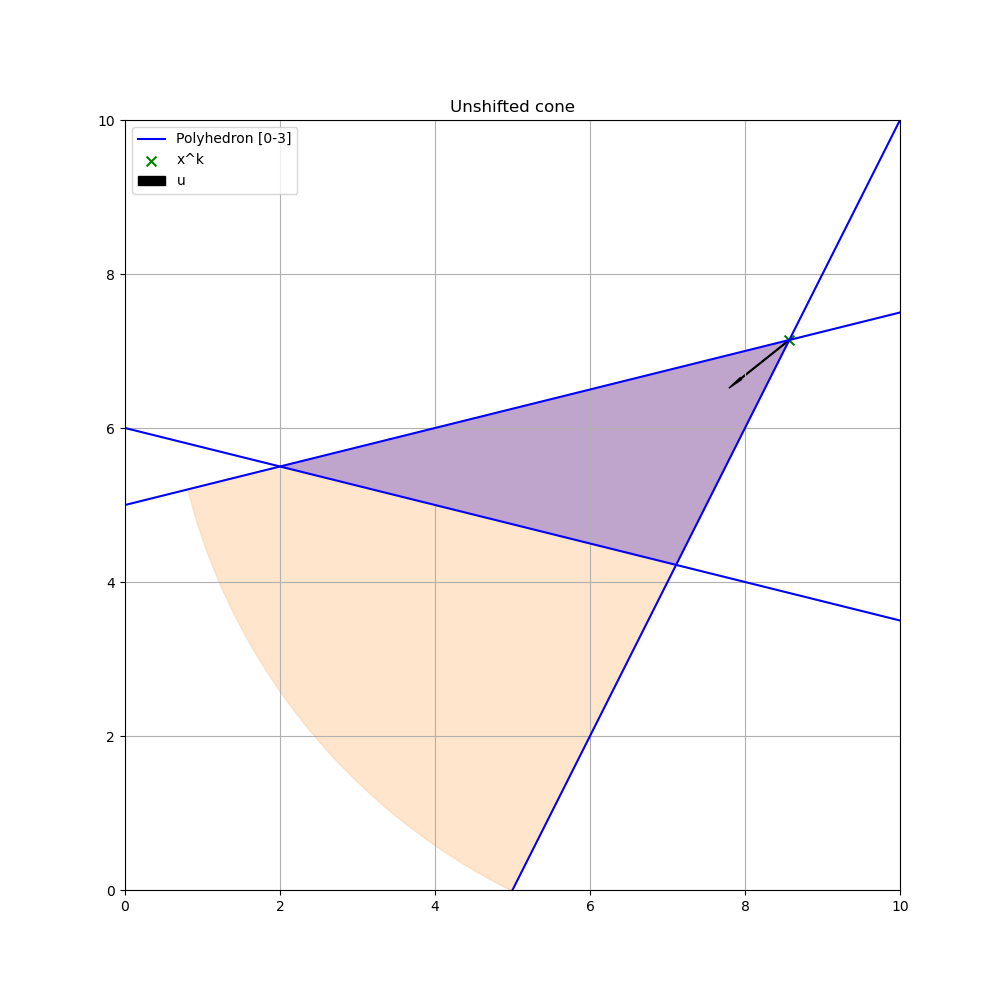
\includegraphics[width=200px]{images/unshifted_cone.png}
    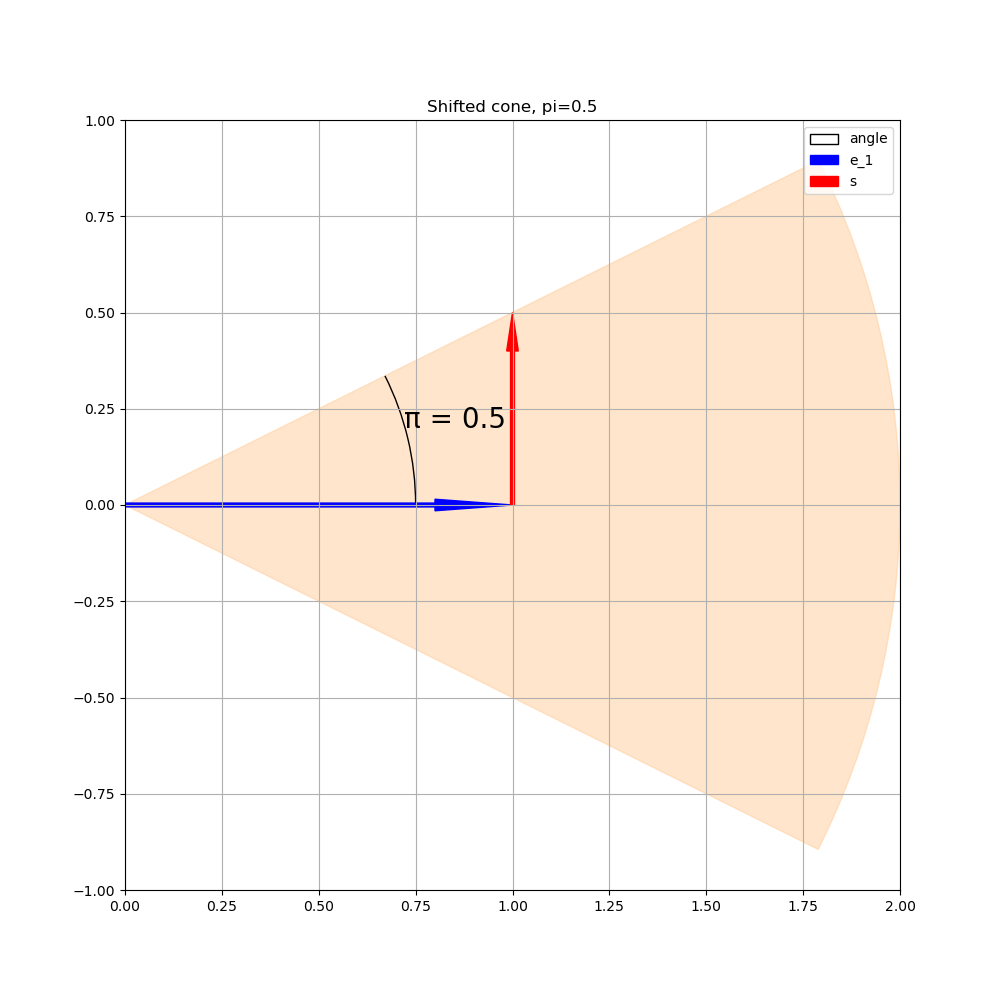
\includegraphics[width=200px]{images/shifted_cone.png}
    \caption[An example of the shifted and unshifted cones]
	{
		On the left is an unshifted cone $\unshiftedcone$.
		The zeros of the polyhedron constraint functions are in blue, and the current iterate is in green.
		A feasible direction $u$ from the current iterate is calculated, and the width of the cone is determined to lie within the active constraints of the polyhedra.
		On the right is a shifted cone $\unshiftedcone$.
		It is centered at the origin, and points along $e_1$, opening at a rate of $\alphak$.
    }
    \label{linear_cones_images}
\end{figure}

% \begin{boxedcomment}
% Illustrate the open rate...
% \end{boxedcomment}

Observe that, by construction, $\unshiftedcone$ is feasible with respect to the active constraints.
That is, $\lca_i x \le \lcb_i$ for all $x \in \unshiftedcone$ and $i \in \activei\left(\xk\right)$.
\cref{linear_cones_images} contains a depiction of these cones.


% = \left\{x \in \Rn \bigg | \quad x = \xk + t \uk+ s, s^Tu^{\star} = 0, t \ge 0, \|s\| \le {\alphak} t\right\}  \\
% \left\{x = (t, s)^T \in \Rn, t \in \mathbb R_{\ge 0}, s \in \mathbb R^{n-1} \bigg |\quad \|s\| \le {\alphak} t \right\} 

\begin{lemma}
\label[lemma]{unshiftedconeisfeasible}

Let $\unshiftedcone$ and $\polyk$ be defined by \cref{defineunshiftedcone} and \cref{polyhedron_k}.

The set $\unshiftedcone$ is feasible with respect to the active constraints of $\polyk$ at $\xk$.
\end{lemma}

\begin{proof}

Note that the trust region boundary cannot be active at $\xk$ as $\dk > 0$.
Let $\activei$, $\alphak$, and $\uk$ be defined by \cref{define_activei}, \cref{define_alpha_k}, \cref{define_u_k} and
$\lca$ and $\lcb$ be defined by \cref{eq:DFO-linear}.
Let $y = \xk + t\uk + s \in \unshiftedcone$ and $i \in \activei\left(\xk\right)$ be arbitrary.
Then,
\begin{align*}
{\lca}_{i}^Ty - {\lcb}_{i} = {\lca}_{i}^T(t\uk + s) = {\lca}_{i}^Ts + t {\lca}_{i}^T\uk \le \|s\| - \alphak t \le 0.
\end{align*}
\end{proof}

The following function is useful for showing results about our ellipsoids:
\begin{align}
f_{e}(\pi, \delta, r; x) = (x - \delta e_1)^T
\begin{pmatrix}
1 & \boldsymbol0^T \\
\boldsymbol 0 & \pi^{-2} \boldsymbol I \\
\end{pmatrix}
(x - \delta e_1) - r. \label{define_ellipsoid_function}
\end{align}

\begin{lemma}

\label[lemma]{shifted_ellipsoid_in_cone}
For any $\itbound \in (0, 2]$, let $\shiftedcone, f_e, \alphak$ be defined as in \cref{defineshiftedcone}, \cref{define_ellipsoid_function}, \cref{define_alpha_k}.
Then, for all $\delta > 0$, the ellipsoid
\begin{align}
\left\{x \in \Rn \bigg | f_e\left(\alphak, \delta, \frac {\delta^2}{\itbound^2}; x\right) \le 0 \right\} \subseteq \shiftedcone.
\end{align}
\end{lemma}

\begin{proof}

Suppose that $x \in \left\{x \in \Rn \bigg| f_e\left(\alphak, \delta, \frac {\delta^2}{\itbound^2}; x\right) \le 0 \right\}$,
and let $t = x^Te_1$, $s=x - t e_1$. 
Then $f_e(x) \le 0$ implies
\begin{align*}
\frac {\delta^2}{\itbound^2} \ge \frac {\delta^2}{2}&\ge
(x - \delta e_1)^T\begin{pmatrix}
1 & \boldsymbol0^T \\
\boldsymbol 0 & \left(\alphak\right)^{-2} \boldsymbol I \\
\end{pmatrix}(x - \delta e_1)  \\
& = (t - \delta)^2 + \frac {1} {\left(\alphak\right)^2} \|s\|^2 \\
\Longrightarrow \|s\|^2 &\le \left(\alphak\right)^2 \left[\frac {\delta^2}{2} - (t - \delta)^2\right] \\
&= \left(\alphak\right)^2 \left[t^2 - 2\left(t - \frac {\delta}{\itbound}\right)^2 \right] \le \left(\alphak\right)^2t^2 \\
\Longrightarrow \|s\| &\le \alphak t. \\
\end{align*}
Thus, $x \in\shiftedcone$.
\end{proof}

% \color{magenta}
% \begin{align*}
% \frac {\delta^2}{\itbound^2} - (t - \delta)^2 \le t^2 \\
% \frac {\delta^2}{\itbound^2} - t^2 + 2t\delta - \delta^2 \le t^2 \\
% \frac {\delta^2}{\itbound^2} + 2t\delta - \delta^2 \le 2t^2 \\
% \end{align*}
%
%
% \begin{align*}
% \frac {\delta^2}{\itbound^2} \ge \frac {\delta^2}2
% \end{align*}
%
% \color{black}






% \begin{align*}
% \delta^2 - (t - \delta)^2 \le t^2 \\
% \delta^2 - t^2 + 2 t\delta - \delta^2 \le t^2 \\
% 2 t\delta \le 2t^2 \\
% \delta \le t
% \end{align*}
% t^2 - 2\left(t^2 - t\delta + \frac 1 4 \delta^2 \right)
% = t^2 - 2 t^2 + 2 t\delta - \frac 1 2 \delta^2
% = - t^2 + 2 t\delta - \frac 1 2 \delta^2


\begin{lemma}
\label[lemma]{linear_mapping_works}

Let $\rotk$, $T_k$, $\unshiftedcone$, $\shiftedcone$ be defined as in
\cref{define_r}, \cref{define_affine_mapping}, \cref{defineunshiftedcone}, \cref{defineshiftedcone}.
Then $T_k\left(\unshiftedcone\right) = \shiftedcone$.
% and $T_k^{-1}(\shiftedcone) = \unshiftedcone$
\end{lemma}

\begin{proof}

Observe that $\rotk e_1 = \uk$, $\rotk \uk = e_1$, $\det(\rotk) = 1$, and 
$\rotk \rotk ^T = \rotk ^T\rotk = I$.

Suppose that $x \in \unshiftedcone$.
Then there exists $t \ge 0$ and $s \in \Rn$ such that $x = \xk + t \uk+ s$ where $s^T \uk = 0$ and $\|s\| \le {\alphak} t$.
Then $T_k(x) = t\rotk\uk + \rotk s = te_1 + \rotk s$.
Observe that $(Rs)_1 = (\rotk s)^Te_1 = s^T\rotk^T(\rotk \uk) = s^T \uk = 0$.
Hence,
$T_k(x) = \begin{pmatrix}
t \\
\sigma
\end{pmatrix}$ where $\sigma \in \mathbb R ^ {n-1}$ satisfies $\|\sigma\| = \|s\| \le \alphak t$.
Thus, $T_k(x) \in \shiftedcone$.
Conversely, if $\begin{pmatrix}
t \\
\sigma
\end{pmatrix} \in \shiftedcone$, then let
$s = \rotk^T\begin{pmatrix}
0 \\
\sigma
\end{pmatrix}$
to see that
$x = T_k^{-1}\left(\begin{pmatrix}
t \\
\sigma
\end{pmatrix} \right)= \rotk^T\left(t e_1 + \begin{pmatrix}
0 \\
\sigma
\end{pmatrix}\right) = t \uk + s$, where
$\|s\| = \|\sigma\| \le \alphak t$.
Hence $T_k^{-1}\left(\begin{pmatrix}
t \\
\sigma
\end{pmatrix}\right) \in \unshiftedcone$.
\end{proof}


\begin{lemma}
\label[lemma]{ellipsoid_fits}

Let $\activei$, $f_e$, $\deltaf$ $\alphak$, $\rotk$, $T_k$, and $\polyk$ be defined by
\cref{define_activei}, \cref{define_ellipsoid_function}, \cref{define_deltaf}, \cref{define_alpha_k}, \cref{define_r}, \cref{defineshiftedcone}, and \cref{polyhedron_k},
respectively.

For each iteration $k$, if $\activei\left(\xk\right) \ne \emptyset$, the ellipsoid
\begin{align}
\ellipsek = \left\{x \in \Rn \bigg | f_e\left(\alphak, \deltaf, \frac {\deltaf^2} {\itbound^2}; T_k(x)\right) \le 0\right\} \label{definefeasibleellipsoid}
\end{align}
satisfies $\ellipsek \subseteq \polyk$.
\end{lemma}

\begin{proof}


% Let $L$ be the shortest distance from $\xk$ to any point on a non-active constraint.
% Define $\alphakp = \sqrt{\left(1 + \left(\alphak\right)^2 \right) \left(1 + \frac 1 {\sqrt{2}}\right)}$, and let $\deltaf = \frac 1 {\alpha'} L$.

Let $\alphakp$, $\rotk$, $\unshiftedcone$, $\dnearcons\left(\xk\right)$, and $\shiftedcone$ be defined by
\cref{define_alphakp}, \cref{define_r}, \cref{defineunshiftedcone}, \cref{nearestnonactive}, and \cref{defineshiftedcone},
respectively.
We see that if $x \in \ellipsek$,
then by \cref{shifted_ellipsoid_in_cone} we have that $T_k(x) = \begin{pmatrix}t\\ \sigma\end{pmatrix} \in \shiftedcone$ for some $\sigma \in \mathbb R^{n-1}$
with $\left\|\sigma\right\| \le \alphak$, and
\begin{align*}
\frac {\deltaf^2}{\itbound} \ge
(x - \deltaf e_1)^T\begin{pmatrix}
1 & \boldsymbol0^T \\
\boldsymbol 0 & \left(\alphak\right)^{-2} \boldsymbol I \\
\end{pmatrix}(x - \deltaf e_1)
 = \left(t - \deltaf\right)^2 + \frac {1} {\left(\alphak\right)^2}\left\|\sigma\right\|^2
\ge (t - \deltaf)^2  \\
\Longrightarrow t \le \left(1 + \itbound^{-1}\right)\deltaf
\end{align*}
\color{magenta}
\begin{align*}
\frac {\deltaf^2} {\itbound^2} \ge (t - \deltaf)^2
\Longleftrightarrow \deltaf \ge \itbound (t - \deltaf)
\Longleftrightarrow \frac 1 {\itbound} \deltaf \ge  t - \deltaf
\Longleftrightarrow \left(1 + \itbound^{-1}\right) \deltaf \ge  t
\end{align*}
\color{black}
so that 
\begin{align*}
\|x\|^2 = t^2 + \|\sigma\|^2 \le t^2 + \left(\alphak\right)^2 t^2
\le \left[1 + \left(\alphak\right)^2 \right] \left(1 + \itbound^{-1}\right)^2\deltaf^2
= \left(\alphakp\right)^2 \deltaf^2 \\
\Longrightarrow \|x\| \le \alphakp \deltaf \le \dnearcons\left(\xk\right).
\end{align*}
Thus, all points within $\ellipsek$ are closer than the nearest point of a non-active constraint.
Combine this with \cref{unshiftedconeisfeasible} to see that $\ellipsek \subseteq \polyk$.
\end{proof}



\begin{lemma}
\label[lemma]{ellipsoid_includes_origin}

For any constant $\itbound > 1$, and any iteration $k$,
let $f_e$, $\deltaf$, $\rotk$, $T_k$, $\unshiftedcone$, $\shiftedcone$, $\polyk$ be defined as in
\cref{define_ellipsoid_function}, \cref{define_deltaf}, \cref{define_r}, \cref{define_affine_mapping}, \cref{defineunshiftedcone}, \cref{defineshiftedcone}, \cref{polyhedron_k}.

Then the ellipsoid
\begin{align}
\scaledellipsek  = \left\{x \in \Rn \bigg | f_e\left({\alphak}, \deltaf, \deltaf^2; T_k(x)\right) \le 0\right\} \label{definescaledfeasibleellipsoid}
\end{align}
satisfies $\xk \in \scaledellipsek$.
\end{lemma}

\begin{proof}

We have that
\begin{align*}
f_e\left(\alphak, \deltaf, \deltaf^2; T_k\left(\xk\right) \right)
&=
f_e\left({\alphak}, \deltaf, \deltaf^2; 0\right) \\
&=
(0 - \deltaf e_1)^T\begin{pmatrix}
1 & \boldsymbol0^T \\
\boldsymbol 0 & \left(\alphak\right)^{-2} \boldsymbol I \\
\end{pmatrix}(0 - \deltaf e_1) - \deltaf^2 \\
&= \deltaf^2 - \deltaf^2 = 0.
\end{align*}
\end{proof}








% 
% 
% 
% 
% We will first define the ellipsoid and show some of its properties within the transformed space $C_2$ before mapping it to $C_1$.
% To this end, fix an arbitrary $\delta > 0$ and let 
% $f_{e}(x): \Rn \to \reals $ be defined by 
% \begin{align}
% f_{e}(x) = (x - \delta e_1)^T\begin{pmatrix}
% 1 & \boldsymbol0^T \\
% \boldsymbol 0 & \alpha^{-2} \boldsymbol I \\
% \end{pmatrix}(x - \delta e_1) - \frac 1 2 \delta^2
% \label{define_ellipsoid_function}
% \end{align} 
% and consider the ellipsoid $E_1 = \{x | f_{e}(x) \le 0\}$.
% We will show that $E_1 \subseteq C_2$.
% To this end, suppose $x = (t, s) \in E_1$.
% Firstly, note that
% \begin{align*}
% 2\big(t - \frac {\delta} 2\big)^2 \ge 0
% \Longrightarrow 2t\delta - \frac 1 2 \delta^2 \le 2t^2 
% \Longrightarrow \frac 1 2 \delta^2 - (t - \delta)^2 \le t^2. 
% \end{align*}
% \Longrightarrow \frac 1 2 \delta^2 -t^2  + 2t\delta - \delta^2 \le t^2 \\
% \Longrightarrow 0 \le t^2 - t\delta + \frac 1 4 \delta^2
%  \Longrightarrow 0 \le 2t^2 - 2t\delta + \frac 1 2 \delta^2\\

% We choose this mapping because if $x = x_0 + t u^{\star} + s \in C_1$,
% then $\|s\|\le \alpha t \Leftrightarrow \|Rs\| \le \alpha t$ and $0 = s^Tu^{\star} = s^T R^T R u^{\star} = (Rs)^T e_1$ imply that 
% $R(x - x_0 - \delta u^{\star}) = t Ru^{\star} + Rs = t e_1 + Rs \in C_2$.
% Thus, the affine mapping $T : \Rn \to \Rn$ defined by $T(x) = R(x - x_0 - \delta u^{\star})$ maps $C_1$ to $C_2$.
% Conversely, the same arguments show that $T^{-1}(x) = R^Tx + x_0 + \delta u^{\star}$ maps $C_2$ to $C_1$.

%  \in SO(n)
% u = [3957; 6294.9]
% u = u / norm(u)
% e = [1; 0.0]
% a = e + u
% r = 2 * a * a' / (a' * a) - eye(2)
% r * e
% r * u


% 
% Having proven that $E_1 \subseteq C_2$, it follows that $T^{-1}(E_1) \subseteq C_2$.
% However, $T^{-1}(E_1) = \{ x \in \Rn | (x - \delta u^{\star})^TQ(x-\delta u^{\star} \le \frac 1 2 \epsilon\}$ where

% 
% \begin{align*}
% E_2 = \bigg \{x \bigg | (x - x_0 - \delta u^{\star})^T\bigg(R^T\begin{pmatrix}
% 1 & \boldsymbol0^T \\
% \boldsymbol 0 & \alpha^{-2} \boldsymbol I \\
% \end{pmatrix}R\bigg)(x - x_0 - \delta u^{\star}) \le \frac 1 2 \delta^2 \bigg\}.
% \end{align*}
% We know that $x \in E_1 \Leftrightarrow T(x) = R(x - x_0 - \delta u^{\star}) \in E_2 \Longrightarrow T(x) \in C_2 \Longrightarrow x = T^{-1}\left(T(x)\right) \in C_1$.
% Thus, we know that the ellipsoid $E_2$ is contained within the active constraints, and can be scaled by $2$ to include $x_0$.

\begin{lemma}
\label[lemma]{nontrivial_ellipsoid_exists}

Let $\activei$ and ${\alphak}$ be defined by \cref{define_activei} and \cref{define_alpha_k}, respectively.

Suppose that \cref{interior_point} holds.

For some iteration $k$, if $\activei \ne \emptyset$, then the ellipsoid defined by \cref{define_linear_nontrival_ellipsoid}
is suitable according to \cref{define_suitable_ellipsoid}.

% For iteration $k$, if ${\alphak} > 0$, then there exists a suitable ellipsoid for iteration $k$ according to .
\end{lemma}

\begin{proof}

\color{magenta}
For $\delta \in \left\{1, \itbound^2\right\}$:
\begin{align*}
\left(x - \ck\right)^T\qk\left(x - \ck\right) \le \delta \\
\Longleftrightarrow
\left(x - \xk+\deltaf \uk \right)^T\frac {\itbound^2} {\delta_f^2} \rotk^T \begin{pmatrix}
1 & \boldsymbol0^T \\
\boldsymbol 0 & \left({\alphak}\right)^{-2} \boldsymbol I \\
\end{pmatrix} \rotk\left(x - \xk+\deltaf \uk \right) \le \delta \\
\Longleftrightarrow
\left[\rotk\left(x - \xk\right)+\deltaf \rotk \uk \right]^T \begin{pmatrix}
1 & \boldsymbol0^T \\
\boldsymbol 0 & \left({\alphak}\right)^{-2} \boldsymbol I \\
\end{pmatrix} \left[\rotk\left(x - \xk\right)+\deltaf \rotk \uk \right] \le \frac 1 {\itbound^2} \delta\delta_f^2 \\
\Longleftrightarrow
\left(T_k(x) + \deltaf e_1 \right)^T \begin{pmatrix}
1 & \boldsymbol0^T \\
\boldsymbol 0 & \left({\alphak}\right)^{-2} \boldsymbol I \\
\end{pmatrix} \left(T_k(x) + \deltaf e_1 \right) - \frac 1 {\itbound^2} \delta\delta_f^2 \le 0\\
\left[
\Longleftrightarrow (x - \delta e_1)^T
\begin{pmatrix}
1 & \boldsymbol0^T \\
\boldsymbol 0 & \pi^{-2} \boldsymbol I \\
\end{pmatrix}
(x - \delta e_1) - r \le 0 \right]\\
\Longleftrightarrow f_{e}(\alphak, \deltaf,\frac 1 {\itbound^2} \delta\delta_f^2; T_k(x)) \le 1
\end{align*}

\color{black}

Let 
$f_e$,
$T_k$,
$\rotk$, $\deltaf$, and $\scaledunshiftedellipsoid$
be defined as in
\cref{define_ellipsoid_function},
\cref{define_affine_mapping},
\cref{define_r},
\cref{definefeasibleellipsoid}, and
\cref{definescaledfeasibleellipsoid},
respectively. 
Observe that \cref{define_suitable_ellipsoid} with \cref{define_linear_nontrival_ellipsoid} defines  $\ellipsek$ and $\scaledellipsek$ to be
\begin{align*}
\begin{array}{cccc}
\ellipsek &=& \left\{x \in \Rn \bigg | f_e\left(\alphak, \deltaf, \frac {\deltaf^2} {\itbound^2} ; T_k(x)\right) \le 0\right\}, &\quad \textrm{and}  \\
\scaledellipsek &=& \left\{x \in \Rn \bigg | f_e\left({\alphak}, \deltaf, \deltaf^2; T_k(x)\right) \le 0\right\}.&
\end{array}
\end{align*}

By \cref{ellipsoid_fits}, we know that $\ellipsek \subseteq \polyk$.
By \cref{ellipsoid_includes_origin}, we know that $\xk \in \scaledellipsek$ .
By \cref{alphas_are_bounded}, there exists $\epsilon_{\alpha} > 0$, such that the condition number 
$\condition\left(\qk\right) = \frac{\max\{1, {\alphak}^{-2}\}}{\min\{1, {\alphak}^{-2}\}} = \left({\alphak}\right)^{-2} > 0$.
This is because $\det\left(\rotk\right) = 1$ means the condition number of $\qk$ is not affected $\rotk$.
\end{proof}


\section{Results}

% Here, we present numerical results for our implementations of \cref{linearly_constrained_dfo_simple}.

\subsection{Hock-Schittkowksi test problems}


We tested these algorithms on several problems from the Hock-Schittkowski problem set \cite{Schittkowski1981MoreTE} and \cite{Hock1980}.
We selected the problems that have linear constraints: 21, 24, 25, 35, 36, 44, 45, 76, 224, 231, 232, 250, 251.
We summarize the results within \color{magenta} a section to come \color{black}.

% 37 was left out because it proved to be difficult.

\paragraph*{Performance profile.}
\label{performance_profile}
In order to better evaluate the algorithms on the problems across in this test set, we use a performance profile developed in \cite{More:2009:BDO:1654367.1654371}.
Given a set of Solvers $\mathcal S$ that solved a set of problems $\mathcal P$ with the number of evaluations of solver $s$ on problem $p$ being $N(s, p)$, the performance ratio is defined to be $r(s, p) = \frac{N(s, p)}{\min_{s \in \mathcal S} N(s, p)}$.
If the algorithm does not complete, then the number of evaluations is set to $\infty$.
The performance profile of a solver $s$ and parameter $\alpha \in [0, \infty)$ is then the number of problems for which the performance ratio is less than or equal to $\alpha$: 

\begin{align}
\rho(s, \alpha) = \frac 1 {\left\|\mathcal P \right\|} \left\|p \in \mathcal P | r(s, p) \le \alpha\right\|.
\end{align}

The $y$ axis of a performance plot is the performance profile, and the $x$ axis is the parameter $\alpha$.
Note that algorithms with high performance profiles for small values of $\alpha$ solved a large number of problems the most with the fewest evaluations, while algorithms that eventually reach high performance profiles with larger values of $\alpha$ solve a large set of problems.
The performance profile for the Hock-Schittkowski problem set is given in figure \cref{performance_profile_image}.

	
\begin{figure}[ht]
    \centering
    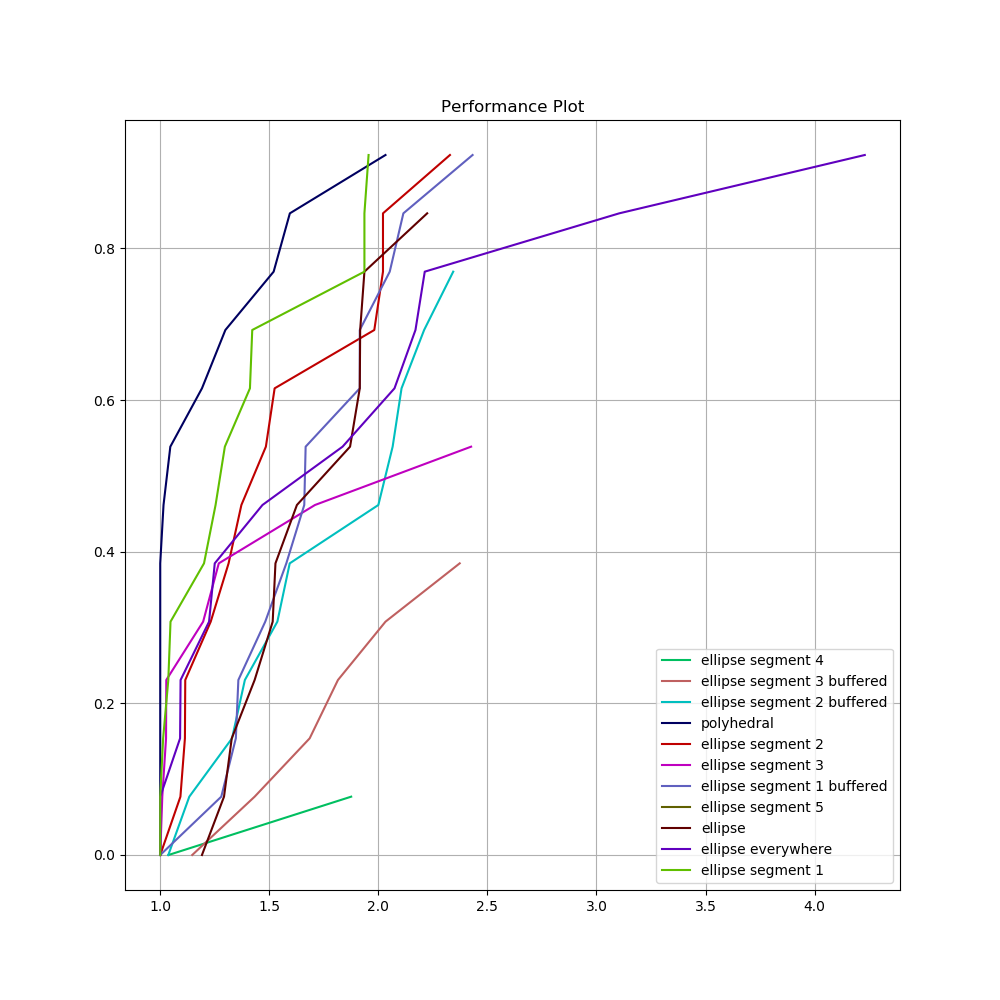
\includegraphics[scale=0.4]{images/performance_profile_plot.png}
    \caption[A performance profile comparing variants of the algorithm for linear constraints.]{
    	A performance profile comparing different variants of the algorithm for linear constraints.
    	We see that the polyhedral algorithm is both efficient and robust.
    }
    \label{performance_profile_image}
\end{figure}



% The line segment search with 5 segments does not solve many problems, this is because several of the problems have dimension less than $5$, so that it was not even run on these.
% Notice that the polyhedral search does very well.
% We conjecture that this may not hold with modeled, nonlinear constraints.



% \color{red}
% 
% \section{Figure out where goes}
% 
% From here on, we will assume that the iterates $\xk$ are chosen according to \cref{linearly_constrained_dfo}.
% This implies that each of the sample points used to construct $\mfk$ are output of \cref{model_improving_algorithm}.
% 
% Because \cref{lipschitz_gradient} and \cref{lipschitz_hessian} are satisfied, $f$ also satisfies \cref{introduction_3_1} and hence the assumptions for \cref{quadratic_errors}.
% Notice that because $\kappa_f$, $\kappa_g$, $\kappa_h$ only depend on $p$, $L_h$, and $\Lambda$, these values do not depend on the iteration $k$:
% using the same tolerance $\xi_{\text{min}}$ within \cref{model_improving_algorithm} implies a bound on $\Lambda$.
% , and therefore $\mfk$ satisfies the requirements for \cref{quadratic_errors}.
% is a fully quadratic model over $B_{\infty}(\xk, \dk)$.
% \color{black}


\bibliography{thesis}
\bibliographystyle{ieeetr}
\end{document}
